%\documentclass{report}
\documentclass{scrartcl}
\setlength{\parindent}{0in}
\makeatletter
\DeclareOldFontCommand{\rm}{\normalfont\rmfamily}{\mathrm}
\DeclareOldFontCommand{\sf}{\normalfont\sffamily}{\mathsf}
\DeclareOldFontCommand{\tt}{\normalfont\ttfamily}{\mathtt}
\DeclareOldFontCommand{\bf}{\normalfont\bfseries}{\mathbf}
\DeclareOldFontCommand{\it}{\normalfont\itshape}{\mathit}
\DeclareOldFontCommand{\sl}{\normalfont\slshape}{\@nomath\sl}
\DeclareOldFontCommand{\sc}{\normalfont\scshape}{\@nomath\sc}
\makeatother

\usepackage{multirow}

\usepackage[utf8]{inputenc}
\usepackage{amsmath}
\numberwithin{equation}{section}
\usepackage{amssymb}
\usepackage{lscape}

\usepackage{algorithmic}
\usepackage{algorithm}
\renewcommand{\algorithmicrequire}{\textbf{Input:}}
\renewcommand{\algorithmicensure}{\textbf{Output:}}

\usepackage[dvipsnames]{xcolor}
\usepackage{yfonts}
\usepackage[T1]{fontenc}
\usepackage[toc,page]{appendix}


\usepackage{graphicx}
\usepackage{subcaption}
\usepackage[hidelinks]{hyperref}
\usepackage{blkarray}
\usepackage{cancel}
\usepackage{enumitem}
\usepackage{listings}
\usepackage{color}
\usepackage{pdfpages}
\usepackage{helvet}
\usepackage{tikz}
\usetikzlibrary{graphs}


\definecolor{dkgreen}{rgb}{0,0.6,0}
\definecolor{gray}{rgb}{0.5,0.5,0.5}
\definecolor{mauve}{rgb}{0.58,0,0.82}
\definecolor{babyblueeyes}{rgb}{0.63, 0.79, 0.95}

\lstdefinestyle{base}{
  inputencoding=latin10,
  emptylines=1,
  breaklines=true,
  basicstyle=\small\ttfamily,
  moredelim=**[is][\color{red}]{@}{@},
}

\newcommand{\norm}[1]{\left\lVert#1\right\rVert}

%% Define a HUGE 
\makeatletter
\newcommand\HUGE{\@setfontsize\Huge{24.88}{50}}
\makeatother

\begin{document}             % End of preamble and beginning of text.

 
%titlepage
\thispagestyle{empty}
\begin{center}
\begin{minipage}{.9\linewidth}
\flushright
	      		 
	%University logo
    
\includegraphics[width=0.5\linewidth]{univie.eps}\par
\centering 	
    % Title
	{\scshape{\HUGE Bachelorarbeit\par}}
	\vspace{1cm}
	%Thesis title
    {\scshape{\Large Implementation and experimental comparison between the COMMUNICATION AVOIDING-GENERALIZED MINIMAL RESIDUAL METHOD and standard GMRES \par}}
    \vspace{2cm}
    
  
 Verfasser  \linebreak
 {\Large Robert Ernstbrunner \par}
 	\vspace{.7cm}
angestrebter akademischer Grad\linebreak
 {\Large Bachelor of Science (BSc)\par}
	\vspace{.7cm}

\flushleft
	

\begin{tabular}{ll}
Wien, 2019	\linebreak
\vspace{.5cm}&   \\
  Studienkennzahl lt. Studienblatt: & A 033 521 \vspace{.3cm} \\ 
  Fachrichtung: & Informatik  - Scientific Computing
  \vspace{.3cm} \\
  Betreuerin / Betreuer: & Univ.-Prof. Dipl.-Ing. Dr.\\ 
  & Wilfried Gansterer, M.Sc. \\
 \end{tabular}
 

\end{minipage}
\end{center}
\clearpage

\pagebreak

\tableofcontents

\pagebreak

\section{Notation}
Similar notation is considered as in Hoemmen et al. \cite{Hoemmen:2010:CKS:1970638} and Grigori et al. \cite{Grigori}.
\subsection*{Linear Algebra}
\begin{itemize}
\item Greek letters denote scalars, lower case Roman letters denote vectors (or - based on the context - dimensions), capital Roman letters denote matrices.
\item Capital letters with two subscripts, e.g. '$V_{m, n}$', denote matrices with $m$ rows and $n$ columns.
\item Capital \textit{Black letter} letters (e.g. $V$, $Q$ and $R$ in Black letters are represented by $\mathfrak{V}$, $\mathfrak{Q}$ and $\mathfrak{R}$ resp.) denote matrices that are composed out of other matrices. 
\item $v_k$ denotes the $k^{th}$ vector in a series of vectors $v_0$, $v_1$, $\ldots$, ,  $v_k$, $v_{k+1}$, $\ldots$ of equal length.
\item Similarly, $V_k$ denotes the $k^{th}$ matrix in a sequence of matrices $V_0$, $V_1$, $\ldots$ , $V_k$, $V_{k+1}$, $\ldots$. Generally all these matrices have the same number of rows. They may or may not have the same number of columns.
\item If $V$ is a matrix consisting of $s$ vectors $\left[v_1, v_2, \ldots, v_s\right]$, then $\underline{V} = \left[V, v_{s+1} \right]$. The underline denotes one more column at the end.
\item If again, $V$ is a matrix consisting of $s$ vectors $\left[v_1, v_2, \ldots, v_s\right]$, then $\acute{V} = [v_2, v_3, \ldots, v_s]$. The acute denotes one column less at the beginning.
\item As a consequence $\underline{\acute{V}}$ denotes one more column at the end and one less column at the beginning, e.g. $\underline{\acute{V}} = [\acute{V}, v_{s+1}]$.
\item Depending on the context, both underline or/and acute letters can also refer to rows as well. 
\item $0_{m, n}$ is defined as an $m \times n$ matrix consisting of zeros, $I_{m}$ denotes the $m \times m$ Identity matrix and $e_k$ denotes the $k^{\text{th}}$ canonical vector with the dimension depending on the context.
\item All matrices and vectors are assumed to be real, if not stated otherwise.
\item Matlab notation is used for addressing elements of matrices and vectors. For example, given a matrix $A$ of size $n \times n$ and two sets of indices $\alpha$ and $\beta$, $A(\alpha,:)$ is a submatrix formed by the subset of the rows of $A$ whose indices belong to $\alpha$. Similarly, $A(\alpha, \beta)$ is a submatrix formed by the subset of the rows of $A$ whose indices belong to $\alpha$ and the subset of the columns of $A$ whose indices belong to $\beta$.
\end{itemize}
\subsection*{Terms and definitions}
\begin{itemize}
\item \textbf{Fetching}: the movement of data. This could either be \textit{reading} , \textit{copying} or \textit{sending} and \textit{receiving} messages.
\item \textbf{Ghosting}: the storage of redundant data that does not belong to a processors assigned domain.
\end{itemize}
\subsection*{Graph Notation}
\begin{itemize}
\item $G(A)$ denotes the directed graph of $A$ with $G(A) = \{V,E\}$ where $V(G(A))$ is the set of vertices of $G(A)$ and $E(G(A))$ is the set of edges of $G(A)$.
\item $R(G(A), \alpha)$ denotes the set of vertices in $G(A)$ that are reachable from any vertex in the set $\alpha$, including $\alpha$.
\item $R(G(A), \alpha, m)$ denotes the set of vertices in $G(A)$ that are reachable by paths of length at most $m$ from any vertex in $\alpha$, including $\alpha$.
\end{itemize}
\subsection*{Abbreviations}
\begin{itemize}
\item \textbf{MPK}: Matrix powers kernel
\item \textbf{TSQR}: Tall and skinny QR factorization
\item \textbf{CGS}: Classical Gram-Schmidt method
\item \textbf{MGS}: Modified Gram-Schmidt method
\item \textbf{BCGS}: Block Classical Gram-Schmidt method
\item \textbf{MKL}: Intel Math Kernel Library
\end{itemize}
\pagebreak

\begin{abstract}
Abstract
\end{abstract}
\section{Introduction}
As the CPU-memory performance gap widens the cost for communication increases as well.

Compared to arithmetic costs communication costs are much higher and the widening CPU-memory performance gap promotes the need for communication-avoiding algorithms.\\

The CA-GMRES algorithm was implemented in a shared-memory environment.

Communication avoiding GMRES is based on s-step GMRES 
\cite{Erhel95aparallel}
\\

The term \textit{communication} generally denotes the movement of data either between different processors in the parallel case or between 'fast' and 'slow' memory in the sequential case, where 'fast' and 'slow' are relative to the two levels examined in the memory hierarchy (e.g., cache and DRAM, or DRAM and disk). Communication optimal algorithms do not eliminate communication completely, but they are constructed in a way such that reduction of communication is prioritized. This often results in new challenges, e.g., the  CA-ILU(0) algorithm (Section~\ref{sec:ca-ilu}) has to balance between communication and redundant computations; CA-GMRES (Section~\ref{sec:ca-gmres}) incorporates additional techniques to deal with ill-conditioned basis vectors.

\pagebreak
\section{Related work}
s-step methods, CA-ILU(0)
\pagebreak

\section{GMRES}
The Generalized Minimal Residual Method (GMRES) was first introduced by Saad et al. \cite{Saad:1986:GGM:14063.14074} and is an iterative Krylov subspace method for solving large sparse linear systems. 
The GMRES method starts with an initial approximate solution $x_0$ and initial residual $r_0 = b - Ax_0$ and finds a correction $z_k$ at iteration $k$ which solves the least-squares problem 
\begin{equation}
	z_k := \text{argmin}_{z} \norm{b - A(x_0 + z)}_2
\end{equation}
where $z_k$ is determined in the Krylov subspace 
\begin{equation*}
	 \mathcal{K}_k(A, r_0) = \text{span}\{r_0, Ar_0, \ldots, A^{k-1}r_0\}.
\end{equation*}
The solution at iteration $k$ is then formed by $x_k = x_0 + z_k$.
Since $\{r_0, Ar_0, \ldots, A^{k-1}r_0\}$ is usually ill-conditioned the Arnoldi method is incorporated to produce $k + 1$ orthonormal basis vectors $\underline{Q} = [q_1, q_2, \ldots, q_k, q_{k + 1}]$ with $q_1 = r_0/\norm{r_0}_2$ and a $k + 1 \times k$ upper Hessenberg coefficient matrix $\underline{H}$ where
\begin{equation*}
	AQ = \underline{Q}\underline{H}.
\end{equation*}
With these conditions $z_k$ can be defined as $z := Qy$ such that 
\begin{eqnarray*}
	\text{argmin}_{z} \norm{b - A(x_0 + z)}_2 &=& \text{argmin}_y \norm{r_0 - AQy}_2 \\
	 &=& \text{argmin}_{y} \lVert r_0 - \underline{Q} \underline{H} y \rVert_2.
\end{eqnarray*}
Since $q_1 = r_0/\norm{r_0}_2$ and $\underline{Q}$ is orthonormal, one has
\begin{eqnarray} \label{eq:stdgmreslsp}
	\text{argmin}_y \lVert r_0 - \underline{Q} \underline{H} y \rVert_2 &=& \text{argmin}_{y} \lVert \underline{Q}^T r_0 - \underline{H} y \rVert_2 \nonumber \\
	&=& \text{argmin}_{y} \norm{\beta e_1 - \underline{H} y}_2 
\end{eqnarray}
with $\beta = \norm{r_0}_2$.
$\underline{H}$ is then factored into $\underline{H} = \underline{G}\underline{U}$ with square matrix $\underline{G}$ being a product of $k$ Givens rotations, $\underline{U} = 
\begin{pmatrix}
	U \\
	0_{1, k}
\end{pmatrix}$
and $U$ being upper triangular. Also, $g$ is defined by $\underline{g} := \beta \underline{G}^T e_1$ without the last entry. The triangular system to solve is then given by
\begin{equation*}
	y_k := \text{argmin}_y \norm{g - U y}_2
\end{equation*}
The solution at iteration $k$ is obtained by computing $x_k = x_0 + Qy_k$. Note that the absolute value of the last coordinate of $\underline{g}$ is $\norm{b - Ax_k}_2$, the absolute residual at iteration $k$.

\begin{algorithm}
\caption{GMRES(m)}
\label{alg:gmres(m)}
\begin{algorithmic}[1]
    \REQUIRE $n \times n$ linear system $Ax = b$ and initial guess $x_0$
    \STATE restart := true
    \WHILE{restart}
    	\STATE $r_0:=b - Ax_0$, $\beta := \norm{r_0}_2$, $q_0 := r_0/\beta$, $\underline{Q}_0 := q_0$, $\underline{H}_0 := \varnothing$
    	\FOR{$k = 1$ to $m$}
			\STATE Compute $q_k$ and $h_k$ using Algorithm~\ref{alg:mgs_arnoldi}
			\STATE Set $\underline{Q}_k := [Q_{k-1},q_k]$ and $\underline{H}_k := [\underline{H}_{k -1}, h_k]$
			\STATE Reduce ${h_k}$ of $\underline{H}_k$ from upper Hessenberg to upper triangular form using $k$ \\
		\hspace{\algorithmicindent} Givens rotations $G_1$, $G_2$, $ \ldots$, $G_{k}$. Apply the same rotations in the same order \\ 
		\hspace{\algorithmicindent} to $\beta e_1$,  resulting in the length $k + 1$ vector $\zeta_{k}$.
			\STATE Element $k + 1$ of $\zeta_k$ is the 2-norm (in exact arithmetic) of the current residual \\
\hspace{\algorithmicindent} $r_{k + 1} = b - Ax_{k + 1}$ of the current solution $x_{k + 1}$.
		\IF{converged}
			\STATE restart = false, and exit for loop		
		\ENDIF
		\ENDFOR
		\STATE Use the above reduction of $\underline{H}_k$ to upper triangular form and $\zeta_k$ to solve $y_k :=$ \\ \hspace{\algorithmicindent} $\text{argmin}_{y} \norm{\underline{H}_k y - \beta e_1}_2$
		\STATE Set $x_0 := x_0 + Q_k y_k$
	\ENDWHILE 
\end{algorithmic}
\end{algorithm}

\section{Computational kernels}
%introduction; definitions: kernel, communication-avoiding
In this thesis \textit{computational kernels} define parts of an algorithm with significantly high costs, relatively speaking. These costs include both arithmetic operations and communication. The following kernels make up the essential building blocks in Arnoldi($s,t$) (see Section~\ref{sec:ca_arnoldi}) and eventually CA-GMRES (see Section~\ref{sec:ca-gmres}).


\subsection{Matrix powers kernel}
The matrix powers kernel, as described by Hoemmen et al. in \cite{Hoemmen:2010:CKS:1970638}, was not implemented in the context of this thesis. However, it is an essential part to avoid communication and therefore, will be briefly summarized here.\\
In its basic form, the MPK takes an $n \times n$ matrix $A$ and a starting vector $v_1$ as input and produces $s$ more vectors $Av, A^2v, \ldots, A^sv$. Since $A$ is usually large and sparse, it makes sense to also look at the graph of $A$, namely $G(A)$ in order to apply known graph algorithms. In $s$-step methods, the MPK replaces the sparse matrix-vector products that generate the basis for the Krylov subspace $\mathcal{K}_{s + 1}(A, v) = \left[v, Av, A^2v, \ldots, A^{s}v\right] = \left[v_1, v_2, \ldots, v_{s + 1}\right]$. One invocation of the MPK produces the same amount of basis vectors as $s$ sparse matrix-vector products. The MPK sends a factor of $\Theta(s)$ fewer messages than $s$ SpMV invocations and the matrix has to be read from slow to fast memory only once.
In order to achieve this, the data and the workload are distributed among $P$ processors, where each processor is assigned a part $\alpha$ of $A(\alpha,:)$ and $v_1(\alpha)$ with $\alpha \subseteq V(G(A))$. Then, each processor fetches $A(\eta,:)$ and $v_1(\eta)$, with $\eta = R(G(A), \alpha, s) - \alpha$ in order to compute $s$ more vectors $v_2(\alpha), v_3(\alpha), \ldots, v_{s + 1}(\alpha)$ without communication. In other words, to compute $v_2(\alpha)$, the superset $\beta = R(G(A),\alpha, 1)$ is required. To compute $v_3(\alpha)$, the set $R(G(A),\beta, 1) = R(G(A),\alpha, 2)$ must be available. In general, to compute $v_{s + 1}(\alpha)$, the set $R(G(A),\alpha, s)$ must be at hand. Since
\begin{equation*}
\alpha \subseteq R(G(A),\alpha, 1) \subseteq \ldots \subseteq R(G(A),\alpha, s - 1) \subseteq R(G(A),\alpha, s)
\end{equation*} it is clear, that larger steps eventually lead to increasing amounts of ghosted data and floating point operations.

\subsubsection{Preconditioned matrix powers kernel}
Iterative Krylov methods often require a preconditioner that, when applied, fundamentally changes the MPK. In order to avoid communication, highly parallelizable preconditioners come to mind. E.g., Nuentsa et al. \cite{nuen11c} present their parallel GMRES with a multiplicative Schwarz preconditioner. Grigori et al. \cite{Grigori} developed \textit{CA-ILU(0)}, a very interesting type of preconditioner that, at first glance, seems unfit for a parallel and communication-avoiding environment. Section~\ref{sec:ca-ilu} summarizes their work.

\iffalse
\cite{Hoemmen:2010:CKS:1970638} p.60\\
The Matrix Powers Kernel 
Power iteration, SpMV instead of MV, sparse matrix like a graph $\rightarrow$ spacial, temporal locality not as efficiently used as in dense MV. 
Avoid communication by sending / receiving all necessary values beforehand (look at reachability of graph(A)) and computing s basis vectors without further communication.\\
\texttt{To minimize communication in a parallel setting, the s Monomial basis vectors of the Krylov subspace $[y, Ay, A2y, \ldots, A^sy]$ are computed with no communication using the so-called matrix powers kernel [13]. This requires ghosting and computing redundantly on each processor the data required for computing its part of the vectors with no communication. Note that throughout this paper we use the term ghosting to denote the storage of redundant data, of vectors or matrices, that do not belong to the processor's assigned domain or part, but are needed for future computations.\\
First, the data and the work is split between $P$ processors. Each processor is assigned a part $\alpha$ of the input vector $y_0$ ($y_0(\alpha)$) and $A(\alpha, :)$, where $\alpha \subseteq V(G(A))$. Then, each processor has to compute the same part $\alpha$ of $y_1 = Ay_0$, $y_2 = Ay_1$, till $y_s = Ay_{s - 1}$ without communicating with other processors. To do so, each 
processor fetches all the data needed from the neighboring processors, to compute its part $\alpha$ of the $s$ vectors. Thus, to compute $y_s(\alpha)$, each processor should receive the missing data of $y_0(\eta_s)$ and $A(\eta_s, :)$ from its neighboring processors and store it redundantly, where $\eta_s = R(G(A), \alpha, s)$. Finally, each processor computes the set $R(G(A), \alpha, s - i)$ of the vectors $y_i$ for $i = 1, 2, \ldots, s$ without any communication with the other processors.}
\fi

\subsection{Tall and skinny QR}
TSQR is a QR decomposition algorithm especially suited for $m \times n$ matrices, where $m \gg n$. TSQR uses a divide-and-conquer approach and therefore, works on a reduction tree structure. The highest form of parallelism is achieved if TSQR uses a binary tree. In the purely sequential case a linear (flat) tree comes into play. Hybrid algorithms use anything in between and the best tree structure may depend on the matrix size and underlying architecture as Demmel et al. explain in~\cite{Demmel:2012:CA-QR_demmel}. The parallel TSQR with a binary tree is summarized below. For a more detailed description, as well as a description of the sequential algorithm, see Demmel et al.~\cite{Demmel:2012:CA-QR_demmel}.
\paragraph{Parallel TSQR} First, the matrix $A$ is split up into $P$ parts with each submatrix having size $m/P \times n$. TSQR on a binary tree then passes $P - 1$ stages where any fast and accurate QR factorization can be applied for each stage. Let's assume $P = 4$, then 
\begin{equation*}
A =
\begin{pmatrix}
A_0\\A_1\\A_2\\A_3
\end{pmatrix}.
\end{equation*}
At stage zero the QR factorization for each submatrix $A_i$ is computed, with
\begin{equation*}
A_0 = Q_{00}R_{00}, \qquad A_1 = Q_{10}R_{10}, \qquad A_2 = Q_{20}R_{20} \quad \text{and} \quad A_3 = Q_{30}R_{30}.
\end{equation*}
The successive stage merges the $R$-factors and computes the next QR-factorizations
\begin{equation*}
\begin{pmatrix}
R_{00} \\
R_{10}
\end{pmatrix} =
Q_{01}R_{01} \qquad \text{and} \qquad
\begin{pmatrix}
R_{20} \\
R_{30}
\end{pmatrix} = 
Q_{11}R_{11}.
\end{equation*}
This procedure is repeated until one last QR factorization is performed where the final $R$ factor can be interpreted as the root of the tree. This results in the following decomposition
\begin{equation} \label{eq:tsqr}
A =
\begin{pmatrix}
A_0\\A_1\\A_2\\A_3
\end{pmatrix} =
\left(
	\begin{array}{c|c|c|c}
	Q_{00} & & & \\
	\hline
	& Q_{10} & & \\
	\hline
	& & Q_{20} & \\
	\hline
	& & & Q_{30}
	\end{array}
	\right) \cdot
\left(
	\begin{array}{c|c}
		Q_{01} & \\
		\hline
		& Q_{11} 
	\end{array}
\right) \cdot
Q_{02} \cdot R_{02}.
\end{equation}

Figure~\ref{fig:tsqr} shows, that this approach only requires $\mathcal{O}(\log P)$ messages on $P$ processors (a factor of $\Theta (s)$ fewer messages than Householder QR or MGS). \cite{Demmel:2012:CA-QR_demmel} show that, sequentially, the matrix is read only once, saving a factor of $\Theta(s)$ transferred data between levels of the memory hierarchy (compared to Householder QR or MGS). 
Of course,~\eqref{eq:tsqr} is stored implicitly to save storage space.\\
The orthogonality of the $Q$ factor computed by Classical or Modified Gram-Schmidt depends on the condition number of $A$. Householder QR, on the other hand, does not make any assumptions on $\mathcal{K}(A)$, it is \textit{unconditionally} stable. Therefore, Householder QR is a good choice for the local QR factorizations in TSQR, which makes TSQR inherently unconditionally stable as well.\\

For reasons explained in Section~\ref{sec:scaling_first_basis_vec} one might want TSQR to produce an $R$ factor with real nonnegative diagonal entries. Demmel et al. show in $\cite{doi:10.1137/nonnegdiags_demmel} $ how to modify the usual Householder QR in a numerically stable way so that such a factor is generated. This modified Householder QR factorization can then be incorporated, in order to let TSQR as well produce an $R$ factor with real nonnegative diagonal entries.


\begin{figure}
	\centering
\tikz [new set = A,
	   new set = Q,
	   new set = QQ,
	   new set = R,
	   new set = RR
	   ] {

\node [set = A, rectangle, minimum width=0.7cm, fill=babyblueeyes] at (1,3) {$A_0$};
\node [set = A, rectangle, minimum width=0.7cm, fill=babyblueeyes] at (1,2) {$A_1$};
\node [set = A, rectangle, minimum width=0.7cm, fill=babyblueeyes] at (1,1) {$A_2$};
\node [set = A, rectangle, minimum width=0.7cm, fill=babyblueeyes] at (1,0) {$A_3$};
\node (Q00) [set = Q] at (2.5,3) {$Q_{00}$};
\node (Q10) [set = Q] at (2.5,2) {$Q_{10}$};
\node (Q20) [set = Q] at (2.5,1) {$Q_{20}$};
\node (Q30) [set = Q] at (2.5,0) {$Q_{30}$};
\node [set = R, rectangle,
		minimum height=1.6cm,
		minimum width=0.7cm,
		align=center,
		fill=babyblueeyes] at (3.2,2.5) {};
\node [set = R, rectangle,
		minimum height=1.6cm,
		minimum width=0.7cm,
		align=center,
		fill=babyblueeyes] at (3.2,0.5) {};

\node (Q01) [set = QQ] at (4.7, 2.5) {$Q_{01}$};

\node (Q11) [set = QQ] at (4.7, 0.5) {$Q_{11}$};

\node [set = RR, rectangle,
		minimum height=2.6cm,
		minimum width=0.7cm,
		align=center,
		fill=babyblueeyes] at (5.4, 1.5) {};

\node (Q02R02) [set = QQ] at (7.2, 1.5) {$Q_{02}R_{02}$};

\node (R01) at (5.4, 2.5) {$R_{01}$};
\node (R11) at (5.4, 0.5) {$R_{11}$};
\node (R00) at (3.2, 3) {$R_{00}$};
\node (R10) at (3.2, 2) {$R_{10}$};
\node (R20) at (3.2, 1) {$R_{20}$};
\node (R30) at (3.2, 0) {$R_{30}$};

\graph { 
	(A) ->[matching] (Q),
	(R) ->[matching] (QQ),
	(RR) ->[matching] (Q02R02)
	};
}
\caption{Parallel TSQR on a binary tree of four processors. The first subscript of the $Q$ and $R$ matrices indicates the sequence number for a stage, the second subscript is the stage number. The blue boxes represent the processors involved at each stage.}
\label{fig:tsqr}
\end{figure}

\subsection{Block Gram-Schmidt} \label{sec:gs}
The Gram-Schmidt process takes a set of $s$ linearly independent basis vectors $V = [v_1, \ldots, v_s]$ and creates an orthonormal basis that spans the same subspace as $V$. Unlike unblocked Gram-Schmidt methods, blocked Gram-Schmidt algorithms work on blocks of columns at a time instead of one column at a time. If the matrix consists of $s$ columns this usually requires a factor of $\Theta (s)$ fewer messages and a factor of $\Theta(s)$ fewer data transfers between levels of the memory hierarchy.\\
In their performance analysis with a simplified parallel model, Hoemmen et al. \cite{Hoemmen:2010:CKS:1970638} also show that blocked classical Gram-Schmidt is superior to a blocked modified Gram-Schmidt variant in terms of the messages sent between processors. However, they state that BCGS and BMGS contain similar accuracy properties as their unblocked versions. Therefore, BCGS is not as numerically stable as the blocked MGS variant. The modified Gram-Schmidt method is often used for basis orthogonalization in the Arnoldi iteration (Section~\ref{sec:ca_arnoldi}). Greenbaum et al. showed in \cite{Greenbaum97numericalbehaviour}, that it is the linear independence of the Arnoldi basis, not the orthogonality near machine precision, that is important when solving linear systems with GMRES. Therefore, the CA-GMRES algorithm (Section~\ref{sec:ca-gmres}) can make use of the classical Gram-Schmidt approach, that is presented below.

\paragraph{BCGS with TSQR} Algorithm~\ref{alg:bcgs} shows a version of BCGS that incorporates TSQR in order to improve vector orthogonalization. BCGS orthogonalizes the $s + 1$ basis vectors in $\underline{V}_k$, that are generated by the matrix powers kernel, against all previous basis vectors in $Q$ by computing
\begin{equation}
	\underline{V}_k' := (I - QQ^T)\underline{V}_k = \underline{V}_k - Q(Q^T\underline{V}_k).
\end{equation}

TSQR then orthogonalizes these $k + 1$ basis vectors with respect to each other. Combined, these two kernels do the work of updating a QR factorization with new columns. The advantage of TSQR and BCGS over unblocked MGS is, that they move asymptotically less data between levels of the memory hierarchy. Unlike MGS, BCGS consists almost entirely of dense matrix-matrix operations. TSQR improves orthogonality of the block columns. Therefore, if algorithm~\ref{alg:bcgs} is used for solving linear systems, reorthogonalization can be omitted entirely.

\begin{algorithm}
\caption{BCGS with TSQR}
\label{alg:bcgs}
\begin{algorithmic}[1]
    \REQUIRE $V = \left[V_1, V_2, \ldots, V_M\right]$ where $V$ is $n \times m$. Each $V_k$ is $n \times m_k$, with $\sum^M_{k=1}m_k = m$.
    \ENSURE \mbox{$Q = \left[Q_1, \ldots, Q_M\right]$, where $\mathcal{R}(Q) = \mathcal{R}(V)$ and $\mathcal{R}(\left[Q_1, \ldots, Q_k \right]) = \mathcal{R}(\left[V_1, \ldots, V_k \right])$}
    \ENSURE $R: m \times m$ upper triangular matrix.
    \FOR{k = 1 to $M$}
    	\STATE $R_{1:k-1,k} := [Q_1, \ldots, Q_{k - 1}]^TV_k$
    	\STATE $V'_k := V_k - [Q_1, \ldots, Q_{k - 1}]R_{1:k - 1, k}$
    	\STATE Compute $V'_k = Q_kR_{kk}$ via TSQR
    \ENDFOR
\end{algorithmic}
\end{algorithm}
\iffalse
\begin{algorithm}[H]
\caption{BMGS with TSQR}
\label{alg:bmgs}
\begin{algorithmic}[1]
    \REQUIRE $V = \left[V_1, V_2, \ldots, V_M\right]$ where $V$ is $n \times m$. Each $V_k$ is $n \times m_k$, with $\sum^M_{k=1}m_k = m$.
    \ENSURE \mbox{$Q = \left[Q_1, \ldots, Q_M\right]$, where $\mathcal{R}(Q) = \mathcal{R}(V)$ and $\mathcal{R}(\left[Q_1, \ldots, Q_k \right]) = \mathcal{R}(\left[V_1, \ldots, V_k \right])$}
    \ENSURE $R: m \times m$ upper triangular matrix.
    \FOR{k = 1 to $M$}
    	\STATE $V_{k}^{(1)} := V_k$
    	\FOR{j = 1 to k - 1}
    		\STATE $R_{jk} := Q_j^T V_k^{(j)}$
	    	\STATE $V_k^{(j + 1)} := V_k^{(j)} - Q_j R_{jk}$
	    \ENDFOR
	    \STATE $V_k' := V_k^{(k)}$
	    \STATE Compute $V'_k = Q_kR_{kk}$ via TSQR
    \ENDFOR
\end{algorithmic}
\end{algorithm}
\fi
\section{CA-Arnoldi}\label{sec:ca_arnoldi}
\subsection{Arnoldi Iteration}

The Arnoldi iteration is a method for solving sparse nonsymmetric eigenvalue problems and was first introduced by W. Arnoldi in \cite{arnoldi:hal-01712943}. $S$ steps of standard Arnoldi produce an $s + 1 \times s$ upper Hessenberg matrix $\underline{H}$ and $m \times s + 1$ orthonormal vectors $\underline{Q} = [q_1$, $q_2$, $\ldots$, $q_s$, $q_{s + 1}]$, where 
\begin{equation} \label{eq:AQ=QH}
	AQ = \underline{Q} \underline{H}.
\end{equation}
In the GMRES method the columns of $\underline{Q}$ form a basis for the Krylov Subspace $\mathcal{K}_{s + 1}(A, r_0)$. There are many ways to orthogonalize successive basis vectors. Modified Gram-Schmidt is often employed because it performs numerically better compared to classical Gram-Schmidt (MGS based Arnoldi is outlined in algorithm~\ref{alg:mgs_arnoldi}). On the other hand, CGS is more suited for parallel implementations, because it provides fewer synchronization points.
Walker \cite{doi:10.1137/Walker} used Householder QR instead because it provides better orthogonalization than MGS. Since Householder QR requires the vectors to be available all at once, Walker produced $s$ Monomial basis vectors first. Bai et al. \cite{doi:10.1093/imanum/NewtonGMRES_bai} later improved on Walkers work by replacing the (usually ill-conditioned) Monomial basis with the Newton basis. Greenbaum et al. \cite{Greenbaum97numericalbehaviour} later showed, that the loss of orthogonality caused by MGS usually does not affect the solution of the linear system at all. This gave rise to a new communication avoiding version of the Arnoldi method, that will be used by CA-GMRES, namely Arnoldi($s,t$).

\begin{algorithm}[H]
\caption{MGS based Arnoldi iteration}
\label{alg:mgs_arnoldi}
\begin{algorithmic}[1]
    \REQUIRE $n \times n$ matrix $A$ and  starting vector $v$ of size $n$
	\ENSURE Orthonormal $n \times s + 1$ matrix $\underline{Q} = [Q,q_{s + 1}]$, and a nonsingular $s + 1 \times s$ upper Hessenberg matrix $\underline{H}$ such that $AQ = \underline{Q} \underline{H}$
    \STATE $\beta := \norm{v}_2$, $q_1 := v/\beta$ 
   	\FOR{$j = 1$ to $s$}
		\STATE $w_j := Aq_j$
		\FOR{$i = 1$ to $j$}
			\STATE $h_{ij} :=  \left< w, q_i \right>$
			\STATE $w_j := w_j - h_{ij}q_i$
		\ENDFOR
		\STATE $h_{j + 1, j} := \norm{w_j}_2$
		\STATE $q_{j + 1} := w_j / h_{j + 1, j}$
	\ENDFOR
\end{algorithmic}
\end{algorithm}

\subsection{Arnoldi(s,t)}
Arnoldi($s,t$) was first introduced by Hoemmen et al. in \cite{Hoemmen:2010:CKS:1970638} and is based on Walkers Householder Arnoldi method \cite{doi:10.1137/Walker} and the $s$-step Arnoldi method of Kim and Chronopoulos \cite{Chronopoulos}. Like Walkers version, Arnoldi($s,t$) produces $s$ basis vectors at once, except that, after $s$ steps, Walkers method must restart. This makes choosing a good $s$ difficult. If $s$ is too short, the method may converge too slow or may not converge at all. If $s$ is too large, the method is not numerically stable.\\ Arnoldi($s,t$) decouples the step size from the restart length by introducing an additional parameter $t$. The parameter $t$ refers to the number of iterations that produce $s$ orthonormal basis vectors before the method must restart. Therefore, the restart length $m$ is given by $m = s \cdot t$, where $s$ refers to the number of \textit{inner} iterations and $t$ denotes the number of \textit{outer} iterations.
The $s$-step Arnoldi method of Kim and Chronopoulos also shares this property, but is not as effective in terms of avoiding communication and basis orthogonalization. Also, while Arnoldi($s,t$) can use any $s$-step basis, Kim and Chronopoulos' algorithm is restricted to the Monomial basis only.\\
Hoemmen et al. \cite{Hoemmen:2010:CKS:1970638} use the MPK to produce  $s$ basis vectors at each outer iteration and considered the Monomial, the Newton and the Chebyshev basis. Depending on the basis type their MPK has to compute either a one-term, two-term, or three-term recurrence respectively. Since out of the three, the Chebyshev basis is the most expensive to compute and also reacts more sensitive to bad eigenvalue approximations than the Newton basis (see Section~\ref{sec:Newtonbasis}), it is not considered here. More details on the Chebyshev basis can be found, e.g. in \cite{Hoemmen:2010:CKS:1970638} and in Joubert and Carey \cite{Joubert_Carey_Chebyshev}.

\subsubsection{The Monomial basis}
The Monomial basis in s-step Krylov methods is given by 
\begin{equation*}
\mathcal{K}_{s + 1}(A, v) = [v, Av, A^2v, \ldots, A^sv]
\end{equation*}
and has a change of basis matrix
\begin{equation*}
\underline{B} = [\sigma_1 e_2, \sigma_2 e_3, \ldots, \sigma_s e_{s + 1}].
\end{equation*}
(where $\sigma_1, \ldots, \sigma_s$ are scaling factors) that satisfies
\begin{equation} \label{eq:AV=VB}
AV = \underline{V} \underline{B}.
\end{equation}
The Monomial basis is also known as the \textit{power method} which is an iterative method for finding the principal eigenvalue and corresponding eigenvector of a matrix by repeatedly applying a starting vector to the matrix. If the matrix and starting vector satisfy certain conditions, the basis converges to the principal eigenvector. Ideally, a basis has orthogonal basis vectors and should not converge. In theory, the converged basis is still linearly independent in exact arithmetic. In machine arithmetic, the basis vectors become inevitably dependent at some point. Therefore, other bases are considered, (e.g. Newton or Chebyshev) that provide better numerical stability.\\

The similarity between (\ref{eq:AV=VB}) and the Arnoldi relation (\ref{eq:AQ=QH}) can be used in order to reconstruct the upper Hessenberg matrix $\underline{H}$. The vectors created from the QR factorization of $\underline{V}$ might differ from the ones created by the standard Arnoldi method by a unitary scaling (see Section~\ref{sec:scaling_first_basis_vec} for details). For simplicity, it is assumed, that the QR factorization $\underline{V} = \underline{Q} \underline{R}$ produces the same unitary vectors as standard Arnoldi. From
\begin{eqnarray} \label{eq:unitary_scaling}
	AV &=& \underline{V} \underline{B} \nonumber\\
	AQR &=& \underline{Q} \underline{R} \underline{B} \nonumber\\
	AQ &=& \underline{Q} \underline{R} \underline{B} R^{-1}
\end{eqnarray}
emerges
\begin{equation} \label{eq:H=RBR}
	\underline{H} = \underline{R} \underline{B} R^{-1}.
\end{equation}
\\
Since $\underline{H}$ is upper Hessenberg, $\underline{B}$ must be at least structurally upper Hessenberg as well. This is in fact the case for the Monomial basis.

\subsubsection{The Newton basis} \label{sec:Newtonbasis}
The Newton basis in s-step Krylov methods is given by 
\begin{equation*}
\mathcal{K}_{s + 1}(A, v) = \left[v, (A - \theta_1 I )v, (A - \theta_2 I )(A - \theta_1 I )v, \ldots, \displaystyle\prod_{i = 1}^s (A - \theta_i I )v\right]
\end{equation*}
and has a change of basis matrix
\begin{equation}
\underline{B} = 
\begin{pmatrix}
\theta_1 & 0 & \ldots & 0 \\
\sigma_1 & \theta_2 & \ddots & \vdots \\
0 & \sigma_2 & \ddots & 0 \\
\vdots & \ddots & \ddots & \theta_s \\
0 & 0 & \ldots & \sigma_s 
\end{pmatrix}
\end{equation}
with scaling factors $\sigma_1, \ldots, \sigma_s$ and shifts $\theta_1, \ldots, \theta_s$.\\

Since $\underline{B}$ is structurally Hessenberg, Equation~\eqref{eq:H=RBR} holds for the Newton basis as well.\\

%Unlike the Monomial basis, the Newton basis uses a two-term recurrence $v_{i + 1} = Av_i - \theta_i v_i$.\\
Hoemmen et al. \cite{Hoemmen:2010:CKS:1970638}, among many other authors, choose the shifts to be the eigenvalues of the upper Hessenberg matrix $H$ (the \textit{Ritz} values), because the Arnoldi iteration implicitly constructs an interpolating polynomial of the characteristic polynomial of $A$ at these points. Reichel \cite{Reichel1990} showed, that the condition number of the Newton basis grows sub-exponentially in the number of interpolation points, whereas the Monomial basis has exponential growth. However, poor approximations of the eigenvalues of $A$ may lead to faster growth of the basis condition number than expected. For good approximations $A - \theta I$ may be ill-conditioned and several nearly identical shifts in a row could lead to an ill-conditioned basis. Therefore, the shifts have to be ordered in a way that makes the Newton basis as dissimilar from the Monomial basis as possible. This is accomplished by the Leja ordering.

%polinomial interpolation at shifts $\theta_1$, $\theta_2$, $\ldots$, $\theta_s$.

\paragraph{The Leja ordering}
This section only provides an overview of the Leja ordering. For more details see Hoemmen et al. \cite{Hoemmen:2010:CKS:1970638}.
 The Leja ordering takes as input a set of shifts $\theta_1, \ldots, \theta_s$ and orders them so that a particular measure of the 'distance' of the current shift $\theta_j$ is maximized to the previous shifts $\theta_1, \ldots, \theta_{j - 1}$ (see ~\eqref{eq:prod_to_max}). These shifts may come in complex conjugate pairs and with some multiplicity $\mu$ (Hoemmen et al. \cite{Hoemmen:2010:CKS:1970638} point out, that the Ritz values from a Krylov method may be unique in exact arithmetic, but need not be in machine arithmetic). If the ordered Ritz values have consecutive complex conjugate pairs, the Newton basis can be computed using real arithmetic only (see the next paragraph for details). Unfortunately the Leja ordering may separate complex conjugate pairs during the ordering process. The \textit{Modified} Leja ordering is an extension of the Leja ordering and ensures that complex conjugate pairs stay in consecutive order with the leading entry always comprising the positive imaginary part. The ordering process for both the Leja and Modified Leja orderings comprises the sets $K_j$ for $j = 1,2, \ldots, s$, where $K_j$ is given by
\begin{equation}
K_j := \{\theta_{j + 1}, \theta_{j + 2}, \ldots, \theta_s\}.
\end{equation}
The first shift $\theta_1$ is chosen by
\begin{equation}
\theta_1 = \text{argmax}_{z \in K_0} |z|.
\end{equation}
Subsequent shifts $\theta_2, \ldots, \theta_s$ are chosen using the rule
\begin{equation}\label{eq:prod_to_max}
\theta_{j + 1} = \text{argmax}_{z \in K_j} \prod_{k = 0}^j |z - z_k|^{\mu_j}
\end{equation}
where $\mu_j$ denotes the number of occurrences of $z_k$ (i.e., the multiplicity of $z_k$).
The product to maximize in Equation~\eqref{eq:prod_to_max} may underflow (for shifts that are close together) or overflow (for shifts that are far apart) in machine arithmetic. In order to prevent this, Hoemmen et al. \cite{Hoemmen:2010:CKS:1970638} suggest to scale the shifts with a capacity estimate. Scaling by a capacity estimate may still fail. In this case, Hoemmen et al. restart the computation with slightly randomly perturbed input values and repeat this process with growing perturbations until the method succeeds or an iteration limit has been reached.


\paragraph{Avoiding complex arithmetic} \label{sec:avoid_compl_arithm}
Like the eigenvalues of a real matrix, the Ritz values can occur as complex conjugate pairs. The Modified Leja ordering ensures that these pairs are ordered consecutively with leading positive imaginary entries, i.e. $\theta_{j + 1} := \overline{\theta}_j$ with $\Im(\theta_j) > 0$. Complex arithmetic doubles the storage and floating point operations and therefore, should be avoided. Instead of computing $v_{j + 1} = (A - \theta_j I)v_j$ and $v_{j + 2} = (A - \overline{\theta}_j I)v_{j + 1}$ like one would normally do, Bai et al. \cite{doi:10.1093/imanum/NewtonGMRES_bai} suggest that complex arithmetic can be skipped by setting
\begin{equation}
v_{j + 1} = (A - \Re(\theta_j) I )v_j
\end{equation}
and
\begin{equation}
v_{j + 2} = (A - \Re(\theta_j) I )v_{k + 1} + \Im(\theta_j)^2 v_j.
\end{equation}
It can easily be shown that 
\begin{eqnarray*}
v_{j + 2} &=& (A - \Re(\theta_j) I )^2v_{j} + \Im(\theta_j)^2 v_j \\
&=& (A - \overline{\theta}_j I )(A - \theta_j I )v_{j}.
\end{eqnarray*}

This also affects the change of basis matrix $\underline{B}$. If the Ritz values contain complex conjugate pairs, $B$ is tridiagonal. E.g., if $\theta_1$ through $\theta_s$ are real, with the exception of $\theta_j$ and $\theta_{j + 1}$ being a complex conjugate pair, the change of basis matrix is given by
\begin{equation*}
\iffalse
\begin{matrix}
\ddots & \ddots & \ddots & \ddots & \\
& \sigma_{j - 1} & $\scalebox{.7}[1]{$\Re$(}$ \theta_j$\scalebox{.7}[1]{$)$}$ & $\scalebox{.7}[1]{$-\Im($}$\theta_j$\scalebox{.7}[1]{$)$}$^2 & \\
& 0 & \sigma_j & $\scalebox{.7}[1]{$\Re$(}$ \theta_{j + 1}$\scalebox{.7}[1]{$)$}$ & \\
& & 0 & \sigma_{j + 1} & \\
& & \ddots & \ddots & \ddots \\
\end{matrix}
\fi
\underline{B} =
\begin{pmatrix}
\theta_1 & 0 & \ldots & \ldots & \ldots & 0 \\
\sigma_1 & \ddots & \ddots & \ddots & \ddots & \vdots \\
0 & \ddots & $\scalebox{.7}[1]{$\Re$(}$ \theta_j$\scalebox{.7}[1]{$)$}$ & $\scalebox{.7}[1]{$-\Im($}$\theta_j$\scalebox{.7}[1]{$)$}$^2 & \ddots & \vdots \\
\vdots & \ddots & \sigma_j & $\scalebox{.7}[1]{$\Re$(}$ \theta_{j + 1}$\scalebox{.7}[1]{$)$}$ & \ddots & \vdots \\
\vdots & \ddots & \ddots & \sigma_{j + 1} & \ddots & 0 \\
\vdots & \ddots & \ddots & \ddots & \ddots & \theta_s \\
0 & \ldots & \ldots & \ldots & 0 & \sigma_s \\
\end{pmatrix}.
\end{equation*}

\subparagraph{Performance notes}
Avoiding complex arithmetic in that way necessitates an extra SpMV operation in the Newton basis which, in the worst case, leads to as many floating point operations as in the Chebyshev basis (which uses a three-term recurrence). However, in their performance analysis Hoemmen et al. \cite{Hoemmen:2010:CKS:1970638} observed, that the runtime of the Newton basis was still close to the runtime of the Monomial basis. \\
\cite{Hoemmen:2010:CKS:1970638} further point out, that this approach might lose accuracy when $\theta_{j - 1}$ is real and $\theta_j$ and $\theta_{j + 1}$ form a complex conjugate pair with $\Re(\theta_j) = \theta_{j - 1} $. Then
\begin{eqnarray*}
v_j &=& (A - \theta_{j - 1} I )v_{j - 1} \\
v_{j + 1} &=& (A - \Re(\theta_j) I )(A - \theta_{j - 1} I )v_{j - 1} \\
		  &=& (A - \theta_{j - 1} I )^2v_{j - 1}
\end{eqnarray*}
is equivalent to computing the Monomial basis with a possibly ill-conditioned  matrix $A - \theta_{j - 1} I$. This might occur, if the Ritz values reside within an ellipse with a long vertical axis and very short horizontal axis on the complex plane.

\subsubsection{The Arnoldi(s,t) algorithm}

In this thesis, the main focus lies on the Newton-based CA-GMRES method. Therefore, only the Netwon-based Arnoldi($s,t$) algorithm is outlined in Algorithm~\ref{alg:arnoldi(s,t)} and described below.\\

The Arnoldi($s,t$) algorithm starts its first outer iteration with $s$ steps of the standard Arnoldi method which results in an $n \times s + 1$ basis vector matrix $\underline{Q}_0$, with
\begin{equation}
\underline{Q}_0 = [Q_0, q_{s + 1}] = [q_1, q_2, \ldots, q_s, q_{s + 1}]
\end{equation}
and a nonsingular upper Hessenberg matrix $\underline{H}_0$ that satisfies
\begin{equation}
AQ_0 = \underline{Q}_0 \underline{H}_0.
\end{equation}
Approximations of the eigenvalues of $A$ are obtained by computing the eigenvalues of the $s \times s$ upper left submatrix of $\underline{H}_0$, namely $H_0$. As mentioned in Section~\ref{sec:Newtonbasis}, the eigenvalues of $H_0$ are also known as the Ritz values $\theta_1, \ldots, \theta_s$ and will be used as shifts for the Newton basis in successive outer iterations.\\

At iteration $k$ (with $k > 0$) the Newton basis vector matrix \begin{equation}
 \underline{\acute{V}}_k = [\acute{V}_k, v_{s(k + 1) + 1}] = [v_{sk+2}, \ldots, v_{s(k + 1)}, v_{s(k + 1) + 1}]
\end{equation}
is computed. Then, the upper Hessenberg matrix $\frak{H}_k$ must be recreated. From relation~\eqref{eq:AV=VB} emerges
\begin{equation}
A [\underline{\frak{Q}}_{k - 1}, \acute{V}_k] = [\underline{\frak{Q}}_{k - 1}, \underline{\acute{V}}_k]\underline{\frak{B}}_k
\end{equation}
where $\underline{\frak{B}}_k$ satisfies
\begin{equation} \label{eq:B_blackletter_k_}
\underline{\frak{B}}_k = 
\begin{pmatrix}
	\frak{H}_{k - 1} & 0_{sk, s} \\
	h_{k - 1} e_1 e^T_{sk} & \underline{B}_k \\
\end{pmatrix}
\end{equation}
with $\frak{H}_0 := H_0$ and $
 \begin{pmatrix}
 \frak{H}_0\\
 h_{0} e^T_{sk} 
 \end{pmatrix}
:= \underline{H}_0
$.\\

Computing the QR factorization of $\acute{V}$ and $\underline{\acute{V}}$ respectively yields
\begin{equation*}
A [\underline{\frak{Q}}_{k - 1}, \acute{Q}_k] \cdot 
\frak{R}_k 
= [ \underline{\frak{Q}}_{k - 1}, \underline{\acute{Q}}_k ] \cdot 
\underline{\frak{R}}_k 
 \cdot
\underline{\frak{B}}_k
\end{equation*}
with
\begin{eqnarray*}
\frak{R}_k &=&
\begin{pmatrix}
	I_{sk + 1} & \acute{\frak{R}}_{k - 1, k}\\
	0_{s - 1, sk + 1} & \acute{R}_k\\
\end{pmatrix},\\
\underline{\frak{R}}_k &=&
\begin{pmatrix}
	I_{sk + 1} & \underline{\acute{\frak{R}}}_{k - 1, k}\\
	0_{s, sk + 1} & \underline{\acute{R}}_k\\
\end{pmatrix}
\end{eqnarray*}
where
\begin{eqnarray*}
	\frak{\acute{R}}_{k - 1, k} &=& \underline{\frak{Q}}_{k - 1}^T\acute{V}_k,\\
	\underline{\frak{\acute{R}}}_{k - 1, k} &=& \underline{\frak{Q}}_{k - 1}^T\underline{\acute{V}}_k
\end{eqnarray*}
are the interim results of the BCGS process and $\acute{R}_k$ and $\underline{\acute{R}}_k$ are the $R$ factors in the QR factorization of $V_k$ resp. $\underline{V}_k$.


The Arnoldi relation~\eqref{eq:AQ=QH} yields
\begin{eqnarray*}
	A [\underline{\frak{Q}}_{k - 1}, \acute{Q}_k] = [ \underline{\frak{Q}}_{k - 1}, \underline{\acute{Q}}_k ] \underline{\frak{H}}_k
\end{eqnarray*}
and from the equation
\begin{eqnarray}
&A& [\underline{\frak{Q}}_{k - 1}, \acute{Q}_k] \cdot 
\begin{pmatrix}
	I_{sk + 1} & \acute{\frak{R}}_{k - 1, k} \\
	0_{s - 1, sk + 1} &\acute{R}_k \\
\end{pmatrix} \nonumber \\
&=& [ \underline{\frak{Q}}_{k - 1}, \underline{\acute{Q}}_k ] \cdot 
\begin{pmatrix}
	I_{sk + 1} & \underline{\acute{\frak{R}}}_{k - 1, k} \\
	0_{s, sk + 1} & \underline{\acute{R}}_k \\
\end{pmatrix} \cdot
\begin{pmatrix}
	\frak{H}_{k - 1} & 0_{sk, s} \\
	h_{k - 1} e_1 e^T_{sk} & \underline{B}_k \\
\end{pmatrix}
\end{eqnarray}
the upper Hessenberg matrix $\underline{\frak{H}}_k$ can be retrieved, with
\begin{eqnarray} \label{eq:AQR=QRB}
	\underline{\frak{H}}_k &=& \underline{\frak{R}}_k \underline{\frak{B}}_k \frak{R}^{-1}_k \nonumber\\
	&=& 
	\begin{pmatrix}
		I_{sk + 1} & \underline{\acute{\frak{R}}}_{k - 1, k} \\
		0_{s, sk + 1} & \underline{\acute{R}}_k \\
	\end{pmatrix} \cdot
	\begin{pmatrix}
		\frak{H}_{k - 1} & 0_{sk, s} \\
		h_{k - 1} e_1 e^T_{sk} & \underline{B}_k \\
	\end{pmatrix} \cdot
	\begin{pmatrix}
		I_{sk + 1} & \acute{\frak{R}}_{k - 1, k} \\
		0_{s - 1, sk + 1} &\acute{R}_k \\
	\end{pmatrix}^{-1}.
\end{eqnarray}

\paragraph{Updating the upper Hessenberg matrix}
Hoemmen et al. derive in \cite{Hoemmen:2010:CKS:1970638} how to compute Equation~\eqref{eq:AQR=QRB} efficiently. It suffices to show the results only here.
However, in order to understand their meaning, some matrices have to be broken down or must be repartitioned first. This has nothing to do with additional computations or data movement, it is purely notational.\\

First, four variations on the interim result of the BCGS process are defined by
\begin{eqnarray*}
	\frak{R}_{k - 1, k} &=& \frak{Q}_{k - 1}^TV_k,\\
	\underline{\frak{R}}_{k - 1, k} &=& \frak{Q}_{k - 1}^T\underline{V}_k,\\
	\frak{\acute{R}}_{k - 1, k} &=& \underline{\frak{Q}}_{k - 1}^T\acute{V}_k,\\
	\underline{\frak{\acute{R}}}_{k - 1, k} &=& \underline{\frak{Q}}_{k - 1}^T\underline{\acute{V}}_k.
\end{eqnarray*}
Given this notation, the $R$ factors $\underline{\frak{R}}_k$ and $\frak{R}_k$ can be repartitioned into
\begin{eqnarray*}
\underline{\frak{R}}_k &=&
\begin{pmatrix}
	I_{sk + 1} & \underline{\acute{\frak{R}}}_{k - 1, k} \\
	0_{s, sk + 1} & \underline{\acute{R}}_k \\
\end{pmatrix} = 
\begin{pmatrix}
	I_{sk} & \underline{\frak{R}}_{k - 1, k} \\
	0_{s + 1, sk} & \underline{R}_k \\
\end{pmatrix} \\
\frak{R}_k &=&
\begin{pmatrix}
	I_{sk + 1} & \acute{\frak{R}}_{k - 1, k} \\
	0_{s - 1, sk + 1} & \acute{R}_k \\
\end{pmatrix} = 
\begin{pmatrix}
	I_{sk} & \frak{R}_{k - 1, k} \\
	0_{s, sk} & R_k \\
\end{pmatrix}
\end{eqnarray*}

where $R_k$ and $\underline{\acute{R}}_k$ are $s \times s$ matrices, $\underline{R}_k$ is $s + 1 \times s + 1$ and $\acute{R}_k$ is an $s - 1 \times s - 1$ matrix.\\
Notice, that $\underline{\frak{R}}_{k - 1, k} e_1 = \frak{Q}^T_{k - 1} \underline{V}_k e_1 = \frak{Q}^T_{k - 1} q_{sk + 1} = 0_{sk, 1}$, and 
$\frak{R}_{k - 1, k} e_1 = 0_{sk, 1}$ as well.

$\underline{R}_k$ is broken down into
\begin{equation*}
\underline{R}_k = 
\begin{pmatrix}
	R_k & z_k\\
	0_{s, s} & \rho_k
\end{pmatrix}
\end{equation*}
where $z_k$ is $1 \times s$, $\rho_k$ is a scalar and $\tilde{\rho}^{-1}_k := R_k^{-1}(s,s)$. $\underline{B}_k$ is broken down into
\begin{equation*}
\underline{B}_k = 
\begin{pmatrix}
	B_k\\
	b \cdot e^T_s
\end{pmatrix}.
\end{equation*}
$\underline{\frak{H}}_k$ then consists of the following parts
\begin{equation}
\underline{\frak{H}}_k : = 
    	\begin{pmatrix}
    		\frak{H}_{k - 1} & \underline{\frak{H}}_{k - 1, k}\\
    		h_{k - 1} e_1 e_{sk}^T & H_k\\
    		0_{1,sk} & h_k e^T_s
    	\end{pmatrix}
\end{equation}
with
\begin{eqnarray} \label{eq:h_blackletter_k_}
\underline{\frak{H}}_{k - 1, k} &:=& -\frak{H}_{k - 1} \frak{R}_{k - 1, k} R^{-1}_k + \underline{\frak{R}}_{k - 1, k} \underline{B}_k R^{-1}_k,\\
H_k &:=& R_k B_k R^{-1}_k + \tilde{\rho}^{-1}_k b_k z_k e^T_s - h_{k-1} e_1 e^T_{sk} \frak{R}_{k-1,k} R^{-1}_k,\\
h_k &:=& \tilde{\rho}^{-1}_k \rho_k b_k
\end{eqnarray}

\begin{algorithm}
\caption{Arnoldi($s,t$)}
\label{alg:arnoldi(s,t)}
\begin{algorithmic}[1]
    \REQUIRE $n \times n$ matrix $A$ and starting vector $v$ of size $n$\\
    \ENSURE An orthonormal $n \times st + 1$ matrix $\underline{\frak{Q}} = \left[\frak{Q},q_{st + 1}\right]$ and a nonsingular $st + 1 \times st$ upper Hessenberg matrix $\underline{H}$ such that $AQ = \underline{Q} \underline{H}$
    \STATE $\beta := \norm{v}_2$, $q_1 := v/\beta$
    \FOR{$k = 0$ to $t - 1$}
    	\IF{$k = 0$}
    		\STATE Compute $\underline{Q}_0$ and $\underline{H}_0$ using Algorithm~\ref{alg:mgs_arnoldi}
    		\STATE Set $\underline{\frak{Q}}_0 := \underline{Q}_0$ and $\underline{\frak{H}}_0 := \underline{H}_0$
			\STATE Compute Ritz values from $H_0$
    	\ELSE
    		\STATE Fix basis conversion matrix $\underline{B}_k$
    		\STATE Compute $\underline{\acute{V}}_k$
    		\STATE $\underline{\acute{\frak{R}}}_{k - 1, k} := \underline{\frak{Q}}^T_{k - 1} \underline{\acute{V}}_k$
    	\STATE $\underline{\acute{V}}_k' := \underline{\acute{V}}_k - \underline{\frak{Q}}_{k - 1} \underline{\acute{\frak{R}}}_{k - 1, k}$
    	\STATE Compute QR factorization of $\underline{\acute{V}}'_k \rightarrow \underline{\acute{Q}}_k \underline{\acute{R}}_k$ using TSQR
    	\STATE Compute $\underline{\frak{H}}_{k - 1, k} := - \frak{H}_{k - 1} \frak{R}_{k - 1, k} R^{-1}_k + \underline{\frak{R}}_{k - 1, k} \underline{B}_k R^{-1}_k$
		\STATE Compute $H_k := R_k B_k R^{-1}_k + \tilde{\rho}^{-1}_k b_k z_k e^T_s - h_{k-1} e_1 e^T_{sk} \frak{R}_{k-1,k} R^{-1}_k$
		\STATE Compute $h_k := \tilde{\rho}^{-1}_k \rho_k b_k$
    	\STATE $\underline{\frak{H}}_k : = 
    	\begin{pmatrix}
    		\frak{H}_{k - 1} & \underline{\frak{H}}_{k - 1, k}\\
    		h_{k - 1} e_1 e_{sk}^T & H_k\\
    		0_{1,sk} & h_k e^T_s
    	\end{pmatrix}$
    	\ENDIF
	\ENDFOR
\end{algorithmic}
\end{algorithm}

\section{CA-GMRES} \label{sec:ca-gmres}
The CA-GMRES algorithm as in Hoemmen et al. \cite{Hoemmen:2010:CKS:1970638} uses all of Arnoldi($s,t$) together with a Givens rotation scheme that exposes the absolute residual error $\norm{b - Ax_k}_2$ at every outer iteration $k$. The difference to GMRES($m$) is, that $s$ Givens rotations have to be applied at once. A Newton-based version of the CA-GMRES algorithm is outlined in Algorithm~\ref{alg:ca-gmres}.

\iffalse
The CA-GMRES algorithm solves a different least-squares problem than~\eqref{eq:stdgmreslsp}:
\begin{equation}
	\text{argmin}_y \norm{\beta e_1 - \underline{R} \underline{B} R^{-1} y}_2
\end{equation}
\fi

\begin{algorithm}
\caption{Newton-GMRES(s,t)}
\label{alg:ca-gmres}
\begin{algorithmic}[1]
    \REQUIRE $n \times n$ linear system $Ax = b$ and initial guess $x_0$
	\STATE restart := true
	\WHILE{restart}
    \STATE $r_0:=\textcolor{red}{b-Ax_0}$, $\beta := \norm{r_0}_2$, $q_1 := r_0/\beta$, 
    \FOR{$k = 0$ to $t-1$}
        \IF{$k = 0$}
        	\STATE Compute $\underline{Q}_0$ and $\underline{H}_0$ using MGS-Arnoldi
        	\STATE Set $\underline{\frak{Q}}_0 := \underline{Q}_0$ and $\underline{\frak{H}}_0 := \underline{H}_0$
        	\STATE Compute Ritz values from $H_0$
			\STATE Reduce $\underline{H}_0$ from upper Hessenberg to upper triangular form using $s$ Givens \\
\hspace{\algorithmicindent} rotations $G_1$, $G_2$, $ \ldots$, $G_s$. Apply the same rotations in the same order to \\
\hspace{\algorithmicindent} $\beta e_1$, resulting in the length $s + 1$ vector $\zeta_0$.
		\ELSE
			\STATE Fix basis conversion matrix $\underline{B}_k$
			\STATE Set $v_{sk + 1} := q_{sk + 1}$
			\STATE Compute $\underline{\acute{V}}_k$ where $v_{i + 1} = \textcolor{red}{(A - \theta_i I) v_i}$, for $i = sk + 1, \ldots, sk + s$
			\STATE $\underline{\acute{\frak{R}}}_{k-1,k} := \underline{\frak{Q}}^T_{k-1} \underline{\acute{V}}_k$
			\STATE $\underline{\acute{V}}'_k := \underline{\acute{V}}_k - \underline{\frak{Q}}_{k-1}\underline{\acute{\frak{R}}}_{k-1,k}$
			\STATE Compute QR factorization of $\underline{\acute{V}}'_k \rightarrow \underline{\acute{Q}}_k \underline{\acute{R}}_k$ using TSQR
			\STATE Compute $\underline{\frak{H}}_{k-1,1}:= - \frak{H}_{k-1} \frak{R}_{k-1,k} R^{-1}_k + \underline{\frak{R}}_{k-1,k} \underline{B}_k R^{-1}_k$
			\STATE Compute $H_k := R_k B_k R^{-1}_k + \tilde{\rho}^{-1}_k b_k z_k e^T_s - h_{k-1} e_1 e^T_{sk} \frak{R}_{k-1,k} R^{-1}_k$
			\STATE Compute $h_k := \tilde{\rho}^{-1}_k \rho_k b_k$
			\STATE $\underline{\frak{H}}_k := 
			\begin{pmatrix}
				\frak{H}_{k - 1} & \underline{\frak{H}}_{k - 1,k} \\
				h_{k - 1} e_1 e^T_{sk} & H_k \\
				0_{1,sk} & h_k e^T_s \\
			\end{pmatrix}$
			\STATE Apply Givens rotations $G_1$, $\ldots$, $G_{sk}$ in order to $\begin{pmatrix}
	\underline{\frak{H}}_{k - 1,k} \\
	\underline{H}_k \\
\end{pmatrix}$.
			\STATE Reduce $\underline{H}_k$ to upper triangular form using $s$ Givens rotations $G_{sk + 1}$, $\ldots$, \\
\hspace{\algorithmicindent} $G_{s(k + 1)}$. Apply the rotations in the same order to $\begin{pmatrix}
	\zeta_{k - 1} \\
	0_{s, 1}
\end{pmatrix}$, resulting in the \\
\hspace{\algorithmicindent} length \mbox{$s(k + 1) + 1$} vector $\zeta_k$.
		\ENDIF
	\STATE Element $s(k + 1) + 1$ of $\zeta_k$ is the 2-norm (in exact arithmetic) of the current \\
\hspace{\algorithmicindent} residual $r_{k + 1} = b - Ax_{k + 1}$ of the current solution $x_{k + 1}$.
	\IF{converged}
		\STATE restart = false, and exit for loop
	\ENDIF
	\ENDFOR
	\STATE Use the above reduction of $\underline{\frak{H}}_k$ to upper triangular form and $\zeta_k$ to solve $y_k :=$ \\ \hspace{\algorithmicindent} $\text{argmin}_{y} \norm{\underline{\frak{H}}_k y - \beta e_1}_2$
	\STATE Set $x_0 := x_0 + \frak{Q}_k y_k$
	\ENDWHILE
\end{algorithmic}
\end{algorithm}

\subsection{Preconditioning}
For effectiveness GMRES is usually combined with a preconditioner. There exist different kinds of preconditioners, like left, right, and split preconditioners. In this thesis, only left preconditioners are considered. The preconditioner matrix $M^{-1}$ is applied to the left of $A$, where $M \approx A$. The system for CA-GMRES to solve is then given by $M^{-1}Ax = M^{-1}b$.\\

\textit{Scaling} is a special type of preconditioning. Hoemmen et al. \cite{Hoemmen:2010:CKS:1970638} considered two types of scaling in order to prevent rapid basis vector growth and improve numeric stability:
\begin{enumerate}
\item Balancing: replacing $A$ by $A' = DAD^{-1}$ with $D$ diagonal.
\item Equilibration: replacing $A$ by $A' = D_rAD_c$ with $D_r$ and $D_c$ diagonal.
\end{enumerate}
In their experiments solving nonsymmetric linear systems with CA-GMRES \cite{Hoemmen:2010:CKS:1970638} found that for practical problems, equilibration proved quite effective and almost made the basis type irrelevant. We observed something similar after applying the ILU(0) preconditioner (see Section~\ref{sec:ca-ilu}).

\subsection{Scaling the first basis vector} \label{sec:scaling_first_basis_vec}
The Monomial-based CA-GMRES could also start without the standard Arnoldi method by generating an $n \times s + 1$ Monomial basis vector matrix first and then performing a QR factorization as in Equation~\eqref{eq:unitary_scaling}. The vectors created from the QR factorization might differ from the ones created by the standard Arnoldi method by a unitary scaling. Suppose that Arnoldi($s,t$) and the standard Arnoldi method start with the same starting vector $q_1$. After $st$ steps, Arnoldi($s,t$) developed an $n \times st + 1$ basis vector matrix $\underline{\frak{Q}}$ and an $st + 1 \times st$ upper Hessenberg matrix $\underline{\frak{H}}$ and standard Arnoldi produced an $n \times st + 1$ basis vector matrix $\underline{\hat{\frak{Q}}}$ and an $st + 1 \times st$ upper Hessenberg matrix $\underline{\hat{\frak{H}}}$. $\underline{\textfrak{Q}}$ then differs from $\underline{\hat{\textfrak{Q}}}$ by a unitary scaling $\underline{\Theta} := \text{diag}(\theta_1$, $\theta_2$, $\ldots$, $\theta_{st}$, $\theta_{st+1}$) with $\theta_j = |1|$,  $\forall j$, such that $\underline{\hat{\textfrak{Q}}} = \textfrak{\underline{Q}}\underline{\Theta}$. Also, $\underline{\frak{H}}$ differs from $\underline{\hat{\frak{H}}}$ such that $\hat{\underline{\frak{H}}} = \underline{\Theta}^T \underline{\frak{H}} \Theta$, where $\Theta$ is the $st \times st$ upper left submatrix of the $st + 1 \times st + 1$ diagonal matrix $\underline{\Theta}$. Suppose that iteration $st$ of standard GMRES computes an approximate solution $\hat{x} = x_0 + \hat{\frak{Q}} \hat{y}$ and CA-GMRES computes $x = x_0 + \frak{Q} y$. Hoemmen et al. show in \cite{Hoemmen:2010:CKS:1970638} that the computed solutions relate only through the first direction $\theta_1$, with $\hat{x} = x_0 + \theta_1 \frak{Q}y$. I.e., if $\theta \ne 1$, the CA-GMRES solution $x$ will differ from the standard GMRES solution $\hat{x}$.
This issue can be addressed in multiple ways. Either the QR factorization used must not change direction of the first column or $\theta_1 = \left< r_0, q_1 \right>$ / $\beta$ must be computed witch adds additional communication. A third approach is to compute the first set of basis vectors with the standard Arnoldi method (this happens naturally when the first outer iteration is started with standard Arnoldi in order to compute Ritz values for the Newton basis).

\subsection{A different approach}
If the Newton-based GMRES method in \cite{Erhel95aparallel} did not converge, Erhel computed 2$s$ Ritz values instead of $s$ for better eigenvalue approximations. She then picked $s$ of them and sorted them with the Modified Leja ordering. This improved the condition of the Newton basis and lead to (better) convergence in some cases. Hoemmen et al. $\cite{Hoemmen:2010:CKS:1970638}$ recommend the same approach. However, these $2s$ values could come in complex conjugate pairs and have to amount to $s$ values eventually. If the $2s$ Ritz values only consist of complex conjugate pairs and $s$ is odd, a complex conjugate pair has to be split. To address this issue and still avoid complex arithmetic one could either compute $2s + 1$ Ritz values or simply omit the positive imaginary part of the last Ritz value. Another approach might be to apply all 2$s$ Ritz values to two consecutive outer iterations of Arnoldi($s,t$). Since computing $2s$ Ritz values yields better approximations of the eigenvalues, one could as well incorporate them all. This slightly changes the way Equation~\eqref{eq:h_blackletter_k_} is computed. Remember that, in order to avoid complex arithmetic, the consecutive order of a complex conjugate pair must be preserved. In the case where $\theta_s$ is the first entry of a complex conjugate pair, the change of basis matrix $\underline{B}_{k - 1 }$ is connected to its consecutive change of basis matrix $\underline{B}_{k}$ by an additional entry right to the last Ritz value of $\underline{B}_{k - 1}$ and above the first Ritz value of $\underline{B}_k$. $\underline{\frak{B}}_k$ then differs from Equation~\eqref{eq:B_blackletter_k_} by that additional entry with
\begin{equation}
\underline{\frak{B}}_{k} = 
\begin{pmatrix}
	\frak{H}_{k - 1} & -e_{sk} e^T_1 \Im (\theta_s)^2 \\
	h_{k - 1} e_1 e^T_{sk} & \underline{B}_k
\end{pmatrix}.
\end{equation}

Equation~\eqref{eq:h_blackletter_k_} then changes to
\begin{equation}
\underline{\frak{H}}_{k - 1, k} := -\frak{H}_{k - 1} \frak{R}_{k - 1, k} R^{-1}_k + \underline{\frak{R}}_{k - 1, k} \underline{B}_k R^{-1}_k - \Im (\theta_s)^2 e_{sk} e^T_1  R^{-1}_{k}.
\end{equation}

\subsection{CA-ILU(0) preconditioner} \label{sec:ca-ilu}
$M = LU$ \\
Algorithm~\ref{alg:ca-gmres} in CA-GMRES apply $M^{-1}$ to the red parts, i.e. replace $r_0 = b - Ax_0$ by $r_0 = M^{-1}(b - Ax_0)$ and  $v_{i + 1} = (A - \theta_i)v_i$ by $v_{i + 1} = M^{-1}((A - \theta_i)v_i)$
summarize \cite{Grigori} (can be very long or short, dependent on overall length)
\subsection{Convergence metrics}
CA-GMRES produces a cheap convergence metric, namely the absolute residual $\norm{r_{k+1}}_2$ relative to the initial residual $\norm{r_0}_2$. Might not be the best choice, depends too much on initial guess $x_0$.\\

If 
\begin{itemize}
\item $\norm{x_0}_2$ too large $\rightarrow$ $\norm{r_0}$ will be large and iteration will stop too early.
\item $x_0 = 0$ harder to make the relative residual small if $A$ is ill-conditioned and $x_{k+1}$ lies nearly in the nullspace of $A$.
\end{itemize}
\subsection{Implementation details}
The algorithm was implemented in the \texttt{C++} language and mainly uses the Intel Math Kernel Library (MKL), the design is oriented on PETSc's KSP framework which is written in \texttt{C} but emulates object oriented design.

MKL especially optimized routines that most profit from cache-management techniques such as \texttt{dgemm()}.

The Intel$\textregistered$ Math Kernel Library has been optimized by exploiting both processor and system features and capabilities. Special care has been given to those routines that most profit from cache-management
techniques. These especially include matrix-matrix operation routines such as dgemm().
In addition, code optimization techniques have been applied to minimize dependencies of scheduling integer and floating-point units on the results within the processor.
The major optimization techniques used throughout the library include:
• Loop unrolling to minimize loop management costs
• Blocking of data to improve data reuse opportunities
• Copying to reduce chances of data eviction from cache
• Data prefetching to help hide memory latency
• Multiple simultaneous operations (for example, dot products in dgemm) to eliminate stalls due to arithmetic unit pipelines
• Use of hardware features such as the SIMD arithmetic units, where appropriate.
These are techniques from which the arithmetic code benefits the most.

Differences:
\begin{itemize}
\item The MPK nor the CA-ILU(0) preconditioner were implemented due to time constraints.
\item Monomial-based CA-GMRES starts with standard Arnoldi like Newton-based CA-GMRES.
\item The Modified Leja ordering, like in \cite{Hoemmen:2010:CKS:1970638}, uses a capacity estimate to prevent over- and underflows in the product to maximize, but it does not perturb the input values if over- or underflows still occur.
\item did not consider computing 2$s$ Ritz values as in Erhel \cite{Erhel95aparallel}.
\item To avoid rapid growth in the length of the basis vectors the basis vectors are scaled by their 2-norm right after they are generated. This would break the communication avoiding scheme of the MPK, if it was used at this point. In order to avoid communication as well, Hoemmen et al. address this issue by equilibrating the matrix beforehand.
\end{itemize}

\section{Numerical experiments}
This section provides a numerical comparison between CA-GMRES and standard GMRES. Hoemmen et al. \cite{Hoemmen:2010:CKS:1970638} showed in their numerical experiments, that for the correct choice of basis and parameters of the restart length $m = s \cdot t$ the CA-GMRES converges in no more iterations than standard GMRES (with same restart length) for almost all test cases. This is due to the fact, that the ability to choose the s-step basis length way shorter than the restart length improves stability and performance. They suggest $s = 5$ and $t = 12$ often gave the best performance. In order to recreate their results, mainly the same parameter settings, matrices and right hand side vectors were used.\\

Like in \cite{Hoemmen:2010:CKS:1970638}, the true solution $\hat{x}$ is generated with
\begin{equation}
	\hat{x}(k) = u(k) + sin(2\pi k/n)
\end{equation}
where the scalar $u(k)$ is chosen from a random uniform [-1, 1] distribution. 
Hoemmen et al. state, that $\hat{x}$ was chosen in this way because a completely random solution is usually nonphysical, but a highly nonrandom solution (such as a vector of all ones) might be near an eigenvector of the matrix (which would result in artificially rapid convergence of the iterative method).

\texttt{It is known, but yet unexplained, that sometimes the norm of the Arnoldi residual converges to zero (for the Householder-GMRES this represents a typical behaviour) even after the true residual norm stagnates. For MGS-GMRES, however, the norms of the true and Arnoldi residuals stagnate obviously at about the same level. Greenbaum~\cite{Greenbaum97numericalbehaviour}}

\subsection{Key for convergence plots}
The $x$ axis of the convergence plots shows the number of iterations of the Krylov methods tested. The $y$ axis of the convergence plots shows the 2-norm of the residual $\norm{b - Ax_k}_2$ relative to the 2-norm of the initial residual $\norm{r_0}_2$ at iteration $k$.
\paragraph{GMRES(m)} Standard GMRES with restart length $m$. Its convergence metric is always shown as a black line.

\paragraph{Monomial-GMRES(s,t)} Monomial-based CA-GMRES with basis length $s$ and restart length $m = s \cdot t$. Its convergence metric is plotted as a circle with different colors for each $s$ value shown in the plot.

\paragraph{Newton-GMRES(s,t)} Newton-based CA-GMRES with basis length $s$ and restart length $m = s \cdot t$. Its convergence metric is plotted as a triangle with different colors for each $s$ value shown in the plot.

\begin{figure}
	\centering
	\resizebox{.9\textwidth}{!}{% GNUPLOT: LaTeX picture with Postscript
\begingroup
  \fontfamily{phv}%
  \selectfont
  \makeatletter
  \providecommand\color[2][]{%
    \GenericError{(gnuplot) \space\space\space\@spaces}{%
      Package color not loaded in conjunction with
      terminal option `colourtext'%
    }{See the gnuplot documentation for explanation.%
    }{Either use 'blacktext' in gnuplot or load the package
      color.sty in LaTeX.}%
    \renewcommand\color[2][]{}%
  }%
  \providecommand\includegraphics[2][]{%
    \GenericError{(gnuplot) \space\space\space\@spaces}{%
      Package graphicx or graphics not loaded%
    }{See the gnuplot documentation for explanation.%
    }{The gnuplot epslatex terminal needs graphicx.sty or graphics.sty.}%
    \renewcommand\includegraphics[2][]{}%
  }%
  \providecommand\rotatebox[2]{#2}%
  \@ifundefined{ifGPcolor}{%
    \newif\ifGPcolor
    \GPcolorfalse
  }{}%
  \@ifundefined{ifGPblacktext}{%
    \newif\ifGPblacktext
    \GPblacktexttrue
  }{}%
  % define a \g@addto@macro without @ in the name:
  \let\gplgaddtomacro\g@addto@macro
  % define empty templates for all commands taking text:
  \gdef\gplbacktext{}%
  \gdef\gplfronttext{}%
  \makeatother
  \ifGPblacktext
    % no textcolor at all
    \def\colorrgb#1{}%
    \def\colorgray#1{}%
  \else
    % gray or color?
    \ifGPcolor
      \def\colorrgb#1{\color[rgb]{#1}}%
      \def\colorgray#1{\color[gray]{#1}}%
      \expandafter\def\csname LTw\endcsname{\color{white}}%
      \expandafter\def\csname LTb\endcsname{\color{black}}%
      \expandafter\def\csname LTa\endcsname{\color{black}}%
      \expandafter\def\csname LT0\endcsname{\color[rgb]{1,0,0}}%
      \expandafter\def\csname LT1\endcsname{\color[rgb]{0,1,0}}%
      \expandafter\def\csname LT2\endcsname{\color[rgb]{0,0,1}}%
      \expandafter\def\csname LT3\endcsname{\color[rgb]{1,0,1}}%
      \expandafter\def\csname LT4\endcsname{\color[rgb]{0,1,1}}%
      \expandafter\def\csname LT5\endcsname{\color[rgb]{1,1,0}}%
      \expandafter\def\csname LT6\endcsname{\color[rgb]{0,0,0}}%
      \expandafter\def\csname LT7\endcsname{\color[rgb]{1,0.3,0}}%
      \expandafter\def\csname LT8\endcsname{\color[rgb]{0.5,0.5,0.5}}%
    \else
      % gray
      \def\colorrgb#1{\color{black}}%
      \def\colorgray#1{\color[gray]{#1}}%
      \expandafter\def\csname LTw\endcsname{\color{white}}%
      \expandafter\def\csname LTb\endcsname{\color{black}}%
      \expandafter\def\csname LTa\endcsname{\color{black}}%
      \expandafter\def\csname LT0\endcsname{\color{black}}%
      \expandafter\def\csname LT1\endcsname{\color{black}}%
      \expandafter\def\csname LT2\endcsname{\color{black}}%
      \expandafter\def\csname LT3\endcsname{\color{black}}%
      \expandafter\def\csname LT4\endcsname{\color{black}}%
      \expandafter\def\csname LT5\endcsname{\color{black}}%
      \expandafter\def\csname LT6\endcsname{\color{black}}%
      \expandafter\def\csname LT7\endcsname{\color{black}}%
      \expandafter\def\csname LT8\endcsname{\color{black}}%
    \fi
  \fi
    \setlength{\unitlength}{0.0500bp}%
    \ifx\gptboxheight\undefined%
      \newlength{\gptboxheight}%
      \newlength{\gptboxwidth}%
      \newsavebox{\gptboxtext}%
    \fi%
    \setlength{\fboxrule}{0.5pt}%
    \setlength{\fboxsep}{1pt}%
\begin{picture}(7200.00,5040.00)%
    \gplgaddtomacro\gplbacktext{%
      \csname LTb\endcsname%
      \put(858,704){\makebox(0,0)[r]{\strut{}\footnotesize -10}}%
      \put(858,1072){\makebox(0,0)[r]{\strut{}\footnotesize -9}}%
      \put(858,1439){\makebox(0,0)[r]{\strut{}\footnotesize -8}}%
      \put(858,1807){\makebox(0,0)[r]{\strut{}\footnotesize -7}}%
      \put(858,2174){\makebox(0,0)[r]{\strut{}\footnotesize -6}}%
      \put(858,2542){\makebox(0,0)[r]{\strut{}\footnotesize -5}}%
      \put(858,2909){\makebox(0,0)[r]{\strut{}\footnotesize -4}}%
      \put(858,3277){\makebox(0,0)[r]{\strut{}\footnotesize -3}}%
      \put(858,3644){\makebox(0,0)[r]{\strut{}\footnotesize -2}}%
      \put(858,4012){\makebox(0,0)[r]{\strut{}\footnotesize -1}}%
      \put(858,4379){\makebox(0,0)[r]{\strut{}\footnotesize 0}}%
      \put(1571,484){\makebox(0,0){\strut{}\footnotesize 100}}%
      \put(2153,484){\makebox(0,0){\strut{}\footnotesize 200}}%
      \put(2734,484){\makebox(0,0){\strut{}\footnotesize 300}}%
      \put(3315,484){\makebox(0,0){\strut{}\footnotesize 400}}%
      \put(3897,484){\makebox(0,0){\strut{}\footnotesize 500}}%
      \put(4478,484){\makebox(0,0){\strut{}\footnotesize 600}}%
      \put(5059,484){\makebox(0,0){\strut{}\footnotesize 700}}%
      \put(5640,484){\makebox(0,0){\strut{}\footnotesize 800}}%
      \put(6222,484){\makebox(0,0){\strut{}\footnotesize 900}}%
    }%
    \gplgaddtomacro\gplfronttext{%
      \csname LTb\endcsname%
      \put(352,2541){\rotatebox{-270}{\makebox(0,0){\strut{}\footnotesize Residual 2-norm, log scale}}}%
      \put(3896,154){\makebox(0,0){\strut{}\footnotesize Iteration count}}%
      \put(3896,4709){\makebox(0,0){\strut{}\shortstack{\footnotesize\,1e+04\,times,1e+04\,diagonal,\,logspace\,eigs,\,cond\,1e+05\\\footnotesize\,Residual\,2-norm,\,log\,scale}}}%
      \csname LTb\endcsname%
      \put(1800,2349){\makebox(0,0)[l]{\strut{}\scriptsize GMRES(120)}}%
      \csname LTb\endcsname%
      \put(1800,2030){\makebox(0,0)[l]{\strut{}\begin{minipage}[l]{.95\textwidth} \scriptsize Monomial-GMRES(15,8) \newline \tiny min, max rcond \#: 3.5e-12, 4.4e-12\end{minipage}}}%
      \csname LTb\endcsname%
      \put(1800,1711){\makebox(0,0)[l]{\strut{}\begin{minipage}[l]{.95\textwidth} \scriptsize Newton-GMRES(15,8) \newline \tiny min, max rcond \#: 3.2e-09, 3.5e-09\end{minipage}}}%
      \csname LTb\endcsname%
      \put(1800,1392){\makebox(0,0)[l]{\strut{}\begin{minipage}[l]{.95\textwidth} \scriptsize Monomial-GMRES(20,6) \newline \tiny min, max rcond \#: 3e-16, 7e-16\end{minipage}}}%
      \csname LTb\endcsname%
      \put(1800,1073){\makebox(0,0)[l]{\strut{}\begin{minipage}[l]{.95\textwidth} \scriptsize Newton-GMRES(20,6) \newline \tiny min, max rcond \#: 3.1e-12, 3.4e-12\end{minipage}}}%
    }%
    \gplbacktext
    \put(0,0){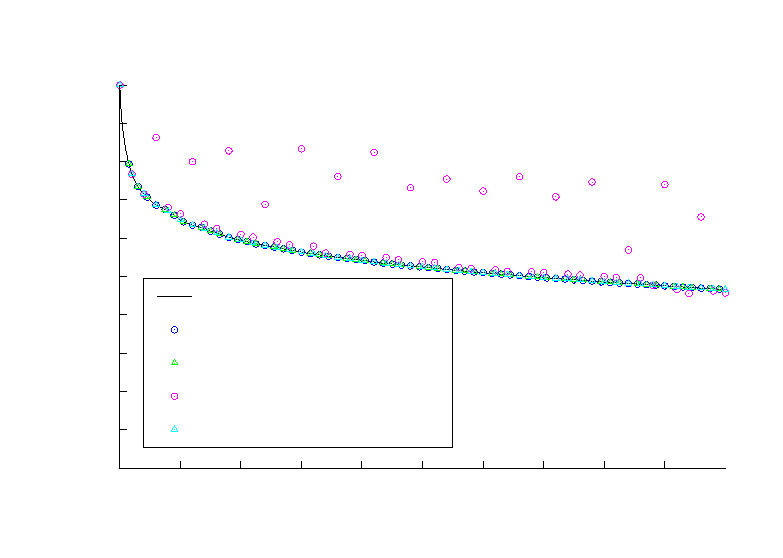
\includegraphics{dmat1}}%
    \gplfronttext
  \end{picture}%
\endgroup
}
	\caption{•••}
	\label{fig:dmat1}
\end{figure}
\begin{figure}
	\centering
	\resizebox{.9\textwidth}{!}{% GNUPLOT: LaTeX picture with Postscript
\begingroup
  \fontfamily{phv}%
  \selectfont
  \makeatletter
  \providecommand\color[2][]{%
    \GenericError{(gnuplot) \space\space\space\@spaces}{%
      Package color not loaded in conjunction with
      terminal option `colourtext'%
    }{See the gnuplot documentation for explanation.%
    }{Either use 'blacktext' in gnuplot or load the package
      color.sty in LaTeX.}%
    \renewcommand\color[2][]{}%
  }%
  \providecommand\includegraphics[2][]{%
    \GenericError{(gnuplot) \space\space\space\@spaces}{%
      Package graphicx or graphics not loaded%
    }{See the gnuplot documentation for explanation.%
    }{The gnuplot epslatex terminal needs graphicx.sty or graphics.sty.}%
    \renewcommand\includegraphics[2][]{}%
  }%
  \providecommand\rotatebox[2]{#2}%
  \@ifundefined{ifGPcolor}{%
    \newif\ifGPcolor
    \GPcolorfalse
  }{}%
  \@ifundefined{ifGPblacktext}{%
    \newif\ifGPblacktext
    \GPblacktexttrue
  }{}%
  % define a \g@addto@macro without @ in the name:
  \let\gplgaddtomacro\g@addto@macro
  % define empty templates for all commands taking text:
  \gdef\gplbacktext{}%
  \gdef\gplfronttext{}%
  \makeatother
  \ifGPblacktext
    % no textcolor at all
    \def\colorrgb#1{}%
    \def\colorgray#1{}%
  \else
    % gray or color?
    \ifGPcolor
      \def\colorrgb#1{\color[rgb]{#1}}%
      \def\colorgray#1{\color[gray]{#1}}%
      \expandafter\def\csname LTw\endcsname{\color{white}}%
      \expandafter\def\csname LTb\endcsname{\color{black}}%
      \expandafter\def\csname LTa\endcsname{\color{black}}%
      \expandafter\def\csname LT0\endcsname{\color[rgb]{1,0,0}}%
      \expandafter\def\csname LT1\endcsname{\color[rgb]{0,1,0}}%
      \expandafter\def\csname LT2\endcsname{\color[rgb]{0,0,1}}%
      \expandafter\def\csname LT3\endcsname{\color[rgb]{1,0,1}}%
      \expandafter\def\csname LT4\endcsname{\color[rgb]{0,1,1}}%
      \expandafter\def\csname LT5\endcsname{\color[rgb]{1,1,0}}%
      \expandafter\def\csname LT6\endcsname{\color[rgb]{0,0,0}}%
      \expandafter\def\csname LT7\endcsname{\color[rgb]{1,0.3,0}}%
      \expandafter\def\csname LT8\endcsname{\color[rgb]{0.5,0.5,0.5}}%
    \else
      % gray
      \def\colorrgb#1{\color{black}}%
      \def\colorgray#1{\color[gray]{#1}}%
      \expandafter\def\csname LTw\endcsname{\color{white}}%
      \expandafter\def\csname LTb\endcsname{\color{black}}%
      \expandafter\def\csname LTa\endcsname{\color{black}}%
      \expandafter\def\csname LT0\endcsname{\color{black}}%
      \expandafter\def\csname LT1\endcsname{\color{black}}%
      \expandafter\def\csname LT2\endcsname{\color{black}}%
      \expandafter\def\csname LT3\endcsname{\color{black}}%
      \expandafter\def\csname LT4\endcsname{\color{black}}%
      \expandafter\def\csname LT5\endcsname{\color{black}}%
      \expandafter\def\csname LT6\endcsname{\color{black}}%
      \expandafter\def\csname LT7\endcsname{\color{black}}%
      \expandafter\def\csname LT8\endcsname{\color{black}}%
    \fi
  \fi
    \setlength{\unitlength}{0.0500bp}%
    \ifx\gptboxheight\undefined%
      \newlength{\gptboxheight}%
      \newlength{\gptboxwidth}%
      \newsavebox{\gptboxtext}%
    \fi%
    \setlength{\fboxrule}{0.5pt}%
    \setlength{\fboxsep}{1pt}%
\begin{picture}(7200.00,5040.00)%
    \gplgaddtomacro\gplbacktext{%
      \csname LTb\endcsname%
      \put(858,704){\makebox(0,0)[r]{\strut{}\footnotesize -10}}%
      \put(858,1072){\makebox(0,0)[r]{\strut{}\footnotesize -9}}%
      \put(858,1439){\makebox(0,0)[r]{\strut{}\footnotesize -8}}%
      \put(858,1807){\makebox(0,0)[r]{\strut{}\footnotesize -7}}%
      \put(858,2174){\makebox(0,0)[r]{\strut{}\footnotesize -6}}%
      \put(858,2542){\makebox(0,0)[r]{\strut{}\footnotesize -5}}%
      \put(858,2909){\makebox(0,0)[r]{\strut{}\footnotesize -4}}%
      \put(858,3277){\makebox(0,0)[r]{\strut{}\footnotesize -3}}%
      \put(858,3644){\makebox(0,0)[r]{\strut{}\footnotesize -2}}%
      \put(858,4012){\makebox(0,0)[r]{\strut{}\footnotesize -1}}%
      \put(858,4379){\makebox(0,0)[r]{\strut{}\footnotesize 0}}%
      \put(1571,484){\makebox(0,0){\strut{}\footnotesize 100}}%
      \put(2153,484){\makebox(0,0){\strut{}\footnotesize 200}}%
      \put(2734,484){\makebox(0,0){\strut{}\footnotesize 300}}%
      \put(3315,484){\makebox(0,0){\strut{}\footnotesize 400}}%
      \put(3897,484){\makebox(0,0){\strut{}\footnotesize 500}}%
      \put(4478,484){\makebox(0,0){\strut{}\footnotesize 600}}%
      \put(5059,484){\makebox(0,0){\strut{}\footnotesize 700}}%
      \put(5640,484){\makebox(0,0){\strut{}\footnotesize 800}}%
      \put(6222,484){\makebox(0,0){\strut{}\footnotesize 900}}%
    }%
    \gplgaddtomacro\gplfronttext{%
      \csname LTb\endcsname%
      \put(352,2541){\rotatebox{-270}{\makebox(0,0){\strut{}\footnotesize Residual 2-norm, log scale}}}%
      \put(3896,154){\makebox(0,0){\strut{}\footnotesize Iteration count}}%
      \put(3896,4709){\makebox(0,0){\strut{}\shortstack{\footnotesize\,1e+04\,times,1e+04\,diagonal,\,logspace\,eigs,\,cond\,1e+10\\\footnotesize\,Residual\,2-norm,\,log\,scale}}}%
      \csname LTb\endcsname%
      \put(1800,2349){\makebox(0,0)[l]{\strut{}\scriptsize GMRES(120)}}%
      \csname LTb\endcsname%
      \put(1800,2030){\makebox(0,0)[l]{\strut{}\begin{minipage}[l]{.95\textwidth} \scriptsize Monomial-GMRES(15,8) \newline \tiny min, max rcond \#: 2.9e-12, 4.6e-12\end{minipage}}}%
      \csname LTb\endcsname%
      \put(1800,1711){\makebox(0,0)[l]{\strut{}\begin{minipage}[l]{.95\textwidth} \scriptsize Newton-GMRES(15,8) \newline \tiny min, max rcond \#: 2.6e-09, 3.4e-09\end{minipage}}}%
      \csname LTb\endcsname%
      \put(1800,1392){\makebox(0,0)[l]{\strut{}\begin{minipage}[l]{.95\textwidth} \scriptsize Monomial-GMRES(20,6) \newline \tiny min, max rcond \#: 3.7e-16, 6.6e-16\end{minipage}}}%
      \csname LTb\endcsname%
      \put(1800,1073){\makebox(0,0)[l]{\strut{}\begin{minipage}[l]{.95\textwidth} \scriptsize Newton-GMRES(20,6) \newline \tiny min, max rcond \#: 2.3e-12, 3.3e-12\end{minipage}}}%
    }%
    \gplbacktext
    \put(0,0){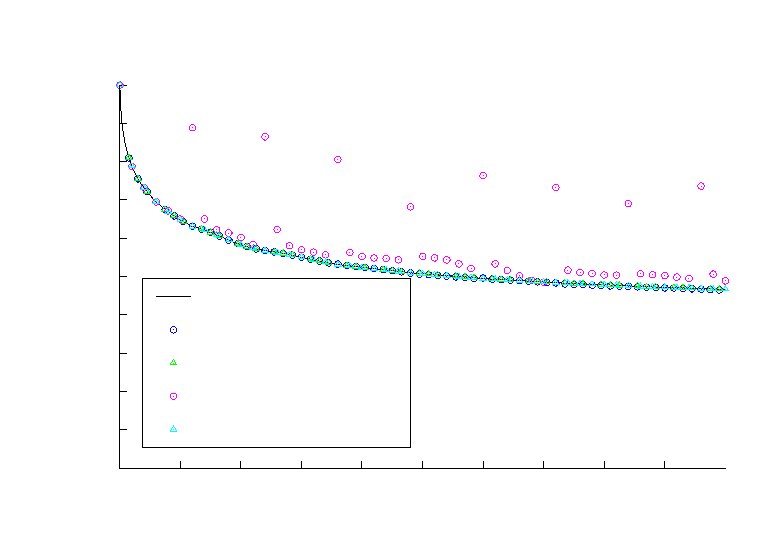
\includegraphics{dmat2}}%
    \gplfronttext
  \end{picture}%
\endgroup
}
	\caption{•••}
	\label{fig:dmat2}
\end{figure}
\begin{figure}
	\centering
	\resizebox{.9\textwidth}{!}{% GNUPLOT: LaTeX picture with Postscript
\begingroup
  \fontfamily{phv}%
  \selectfont
  \makeatletter
  \providecommand\color[2][]{%
    \GenericError{(gnuplot) \space\space\space\@spaces}{%
      Package color not loaded in conjunction with
      terminal option `colourtext'%
    }{See the gnuplot documentation for explanation.%
    }{Either use 'blacktext' in gnuplot or load the package
      color.sty in LaTeX.}%
    \renewcommand\color[2][]{}%
  }%
  \providecommand\includegraphics[2][]{%
    \GenericError{(gnuplot) \space\space\space\@spaces}{%
      Package graphicx or graphics not loaded%
    }{See the gnuplot documentation for explanation.%
    }{The gnuplot epslatex terminal needs graphicx.sty or graphics.sty.}%
    \renewcommand\includegraphics[2][]{}%
  }%
  \providecommand\rotatebox[2]{#2}%
  \@ifundefined{ifGPcolor}{%
    \newif\ifGPcolor
    \GPcolorfalse
  }{}%
  \@ifundefined{ifGPblacktext}{%
    \newif\ifGPblacktext
    \GPblacktexttrue
  }{}%
  % define a \g@addto@macro without @ in the name:
  \let\gplgaddtomacro\g@addto@macro
  % define empty templates for all commands taking text:
  \gdef\gplbacktext{}%
  \gdef\gplfronttext{}%
  \makeatother
  \ifGPblacktext
    % no textcolor at all
    \def\colorrgb#1{}%
    \def\colorgray#1{}%
  \else
    % gray or color?
    \ifGPcolor
      \def\colorrgb#1{\color[rgb]{#1}}%
      \def\colorgray#1{\color[gray]{#1}}%
      \expandafter\def\csname LTw\endcsname{\color{white}}%
      \expandafter\def\csname LTb\endcsname{\color{black}}%
      \expandafter\def\csname LTa\endcsname{\color{black}}%
      \expandafter\def\csname LT0\endcsname{\color[rgb]{1,0,0}}%
      \expandafter\def\csname LT1\endcsname{\color[rgb]{0,1,0}}%
      \expandafter\def\csname LT2\endcsname{\color[rgb]{0,0,1}}%
      \expandafter\def\csname LT3\endcsname{\color[rgb]{1,0,1}}%
      \expandafter\def\csname LT4\endcsname{\color[rgb]{0,1,1}}%
      \expandafter\def\csname LT5\endcsname{\color[rgb]{1,1,0}}%
      \expandafter\def\csname LT6\endcsname{\color[rgb]{0,0,0}}%
      \expandafter\def\csname LT7\endcsname{\color[rgb]{1,0.3,0}}%
      \expandafter\def\csname LT8\endcsname{\color[rgb]{0.5,0.5,0.5}}%
    \else
      % gray
      \def\colorrgb#1{\color{black}}%
      \def\colorgray#1{\color[gray]{#1}}%
      \expandafter\def\csname LTw\endcsname{\color{white}}%
      \expandafter\def\csname LTb\endcsname{\color{black}}%
      \expandafter\def\csname LTa\endcsname{\color{black}}%
      \expandafter\def\csname LT0\endcsname{\color{black}}%
      \expandafter\def\csname LT1\endcsname{\color{black}}%
      \expandafter\def\csname LT2\endcsname{\color{black}}%
      \expandafter\def\csname LT3\endcsname{\color{black}}%
      \expandafter\def\csname LT4\endcsname{\color{black}}%
      \expandafter\def\csname LT5\endcsname{\color{black}}%
      \expandafter\def\csname LT6\endcsname{\color{black}}%
      \expandafter\def\csname LT7\endcsname{\color{black}}%
      \expandafter\def\csname LT8\endcsname{\color{black}}%
    \fi
  \fi
    \setlength{\unitlength}{0.0500bp}%
    \ifx\gptboxheight\undefined%
      \newlength{\gptboxheight}%
      \newlength{\gptboxwidth}%
      \newsavebox{\gptboxtext}%
    \fi%
    \setlength{\fboxrule}{0.5pt}%
    \setlength{\fboxsep}{1pt}%
\begin{picture}(7200.00,5040.00)%
    \gplgaddtomacro\gplbacktext{%
      \csname LTb\endcsname%
      \put(858,704){\makebox(0,0)[r]{\strut{}\footnotesize -10}}%
      \put(858,1072){\makebox(0,0)[r]{\strut{}\footnotesize -9}}%
      \put(858,1439){\makebox(0,0)[r]{\strut{}\footnotesize -8}}%
      \put(858,1807){\makebox(0,0)[r]{\strut{}\footnotesize -7}}%
      \put(858,2174){\makebox(0,0)[r]{\strut{}\footnotesize -6}}%
      \put(858,2542){\makebox(0,0)[r]{\strut{}\footnotesize -5}}%
      \put(858,2909){\makebox(0,0)[r]{\strut{}\footnotesize -4}}%
      \put(858,3277){\makebox(0,0)[r]{\strut{}\footnotesize -3}}%
      \put(858,3644){\makebox(0,0)[r]{\strut{}\footnotesize -2}}%
      \put(858,4012){\makebox(0,0)[r]{\strut{}\footnotesize -1}}%
      \put(858,4379){\makebox(0,0)[r]{\strut{}\footnotesize 0}}%
      \put(1571,484){\makebox(0,0){\strut{}\footnotesize 100}}%
      \put(2153,484){\makebox(0,0){\strut{}\footnotesize 200}}%
      \put(2734,484){\makebox(0,0){\strut{}\footnotesize 300}}%
      \put(3315,484){\makebox(0,0){\strut{}\footnotesize 400}}%
      \put(3897,484){\makebox(0,0){\strut{}\footnotesize 500}}%
      \put(4478,484){\makebox(0,0){\strut{}\footnotesize 600}}%
      \put(5059,484){\makebox(0,0){\strut{}\footnotesize 700}}%
      \put(5640,484){\makebox(0,0){\strut{}\footnotesize 800}}%
      \put(6222,484){\makebox(0,0){\strut{}\footnotesize 900}}%
    }%
    \gplgaddtomacro\gplfronttext{%
      \csname LTb\endcsname%
      \put(352,2541){\rotatebox{-270}{\makebox(0,0){\strut{}\footnotesize Residual 2-norm, log scale}}}%
      \put(3896,154){\makebox(0,0){\strut{}\footnotesize Iteration count}}%
      \put(3896,4709){\makebox(0,0){\strut{}\shortstack{\footnotesize\,1e+04\,times,1e+04\,diagonal,\,logspace\,eigs,\,cond\,1e+15\\\footnotesize\,Residual\,2-norm,\,log\,scale}}}%
      \csname LTb\endcsname%
      \put(1800,2349){\makebox(0,0)[l]{\strut{}\scriptsize GMRES(120)}}%
      \csname LTb\endcsname%
      \put(1800,2030){\makebox(0,0)[l]{\strut{}\begin{minipage}[l]{.95\textwidth} \scriptsize Monomial-GMRES(15,8) \newline \tiny min, max rcond \#: 2.5e-12, 4.4e-12\end{minipage}}}%
      \csname LTb\endcsname%
      \put(1800,1711){\makebox(0,0)[l]{\strut{}\begin{minipage}[l]{.95\textwidth} \scriptsize Newton-GMRES(15,8) \newline \tiny min, max rcond \#: 1.7e-09, 3.5e-09\end{minipage}}}%
      \csname LTb\endcsname%
      \put(1800,1392){\makebox(0,0)[l]{\strut{}\begin{minipage}[l]{.95\textwidth} \scriptsize Monomial-GMRES(20,6) \newline \tiny min, max rcond \#: 2.9e-16, 7.6e-16\end{minipage}}}%
      \csname LTb\endcsname%
      \put(1800,1073){\makebox(0,0)[l]{\strut{}\begin{minipage}[l]{.95\textwidth} \scriptsize Newton-GMRES(20,6) \newline \tiny min, max rcond \#: 1.3e-12, 3.3e-12\end{minipage}}}%
    }%
    \gplbacktext
    \put(0,0){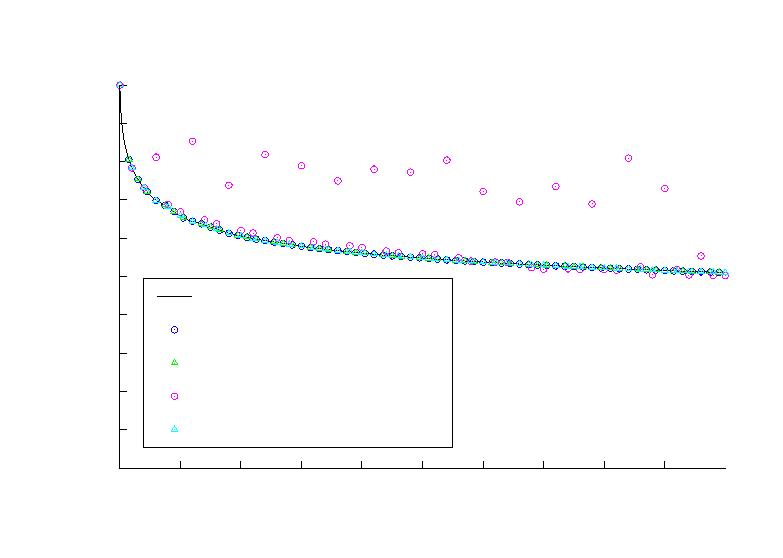
\includegraphics{dmat3}}%
    \gplfronttext
  \end{picture}%
\endgroup
}	
	\caption{•••}
	\label{fig:dmat3}
\end{figure}
\begin{figure}
	\centering
	\resizebox{.9\textwidth}{!}{% GNUPLOT: LaTeX picture with Postscript
\begingroup
  \fontfamily{phv}%
  \selectfont
  \makeatletter
  \providecommand\color[2][]{%
    \GenericError{(gnuplot) \space\space\space\@spaces}{%
      Package color not loaded in conjunction with
      terminal option `colourtext'%
    }{See the gnuplot documentation for explanation.%
    }{Either use 'blacktext' in gnuplot or load the package
      color.sty in LaTeX.}%
    \renewcommand\color[2][]{}%
  }%
  \providecommand\includegraphics[2][]{%
    \GenericError{(gnuplot) \space\space\space\@spaces}{%
      Package graphicx or graphics not loaded%
    }{See the gnuplot documentation for explanation.%
    }{The gnuplot epslatex terminal needs graphicx.sty or graphics.sty.}%
    \renewcommand\includegraphics[2][]{}%
  }%
  \providecommand\rotatebox[2]{#2}%
  \@ifundefined{ifGPcolor}{%
    \newif\ifGPcolor
    \GPcolorfalse
  }{}%
  \@ifundefined{ifGPblacktext}{%
    \newif\ifGPblacktext
    \GPblacktexttrue
  }{}%
  % define a \g@addto@macro without @ in the name:
  \let\gplgaddtomacro\g@addto@macro
  % define empty templates for all commands taking text:
  \gdef\gplbacktext{}%
  \gdef\gplfronttext{}%
  \makeatother
  \ifGPblacktext
    % no textcolor at all
    \def\colorrgb#1{}%
    \def\colorgray#1{}%
  \else
    % gray or color?
    \ifGPcolor
      \def\colorrgb#1{\color[rgb]{#1}}%
      \def\colorgray#1{\color[gray]{#1}}%
      \expandafter\def\csname LTw\endcsname{\color{white}}%
      \expandafter\def\csname LTb\endcsname{\color{black}}%
      \expandafter\def\csname LTa\endcsname{\color{black}}%
      \expandafter\def\csname LT0\endcsname{\color[rgb]{1,0,0}}%
      \expandafter\def\csname LT1\endcsname{\color[rgb]{0,1,0}}%
      \expandafter\def\csname LT2\endcsname{\color[rgb]{0,0,1}}%
      \expandafter\def\csname LT3\endcsname{\color[rgb]{1,0,1}}%
      \expandafter\def\csname LT4\endcsname{\color[rgb]{0,1,1}}%
      \expandafter\def\csname LT5\endcsname{\color[rgb]{1,1,0}}%
      \expandafter\def\csname LT6\endcsname{\color[rgb]{0,0,0}}%
      \expandafter\def\csname LT7\endcsname{\color[rgb]{1,0.3,0}}%
      \expandafter\def\csname LT8\endcsname{\color[rgb]{0.5,0.5,0.5}}%
    \else
      % gray
      \def\colorrgb#1{\color{black}}%
      \def\colorgray#1{\color[gray]{#1}}%
      \expandafter\def\csname LTw\endcsname{\color{white}}%
      \expandafter\def\csname LTb\endcsname{\color{black}}%
      \expandafter\def\csname LTa\endcsname{\color{black}}%
      \expandafter\def\csname LT0\endcsname{\color{black}}%
      \expandafter\def\csname LT1\endcsname{\color{black}}%
      \expandafter\def\csname LT2\endcsname{\color{black}}%
      \expandafter\def\csname LT3\endcsname{\color{black}}%
      \expandafter\def\csname LT4\endcsname{\color{black}}%
      \expandafter\def\csname LT5\endcsname{\color{black}}%
      \expandafter\def\csname LT6\endcsname{\color{black}}%
      \expandafter\def\csname LT7\endcsname{\color{black}}%
      \expandafter\def\csname LT8\endcsname{\color{black}}%
    \fi
  \fi
    \setlength{\unitlength}{0.0500bp}%
    \ifx\gptboxheight\undefined%
      \newlength{\gptboxheight}%
      \newlength{\gptboxwidth}%
      \newsavebox{\gptboxtext}%
    \fi%
    \setlength{\fboxrule}{0.5pt}%
    \setlength{\fboxsep}{1pt}%
\begin{picture}(7200.00,5040.00)%
    \gplgaddtomacro\gplbacktext{%
      \csname LTb\endcsname%
      \put(858,704){\makebox(0,0)[r]{\strut{}\footnotesize -10}}%
      \put(858,1072){\makebox(0,0)[r]{\strut{}\footnotesize -9}}%
      \put(858,1439){\makebox(0,0)[r]{\strut{}\footnotesize -8}}%
      \put(858,1807){\makebox(0,0)[r]{\strut{}\footnotesize -7}}%
      \put(858,2174){\makebox(0,0)[r]{\strut{}\footnotesize -6}}%
      \put(858,2542){\makebox(0,0)[r]{\strut{}\footnotesize -5}}%
      \put(858,2909){\makebox(0,0)[r]{\strut{}\footnotesize -4}}%
      \put(858,3277){\makebox(0,0)[r]{\strut{}\footnotesize -3}}%
      \put(858,3644){\makebox(0,0)[r]{\strut{}\footnotesize -2}}%
      \put(858,4012){\makebox(0,0)[r]{\strut{}\footnotesize -1}}%
      \put(858,4379){\makebox(0,0)[r]{\strut{}\footnotesize 0}}%
      \put(1571,484){\makebox(0,0){\strut{}\footnotesize 100}}%
      \put(2153,484){\makebox(0,0){\strut{}\footnotesize 200}}%
      \put(2734,484){\makebox(0,0){\strut{}\footnotesize 300}}%
      \put(3315,484){\makebox(0,0){\strut{}\footnotesize 400}}%
      \put(3897,484){\makebox(0,0){\strut{}\footnotesize 500}}%
      \put(4478,484){\makebox(0,0){\strut{}\footnotesize 600}}%
      \put(5059,484){\makebox(0,0){\strut{}\footnotesize 700}}%
      \put(5640,484){\makebox(0,0){\strut{}\footnotesize 800}}%
      \put(6222,484){\makebox(0,0){\strut{}\footnotesize 900}}%
			\put(6803,484){\makebox(0,0){\strut{}\footnotesize 1000}}%
    }%
    \gplgaddtomacro\gplfronttext{%
      \csname LTb\endcsname%
      \put(352,2541){\rotatebox{-270}{\makebox(0,0){\strut{}\footnotesize Residual 2-norm, log scale}}}%
      \put(3896,154){\makebox(0,0){\strut{}\footnotesize Iteration count}}%
      \put(3896,4709){\makebox(0,0){\strut{}\shortstack{\footnotesize\,1e+04\,times,1e+04\,diagonal,\,logspace\,eigs,\,cond\,1e+05\\\footnotesize\,Residual\,2-norm,\,log\,scale}}}%
      \csname LTb\endcsname%
      \put(1811,2349){\makebox(0,0)[l]{\strut{}\scriptsize GMRES(60)}}%
      \csname LTb\endcsname%
      \put(1811,2030){\makebox(0,0)[l]{\strut{}\begin{minipage}[l]{.95\textwidth} \scriptsize Monomial-GMRES(15,4) \newline \tiny min, max basis rcond \#: 4.67e-12, 5.19e-12\end{minipage}}}%
      \csname LTb\endcsname%
      \put(1811,1711){\makebox(0,0)[l]{\strut{}\begin{minipage}[l]{.95\textwidth} \scriptsize Newton-GMRES(15,4) \newline \tiny min, max basis rcond \#: 1.84e-02, 3.79e-02\end{minipage}}}%
      \csname LTb\endcsname%
      \put(1811,1392){\makebox(0,0)[l]{\strut{}\begin{minipage}[l]{.95\textwidth} \scriptsize Monomial-GMRES(20,3) \newline \tiny min, max basis rcond \#: 2.18e-16, 7.63e-16\end{minipage}}}%
      \csname LTb\endcsname%
      \put(1811,1073){\makebox(0,0)[l]{\strut{}\begin{minipage}[l]{.95\textwidth} \scriptsize Newton-GMRES(20,3) \newline \tiny min, max basis rcond \#: 8.62e-03, 1.38e-02\end{minipage}}}%
    }%
    \gplbacktext
    \put(0,0){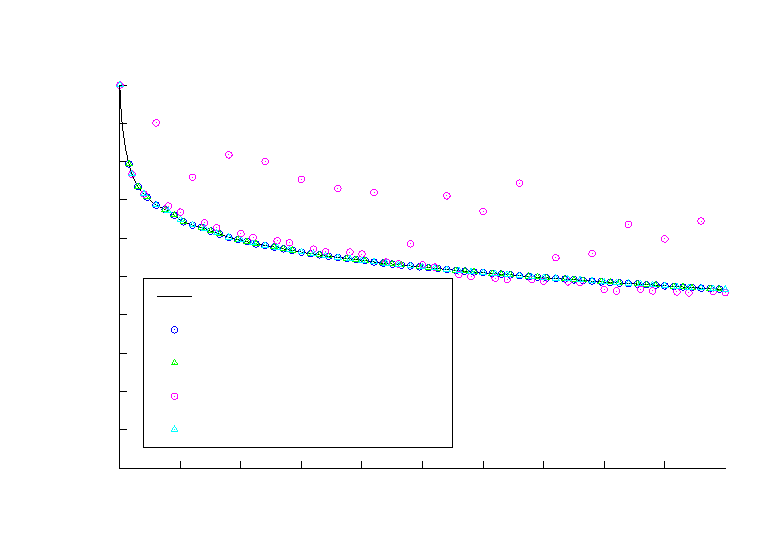
\includegraphics{dmat1_scale}}%
    \gplfronttext
  \end{picture}%
\endgroup
}
	\caption{•••}
	\label{fig:dmat1_scale}
\end{figure}
\begin{figure}
	\centering
	\resizebox{.9\textwidth}{!}{% GNUPLOT: LaTeX picture with Postscript
\begingroup
  \fontfamily{phv}%
  \selectfont
  \makeatletter
  \providecommand\color[2][]{%
    \GenericError{(gnuplot) \space\space\space\@spaces}{%
      Package color not loaded in conjunction with
      terminal option `colourtext'%
    }{See the gnuplot documentation for explanation.%
    }{Either use 'blacktext' in gnuplot or load the package
      color.sty in LaTeX.}%
    \renewcommand\color[2][]{}%
  }%
  \providecommand\includegraphics[2][]{%
    \GenericError{(gnuplot) \space\space\space\@spaces}{%
      Package graphicx or graphics not loaded%
    }{See the gnuplot documentation for explanation.%
    }{The gnuplot epslatex terminal needs graphicx.sty or graphics.sty.}%
    \renewcommand\includegraphics[2][]{}%
  }%
  \providecommand\rotatebox[2]{#2}%
  \@ifundefined{ifGPcolor}{%
    \newif\ifGPcolor
    \GPcolorfalse
  }{}%
  \@ifundefined{ifGPblacktext}{%
    \newif\ifGPblacktext
    \GPblacktexttrue
  }{}%
  % define a \g@addto@macro without @ in the name:
  \let\gplgaddtomacro\g@addto@macro
  % define empty templates for all commands taking text:
  \gdef\gplbacktext{}%
  \gdef\gplfronttext{}%
  \makeatother
  \ifGPblacktext
    % no textcolor at all
    \def\colorrgb#1{}%
    \def\colorgray#1{}%
  \else
    % gray or color?
    \ifGPcolor
      \def\colorrgb#1{\color[rgb]{#1}}%
      \def\colorgray#1{\color[gray]{#1}}%
      \expandafter\def\csname LTw\endcsname{\color{white}}%
      \expandafter\def\csname LTb\endcsname{\color{black}}%
      \expandafter\def\csname LTa\endcsname{\color{black}}%
      \expandafter\def\csname LT0\endcsname{\color[rgb]{1,0,0}}%
      \expandafter\def\csname LT1\endcsname{\color[rgb]{0,1,0}}%
      \expandafter\def\csname LT2\endcsname{\color[rgb]{0,0,1}}%
      \expandafter\def\csname LT3\endcsname{\color[rgb]{1,0,1}}%
      \expandafter\def\csname LT4\endcsname{\color[rgb]{0,1,1}}%
      \expandafter\def\csname LT5\endcsname{\color[rgb]{1,1,0}}%
      \expandafter\def\csname LT6\endcsname{\color[rgb]{0,0,0}}%
      \expandafter\def\csname LT7\endcsname{\color[rgb]{1,0.3,0}}%
      \expandafter\def\csname LT8\endcsname{\color[rgb]{0.5,0.5,0.5}}%
    \else
      % gray
      \def\colorrgb#1{\color{black}}%
      \def\colorgray#1{\color[gray]{#1}}%
      \expandafter\def\csname LTw\endcsname{\color{white}}%
      \expandafter\def\csname LTb\endcsname{\color{black}}%
      \expandafter\def\csname LTa\endcsname{\color{black}}%
      \expandafter\def\csname LT0\endcsname{\color{black}}%
      \expandafter\def\csname LT1\endcsname{\color{black}}%
      \expandafter\def\csname LT2\endcsname{\color{black}}%
      \expandafter\def\csname LT3\endcsname{\color{black}}%
      \expandafter\def\csname LT4\endcsname{\color{black}}%
      \expandafter\def\csname LT5\endcsname{\color{black}}%
      \expandafter\def\csname LT6\endcsname{\color{black}}%
      \expandafter\def\csname LT7\endcsname{\color{black}}%
      \expandafter\def\csname LT8\endcsname{\color{black}}%
    \fi
  \fi
    \setlength{\unitlength}{0.0500bp}%
    \ifx\gptboxheight\undefined%
      \newlength{\gptboxheight}%
      \newlength{\gptboxwidth}%
      \newsavebox{\gptboxtext}%
    \fi%
    \setlength{\fboxrule}{0.5pt}%
    \setlength{\fboxsep}{1pt}%
\begin{picture}(7200.00,5040.00)%
    \gplgaddtomacro\gplbacktext{%
      \csname LTb\endcsname%
      \put(858,704){\makebox(0,0)[r]{\strut{}\footnotesize -10}}%
      \put(858,1072){\makebox(0,0)[r]{\strut{}\footnotesize -9}}%
      \put(858,1439){\makebox(0,0)[r]{\strut{}\footnotesize -8}}%
      \put(858,1807){\makebox(0,0)[r]{\strut{}\footnotesize -7}}%
      \put(858,2174){\makebox(0,0)[r]{\strut{}\footnotesize -6}}%
      \put(858,2542){\makebox(0,0)[r]{\strut{}\footnotesize -5}}%
      \put(858,2909){\makebox(0,0)[r]{\strut{}\footnotesize -4}}%
      \put(858,3277){\makebox(0,0)[r]{\strut{}\footnotesize -3}}%
      \put(858,3644){\makebox(0,0)[r]{\strut{}\footnotesize -2}}%
      \put(858,4012){\makebox(0,0)[r]{\strut{}\footnotesize -1}}%
      \put(858,4379){\makebox(0,0)[r]{\strut{}\footnotesize 0}}%
      \put(1571,484){\makebox(0,0){\strut{}\footnotesize 100}}%
      \put(2153,484){\makebox(0,0){\strut{}\footnotesize 200}}%
      \put(2734,484){\makebox(0,0){\strut{}\footnotesize 300}}%
      \put(3315,484){\makebox(0,0){\strut{}\footnotesize 400}}%
      \put(3897,484){\makebox(0,0){\strut{}\footnotesize 500}}%
      \put(4478,484){\makebox(0,0){\strut{}\footnotesize 600}}%
      \put(5059,484){\makebox(0,0){\strut{}\footnotesize 700}}%
      \put(5640,484){\makebox(0,0){\strut{}\footnotesize 800}}%
      \put(6222,484){\makebox(0,0){\strut{}\footnotesize 900}}%
    }%
    \gplgaddtomacro\gplfronttext{%
      \csname LTb\endcsname%
      \put(352,2541){\rotatebox{-270}{\makebox(0,0){\strut{}\footnotesize Residual 2-norm, log scale}}}%
      \put(3896,154){\makebox(0,0){\strut{}\footnotesize Iteration count}}%
      \put(3896,4709){\makebox(0,0){\strut{}\shortstack{\footnotesize\,1e+04\,times,1e+04\,diagonal,\,logspace\,eigs,\,cond\,1e+10\\\footnotesize\,Residual\,2-norm,\,log\,scale}}}%
      \csname LTb\endcsname%
      \put(1811,2349){\makebox(0,0)[l]{\strut{}\scriptsize GMRES(60)}}%
      \csname LTb\endcsname%
      \put(1811,2030){\makebox(0,0)[l]{\strut{}\begin{minipage}[l]{.95\textwidth} \scriptsize Monomial-GMRES(15,4) \newline \tiny min, max basis rcond \#: 4.56e-12, 5.19e-12\end{minipage}}}%
      \csname LTb\endcsname%
      \put(1811,1711){\makebox(0,0)[l]{\strut{}\begin{minipage}[l]{.95\textwidth} \scriptsize Newton-GMRES(15,4) \newline \tiny min, max basis rcond \#: 1.74e-02, 3.50e-02\end{minipage}}}%
      \csname LTb\endcsname%
      \put(1811,1392){\makebox(0,0)[l]{\strut{}\begin{minipage}[l]{.95\textwidth} \scriptsize Monomial-GMRES(20,3) \newline \tiny min, max basis rcond \#: 2.39e-16, 6.93e-16\end{minipage}}}%
      \csname LTb\endcsname%
      \put(1811,1073){\makebox(0,0)[l]{\strut{}\begin{minipage}[l]{.95\textwidth} \scriptsize Newton-GMRES(20,3) \newline \tiny min, max basis rcond \#: 1.02e-02, 1.77e-02\end{minipage}}}%
    }%
    \gplbacktext
    \put(0,0){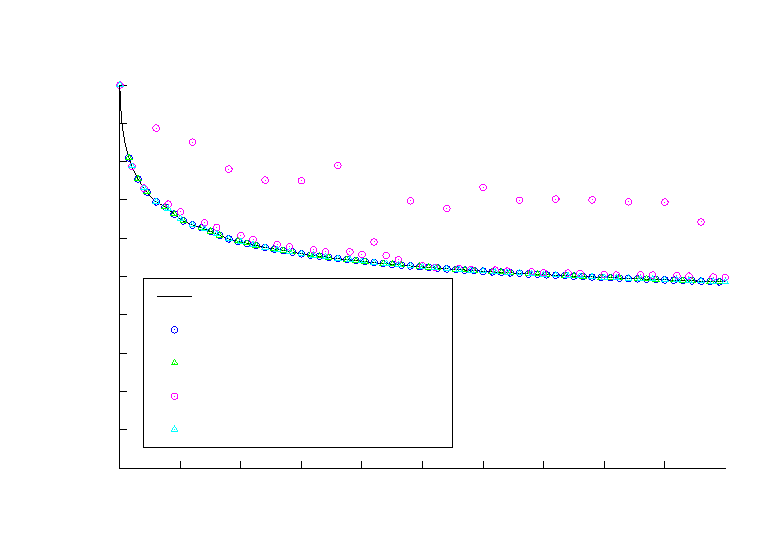
\includegraphics{dmat2_scale}}%
    \gplfronttext
  \end{picture}%
\endgroup
}
	\caption{•••}
	\label{fig:dmat2_scale}
\end{figure}
\begin{figure}
	\centering
	\resizebox{.9\textwidth}{!}{% GNUPLOT: LaTeX picture with Postscript
\begingroup
  \fontfamily{phv}%
  \selectfont
  \makeatletter
  \providecommand\color[2][]{%
    \GenericError{(gnuplot) \space\space\space\@spaces}{%
      Package color not loaded in conjunction with
      terminal option `colourtext'%
    }{See the gnuplot documentation for explanation.%
    }{Either use 'blacktext' in gnuplot or load the package
      color.sty in LaTeX.}%
    \renewcommand\color[2][]{}%
  }%
  \providecommand\includegraphics[2][]{%
    \GenericError{(gnuplot) \space\space\space\@spaces}{%
      Package graphicx or graphics not loaded%
    }{See the gnuplot documentation for explanation.%
    }{The gnuplot epslatex terminal needs graphicx.sty or graphics.sty.}%
    \renewcommand\includegraphics[2][]{}%
  }%
  \providecommand\rotatebox[2]{#2}%
  \@ifundefined{ifGPcolor}{%
    \newif\ifGPcolor
    \GPcolorfalse
  }{}%
  \@ifundefined{ifGPblacktext}{%
    \newif\ifGPblacktext
    \GPblacktexttrue
  }{}%
  % define a \g@addto@macro without @ in the name:
  \let\gplgaddtomacro\g@addto@macro
  % define empty templates for all commands taking text:
  \gdef\gplbacktext{}%
  \gdef\gplfronttext{}%
  \makeatother
  \ifGPblacktext
    % no textcolor at all
    \def\colorrgb#1{}%
    \def\colorgray#1{}%
  \else
    % gray or color?
    \ifGPcolor
      \def\colorrgb#1{\color[rgb]{#1}}%
      \def\colorgray#1{\color[gray]{#1}}%
      \expandafter\def\csname LTw\endcsname{\color{white}}%
      \expandafter\def\csname LTb\endcsname{\color{black}}%
      \expandafter\def\csname LTa\endcsname{\color{black}}%
      \expandafter\def\csname LT0\endcsname{\color[rgb]{1,0,0}}%
      \expandafter\def\csname LT1\endcsname{\color[rgb]{0,1,0}}%
      \expandafter\def\csname LT2\endcsname{\color[rgb]{0,0,1}}%
      \expandafter\def\csname LT3\endcsname{\color[rgb]{1,0,1}}%
      \expandafter\def\csname LT4\endcsname{\color[rgb]{0,1,1}}%
      \expandafter\def\csname LT5\endcsname{\color[rgb]{1,1,0}}%
      \expandafter\def\csname LT6\endcsname{\color[rgb]{0,0,0}}%
      \expandafter\def\csname LT7\endcsname{\color[rgb]{1,0.3,0}}%
      \expandafter\def\csname LT8\endcsname{\color[rgb]{0.5,0.5,0.5}}%
    \else
      % gray
      \def\colorrgb#1{\color{black}}%
      \def\colorgray#1{\color[gray]{#1}}%
      \expandafter\def\csname LTw\endcsname{\color{white}}%
      \expandafter\def\csname LTb\endcsname{\color{black}}%
      \expandafter\def\csname LTa\endcsname{\color{black}}%
      \expandafter\def\csname LT0\endcsname{\color{black}}%
      \expandafter\def\csname LT1\endcsname{\color{black}}%
      \expandafter\def\csname LT2\endcsname{\color{black}}%
      \expandafter\def\csname LT3\endcsname{\color{black}}%
      \expandafter\def\csname LT4\endcsname{\color{black}}%
      \expandafter\def\csname LT5\endcsname{\color{black}}%
      \expandafter\def\csname LT6\endcsname{\color{black}}%
      \expandafter\def\csname LT7\endcsname{\color{black}}%
      \expandafter\def\csname LT8\endcsname{\color{black}}%
    \fi
  \fi
    \setlength{\unitlength}{0.0500bp}%
    \ifx\gptboxheight\undefined%
      \newlength{\gptboxheight}%
      \newlength{\gptboxwidth}%
      \newsavebox{\gptboxtext}%
    \fi%
    \setlength{\fboxrule}{0.5pt}%
    \setlength{\fboxsep}{1pt}%
\begin{picture}(7200.00,5040.00)%
    \gplgaddtomacro\gplbacktext{%
      \csname LTb\endcsname%
      \put(858,704){\makebox(0,0)[r]{\strut{}\footnotesize -10}}%
      \put(858,1072){\makebox(0,0)[r]{\strut{}\footnotesize -9}}%
      \put(858,1439){\makebox(0,0)[r]{\strut{}\footnotesize -8}}%
      \put(858,1807){\makebox(0,0)[r]{\strut{}\footnotesize -7}}%
      \put(858,2174){\makebox(0,0)[r]{\strut{}\footnotesize -6}}%
      \put(858,2542){\makebox(0,0)[r]{\strut{}\footnotesize -5}}%
      \put(858,2909){\makebox(0,0)[r]{\strut{}\footnotesize -4}}%
      \put(858,3277){\makebox(0,0)[r]{\strut{}\footnotesize -3}}%
      \put(858,3644){\makebox(0,0)[r]{\strut{}\footnotesize -2}}%
      \put(858,4012){\makebox(0,0)[r]{\strut{}\footnotesize -1}}%
      \put(858,4379){\makebox(0,0)[r]{\strut{}\footnotesize 0}}%
      \put(1571,484){\makebox(0,0){\strut{}\footnotesize 100}}%
      \put(2153,484){\makebox(0,0){\strut{}\footnotesize 200}}%
      \put(2734,484){\makebox(0,0){\strut{}\footnotesize 300}}%
      \put(3315,484){\makebox(0,0){\strut{}\footnotesize 400}}%
      \put(3897,484){\makebox(0,0){\strut{}\footnotesize 500}}%
      \put(4478,484){\makebox(0,0){\strut{}\footnotesize 600}}%
      \put(5059,484){\makebox(0,0){\strut{}\footnotesize 700}}%
      \put(5640,484){\makebox(0,0){\strut{}\footnotesize 800}}%
      \put(6222,484){\makebox(0,0){\strut{}\footnotesize 900}}%
			\put(6803,484){\makebox(0,0){\strut{}\footnotesize 1000}}%
    }%
    \gplgaddtomacro\gplfronttext{%
      \csname LTb\endcsname%
      \put(352,2541){\rotatebox{-270}{\makebox(0,0){\strut{}\footnotesize Residual 2-norm, log scale}}}%
      \put(3896,154){\makebox(0,0){\strut{}\footnotesize Iteration count}}%
      \put(3896,4709){\makebox(0,0){\strut{}\shortstack{\footnotesize\,1e+04\,times,1e+04\,diagonal,\,logspace\,eigs,\,cond\,1e+15\\\footnotesize\,Residual\,2-norm,\,log\,scale}}}%
      \csname LTb\endcsname%
      \put(1811,2349){\makebox(0,0)[l]{\strut{}\scriptsize GMRES(60)}}%
      \csname LTb\endcsname%
      \put(1811,2030){\makebox(0,0)[l]{\strut{}\begin{minipage}[l]{.95\textwidth} \scriptsize Monomial-GMRES(15,4) \newline \tiny min, max basis rcond \#: 4.39e-12, 5.34e-12\end{minipage}}}%
      \csname LTb\endcsname%
      \put(1811,1711){\makebox(0,0)[l]{\strut{}\begin{minipage}[l]{.95\textwidth} \scriptsize Newton-GMRES(15,4) \newline \tiny min, max basis rcond \#: 1.66e-02, 3.93e-02\end{minipage}}}%
      \csname LTb\endcsname%
      \put(1811,1392){\makebox(0,0)[l]{\strut{}\begin{minipage}[l]{.95\textwidth} \scriptsize Monomial-GMRES(20,3) \newline \tiny min, max basis rcond \#: 1.24e-16, 6.65e-16\end{minipage}}}%
      \csname LTb\endcsname%
      \put(1811,1073){\makebox(0,0)[l]{\strut{}\begin{minipage}[l]{.95\textwidth} \scriptsize Newton-GMRES(20,3) \newline \tiny min, max basis rcond \#: 1.01e-02, 1.58e-02\end{minipage}}}%
    }%
    \gplbacktext
    \put(0,0){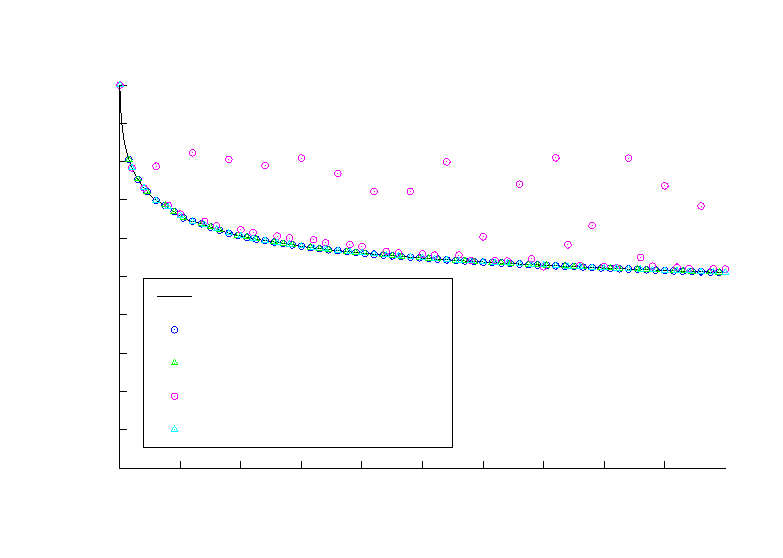
\includegraphics{dmat3_scale}}%
    \gplfronttext
  \end{picture}%
\endgroup
}
	\caption{•••}
	\label{fig:dmat3_scale}
\end{figure}
\begin{figure}
	\centering
	\resizebox{.9\textwidth}{!}{% GNUPLOT: LaTeX picture with Postscript
\begingroup
  \fontfamily{phv}%
  \selectfont
  \makeatletter
  \providecommand\color[2][]{%
    \GenericError{(gnuplot) \space\space\space\@spaces}{%
      Package color not loaded in conjunction with
      terminal option `colourtext'%
    }{See the gnuplot documentation for explanation.%
    }{Either use 'blacktext' in gnuplot or load the package
      color.sty in LaTeX.}%
    \renewcommand\color[2][]{}%
  }%
  \providecommand\includegraphics[2][]{%
    \GenericError{(gnuplot) \space\space\space\@spaces}{%
      Package graphicx or graphics not loaded%
    }{See the gnuplot documentation for explanation.%
    }{The gnuplot epslatex terminal needs graphicx.sty or graphics.sty.}%
    \renewcommand\includegraphics[2][]{}%
  }%
  \providecommand\rotatebox[2]{#2}%
  \@ifundefined{ifGPcolor}{%
    \newif\ifGPcolor
    \GPcolorfalse
  }{}%
  \@ifundefined{ifGPblacktext}{%
    \newif\ifGPblacktext
    \GPblacktexttrue
  }{}%
  % define a \g@addto@macro without @ in the name:
  \let\gplgaddtomacro\g@addto@macro
  % define empty templates for all commands taking text:
  \gdef\gplbacktext{}%
  \gdef\gplfronttext{}%
  \makeatother
  \ifGPblacktext
    % no textcolor at all
    \def\colorrgb#1{}%
    \def\colorgray#1{}%
  \else
    % gray or color?
    \ifGPcolor
      \def\colorrgb#1{\color[rgb]{#1}}%
      \def\colorgray#1{\color[gray]{#1}}%
      \expandafter\def\csname LTw\endcsname{\color{white}}%
      \expandafter\def\csname LTb\endcsname{\color{black}}%
      \expandafter\def\csname LTa\endcsname{\color{black}}%
      \expandafter\def\csname LT0\endcsname{\color[rgb]{1,0,0}}%
      \expandafter\def\csname LT1\endcsname{\color[rgb]{0,1,0}}%
      \expandafter\def\csname LT2\endcsname{\color[rgb]{0,0,1}}%
      \expandafter\def\csname LT3\endcsname{\color[rgb]{1,0,1}}%
      \expandafter\def\csname LT4\endcsname{\color[rgb]{0,1,1}}%
      \expandafter\def\csname LT5\endcsname{\color[rgb]{1,1,0}}%
      \expandafter\def\csname LT6\endcsname{\color[rgb]{0,0,0}}%
      \expandafter\def\csname LT7\endcsname{\color[rgb]{1,0.3,0}}%
      \expandafter\def\csname LT8\endcsname{\color[rgb]{0.5,0.5,0.5}}%
    \else
      % gray
      \def\colorrgb#1{\color{black}}%
      \def\colorgray#1{\color[gray]{#1}}%
      \expandafter\def\csname LTw\endcsname{\color{white}}%
      \expandafter\def\csname LTb\endcsname{\color{black}}%
      \expandafter\def\csname LTa\endcsname{\color{black}}%
      \expandafter\def\csname LT0\endcsname{\color{black}}%
      \expandafter\def\csname LT1\endcsname{\color{black}}%
      \expandafter\def\csname LT2\endcsname{\color{black}}%
      \expandafter\def\csname LT3\endcsname{\color{black}}%
      \expandafter\def\csname LT4\endcsname{\color{black}}%
      \expandafter\def\csname LT5\endcsname{\color{black}}%
      \expandafter\def\csname LT6\endcsname{\color{black}}%
      \expandafter\def\csname LT7\endcsname{\color{black}}%
      \expandafter\def\csname LT8\endcsname{\color{black}}%
    \fi
  \fi
    \setlength{\unitlength}{0.0500bp}%
    \ifx\gptboxheight\undefined%
      \newlength{\gptboxheight}%
      \newlength{\gptboxwidth}%
      \newsavebox{\gptboxtext}%
    \fi%
    \setlength{\fboxrule}{0.5pt}%
    \setlength{\fboxsep}{1pt}%
\begin{picture}(7200.00,5040.00)%
    \gplgaddtomacro\gplbacktext{%
      \csname LTb\endcsname%
      \put(858,704){\makebox(0,0)[r]{\strut{}\footnotesize -16}}%
      \put(858,1163){\makebox(0,0)[r]{\strut{}\footnotesize -14}}%
      \put(858,1623){\makebox(0,0)[r]{\strut{}\footnotesize -12}}%
      \put(858,2082){\makebox(0,0)[r]{\strut{}\footnotesize -10}}%
      \put(858,2542){\makebox(0,0)[r]{\strut{}\footnotesize -8}}%
      \put(858,3001){\makebox(0,0)[r]{\strut{}\footnotesize -6}}%
      \put(858,3460){\makebox(0,0)[r]{\strut{}\footnotesize -4}}%
      \put(858,3920){\makebox(0,0)[r]{\strut{}\footnotesize -2}}%
      \put(858,4379){\makebox(0,0)[r]{\strut{}\footnotesize 0}}%
      \put(1571,484){\makebox(0,0){\strut{}\footnotesize 100}}%
      \put(2153,484){\makebox(0,0){\strut{}\footnotesize 200}}%
      \put(2734,484){\makebox(0,0){\strut{}\footnotesize 300}}%
      \put(3315,484){\makebox(0,0){\strut{}\footnotesize 400}}%
      \put(3897,484){\makebox(0,0){\strut{}\footnotesize 500}}%
      \put(4478,484){\makebox(0,0){\strut{}\footnotesize 600}}%
      \put(5059,484){\makebox(0,0){\strut{}\footnotesize 700}}%
      \put(5640,484){\makebox(0,0){\strut{}\footnotesize 800}}%
      \put(6222,484){\makebox(0,0){\strut{}\footnotesize 900}}%
			\put(6803,484){\makebox(0,0){\strut{}\footnotesize 1000}}%
    }%
    \gplgaddtomacro\gplfronttext{%
      \csname LTb\endcsname%
      \put(352,2541){\rotatebox{-270}{\makebox(0,0){\strut{}\footnotesize Residual 2-norm, log scale}}}%
      \put(3896,154){\makebox(0,0){\strut{}\footnotesize Iteration count}}%
      \put(3896,4709){\makebox(0,0){\strut{}\shortstack{Watt1}}}%
      \csname LTb\endcsname%
      \put(4311,4192){\makebox(0,0)[l]{\strut{}\scriptsize GMRES(30)}}%
      \csname LTb\endcsname%
      \put(4311,3873){\makebox(0,0)[l]{\strut{}\begin{minipage}[l]{.95\textwidth} \scriptsize Monomial-GMRES(3,10) \newline \tiny min, max basis rcond \#: 9.80e-15, 2.99e-08\end{minipage}}}%
      \csname LTb\endcsname%
      \put(4311,3554){\makebox(0,0)[l]{\strut{}\begin{minipage}[l]{.95\textwidth} \scriptsize Newton-GMRES(3,10) \newline \tiny min, max basis rcond \#: 1.05e-13, 2.11e-07\end{minipage}}}%
      \csname LTb\endcsname%
      \put(4311,3235){\makebox(0,0)[l]{\strut{}\begin{minipage}[l]{.95\textwidth} \scriptsize Monomial-GMRES(5,6) \newline \tiny min, max basis rcond \#: 2.94e-17, 8.57e-11\end{minipage}}}%
      \csname LTb\endcsname%
      \put(4311,2916){\makebox(0,0)[l]{\strut{}\begin{minipage}[l]{.95\textwidth} \scriptsize Newton-GMRES(5,6) \newline \tiny min, max basis rcond \#: 2.71e-25, 4.17e-14\end{minipage}}}%
    }%
    \gplbacktext
    \put(0,0){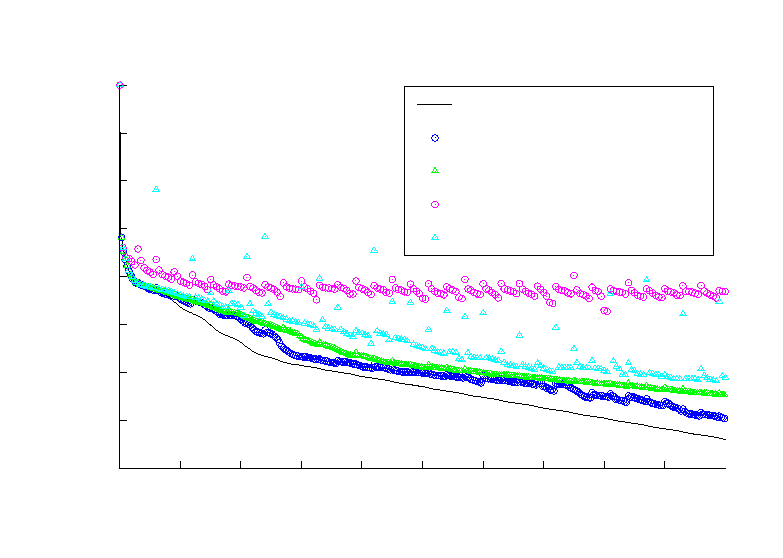
\includegraphics{watt1_noscale}}%
    \gplfronttext
  \end{picture}%
\endgroup
}
	\caption{not scaled}
	\label{fig:watt1_noscale}
\end{figure}
\begin{figure}
	\centering
	\resizebox{.9\textwidth}{!}{% GNUPLOT: LaTeX picture with Postscript
\begingroup
  \fontfamily{phv}%
  \selectfont
  \makeatletter
  \providecommand\color[2][]{%
    \GenericError{(gnuplot) \space\space\space\@spaces}{%
      Package color not loaded in conjunction with
      terminal option `colourtext'%
    }{See the gnuplot documentation for explanation.%
    }{Either use 'blacktext' in gnuplot or load the package
      color.sty in LaTeX.}%
    \renewcommand\color[2][]{}%
  }%
  \providecommand\includegraphics[2][]{%
    \GenericError{(gnuplot) \space\space\space\@spaces}{%
      Package graphicx or graphics not loaded%
    }{See the gnuplot documentation for explanation.%
    }{The gnuplot epslatex terminal needs graphicx.sty or graphics.sty.}%
    \renewcommand\includegraphics[2][]{}%
  }%
  \providecommand\rotatebox[2]{#2}%
  \@ifundefined{ifGPcolor}{%
    \newif\ifGPcolor
    \GPcolorfalse
  }{}%
  \@ifundefined{ifGPblacktext}{%
    \newif\ifGPblacktext
    \GPblacktexttrue
  }{}%
  % define a \g@addto@macro without @ in the name:
  \let\gplgaddtomacro\g@addto@macro
  % define empty templates for all commands taking text:
  \gdef\gplbacktext{}%
  \gdef\gplfronttext{}%
  \makeatother
  \ifGPblacktext
    % no textcolor at all
    \def\colorrgb#1{}%
    \def\colorgray#1{}%
  \else
    % gray or color?
    \ifGPcolor
      \def\colorrgb#1{\color[rgb]{#1}}%
      \def\colorgray#1{\color[gray]{#1}}%
      \expandafter\def\csname LTw\endcsname{\color{white}}%
      \expandafter\def\csname LTb\endcsname{\color{black}}%
      \expandafter\def\csname LTa\endcsname{\color{black}}%
      \expandafter\def\csname LT0\endcsname{\color[rgb]{1,0,0}}%
      \expandafter\def\csname LT1\endcsname{\color[rgb]{0,1,0}}%
      \expandafter\def\csname LT2\endcsname{\color[rgb]{0,0,1}}%
      \expandafter\def\csname LT3\endcsname{\color[rgb]{1,0,1}}%
      \expandafter\def\csname LT4\endcsname{\color[rgb]{0,1,1}}%
      \expandafter\def\csname LT5\endcsname{\color[rgb]{1,1,0}}%
      \expandafter\def\csname LT6\endcsname{\color[rgb]{0,0,0}}%
      \expandafter\def\csname LT7\endcsname{\color[rgb]{1,0.3,0}}%
      \expandafter\def\csname LT8\endcsname{\color[rgb]{0.5,0.5,0.5}}%
    \else
      % gray
      \def\colorrgb#1{\color{black}}%
      \def\colorgray#1{\color[gray]{#1}}%
      \expandafter\def\csname LTw\endcsname{\color{white}}%
      \expandafter\def\csname LTb\endcsname{\color{black}}%
      \expandafter\def\csname LTa\endcsname{\color{black}}%
      \expandafter\def\csname LT0\endcsname{\color{black}}%
      \expandafter\def\csname LT1\endcsname{\color{black}}%
      \expandafter\def\csname LT2\endcsname{\color{black}}%
      \expandafter\def\csname LT3\endcsname{\color{black}}%
      \expandafter\def\csname LT4\endcsname{\color{black}}%
      \expandafter\def\csname LT5\endcsname{\color{black}}%
      \expandafter\def\csname LT6\endcsname{\color{black}}%
      \expandafter\def\csname LT7\endcsname{\color{black}}%
      \expandafter\def\csname LT8\endcsname{\color{black}}%
    \fi
  \fi
    \setlength{\unitlength}{0.0500bp}%
    \ifx\gptboxheight\undefined%
      \newlength{\gptboxheight}%
      \newlength{\gptboxwidth}%
      \newsavebox{\gptboxtext}%
    \fi%
    \setlength{\fboxrule}{0.5pt}%
    \setlength{\fboxsep}{1pt}%
\begin{picture}(7200.00,5040.00)%
    \gplgaddtomacro\gplbacktext{%
      \csname LTb\endcsname%
      \put(858,704){\makebox(0,0)[r]{\strut{}\footnotesize -16}}%
      \put(858,1163){\makebox(0,0)[r]{\strut{}\footnotesize -14}}%
      \put(858,1623){\makebox(0,0)[r]{\strut{}\footnotesize -12}}%
      \put(858,2082){\makebox(0,0)[r]{\strut{}\footnotesize -10}}%
      \put(858,2542){\makebox(0,0)[r]{\strut{}\footnotesize -8}}%
      \put(858,3001){\makebox(0,0)[r]{\strut{}\footnotesize -6}}%
      \put(858,3460){\makebox(0,0)[r]{\strut{}\footnotesize -4}}%
      \put(858,3920){\makebox(0,0)[r]{\strut{}\footnotesize -2}}%
      \put(858,4379){\makebox(0,0)[r]{\strut{}\footnotesize 0}}%
      \put(1571,484){\makebox(0,0){\strut{}\footnotesize 100}}%
      \put(2153,484){\makebox(0,0){\strut{}\footnotesize 200}}%
      \put(2734,484){\makebox(0,0){\strut{}\footnotesize 300}}%
      \put(3315,484){\makebox(0,0){\strut{}\footnotesize 400}}%
      \put(3897,484){\makebox(0,0){\strut{}\footnotesize 500}}%
      \put(4478,484){\makebox(0,0){\strut{}\footnotesize 600}}%
      \put(5059,484){\makebox(0,0){\strut{}\footnotesize 700}}%
      \put(5640,484){\makebox(0,0){\strut{}\footnotesize 800}}%
      \put(6222,484){\makebox(0,0){\strut{}\footnotesize 900}}%
			\put(6803,484){\makebox(0,0){\strut{}\footnotesize 1000}}%
    }%
    \gplgaddtomacro\gplfronttext{%
      \csname LTb\endcsname%
      \put(352,2541){\rotatebox{-270}{\makebox(0,0){\strut{}\footnotesize Residual 2-norm, log scale}}}%
      \put(3896,154){\makebox(0,0){\strut{}\footnotesize Iteration count}}%
      \put(3896,4709){\makebox(0,0){\strut{}\shortstack{Watt1}}}%
      \csname LTb\endcsname%
      \put(4311,4192){\makebox(0,0)[l]{\strut{}\scriptsize GMRES(30)}}%
      \csname LTb\endcsname%
      \put(4311,3873){\makebox(0,0)[l]{\strut{}\begin{minipage}[l]{.95\textwidth} \scriptsize Monomial-GMRES(5,6) \newline \tiny min, max basis rcond \#: 3.62e-17, 6.40e-11\end{minipage}}}%
      \csname LTb\endcsname%
      \put(4311,3554){\makebox(0,0)[l]{\strut{}\begin{minipage}[l]{.95\textwidth} \scriptsize Newton-GMRES(5,6) \newline \tiny min, max basis rcond \#: 1.15e-16, 1.44e-01\end{minipage}}}%
      \csname LTb\endcsname%
      \put(4311,3235){\makebox(0,0)[l]{\strut{}\begin{minipage}[l]{.95\textwidth} \scriptsize Monomial-GMRES(6,5) \newline \tiny min, max basis rcond \#: 2.41e-17, 3.54e-11\end{minipage}}}%
      \csname LTb\endcsname%
      \put(4311,2916){\makebox(0,0)[l]{\strut{}\begin{minipage}[l]{.95\textwidth} \scriptsize Newton-GMRES(6,5) \newline \tiny min, max basis rcond \#: 1.19e-14, 1.61e-02\end{minipage}}}%
    }%
    \gplbacktext
    \put(0,0){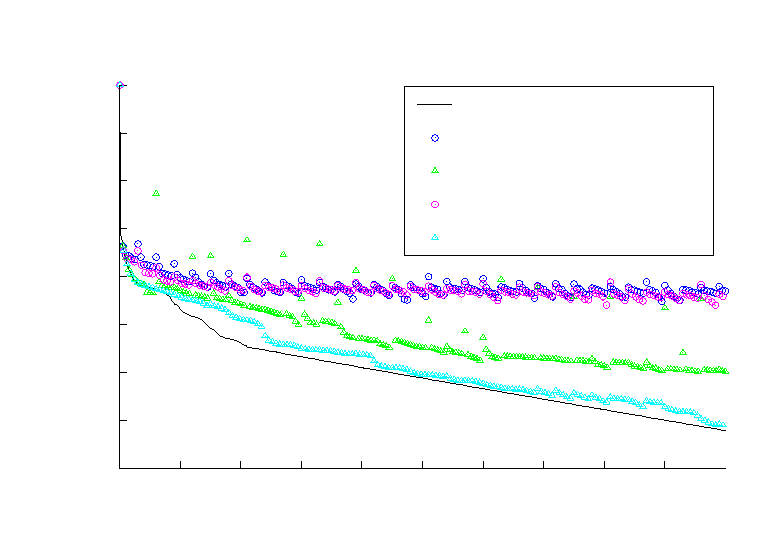
\includegraphics{watt1_scale}}%
    \gplfronttext
  \end{picture}%
\endgroup
}
	\caption{•••}
	\label{fig:watt1_scale}
\end{figure}
\begin{figure}
	\centering
	\resizebox{.9\textwidth}{!}{% GNUPLOT: LaTeX picture with Postscript
\begingroup
  \fontfamily{phv}%
  \selectfont
  \makeatletter
  \providecommand\color[2][]{%
    \GenericError{(gnuplot) \space\space\space\@spaces}{%
      Package color not loaded in conjunction with
      terminal option `colourtext'%
    }{See the gnuplot documentation for explanation.%
    }{Either use 'blacktext' in gnuplot or load the package
      color.sty in LaTeX.}%
    \renewcommand\color[2][]{}%
  }%
  \providecommand\includegraphics[2][]{%
    \GenericError{(gnuplot) \space\space\space\@spaces}{%
      Package graphicx or graphics not loaded%
    }{See the gnuplot documentation for explanation.%
    }{The gnuplot epslatex terminal needs graphicx.sty or graphics.sty.}%
    \renewcommand\includegraphics[2][]{}%
  }%
  \providecommand\rotatebox[2]{#2}%
  \@ifundefined{ifGPcolor}{%
    \newif\ifGPcolor
    \GPcolorfalse
  }{}%
  \@ifundefined{ifGPblacktext}{%
    \newif\ifGPblacktext
    \GPblacktexttrue
  }{}%
  % define a \g@addto@macro without @ in the name:
  \let\gplgaddtomacro\g@addto@macro
  % define empty templates for all commands taking text:
  \gdef\gplbacktext{}%
  \gdef\gplfronttext{}%
  \makeatother
  \ifGPblacktext
    % no textcolor at all
    \def\colorrgb#1{}%
    \def\colorgray#1{}%
  \else
    % gray or color?
    \ifGPcolor
      \def\colorrgb#1{\color[rgb]{#1}}%
      \def\colorgray#1{\color[gray]{#1}}%
      \expandafter\def\csname LTw\endcsname{\color{white}}%
      \expandafter\def\csname LTb\endcsname{\color{black}}%
      \expandafter\def\csname LTa\endcsname{\color{black}}%
      \expandafter\def\csname LT0\endcsname{\color[rgb]{1,0,0}}%
      \expandafter\def\csname LT1\endcsname{\color[rgb]{0,1,0}}%
      \expandafter\def\csname LT2\endcsname{\color[rgb]{0,0,1}}%
      \expandafter\def\csname LT3\endcsname{\color[rgb]{1,0,1}}%
      \expandafter\def\csname LT4\endcsname{\color[rgb]{0,1,1}}%
      \expandafter\def\csname LT5\endcsname{\color[rgb]{1,1,0}}%
      \expandafter\def\csname LT6\endcsname{\color[rgb]{0,0,0}}%
      \expandafter\def\csname LT7\endcsname{\color[rgb]{1,0.3,0}}%
      \expandafter\def\csname LT8\endcsname{\color[rgb]{0.5,0.5,0.5}}%
    \else
      % gray
      \def\colorrgb#1{\color{black}}%
      \def\colorgray#1{\color[gray]{#1}}%
      \expandafter\def\csname LTw\endcsname{\color{white}}%
      \expandafter\def\csname LTb\endcsname{\color{black}}%
      \expandafter\def\csname LTa\endcsname{\color{black}}%
      \expandafter\def\csname LT0\endcsname{\color{black}}%
      \expandafter\def\csname LT1\endcsname{\color{black}}%
      \expandafter\def\csname LT2\endcsname{\color{black}}%
      \expandafter\def\csname LT3\endcsname{\color{black}}%
      \expandafter\def\csname LT4\endcsname{\color{black}}%
      \expandafter\def\csname LT5\endcsname{\color{black}}%
      \expandafter\def\csname LT6\endcsname{\color{black}}%
      \expandafter\def\csname LT7\endcsname{\color{black}}%
      \expandafter\def\csname LT8\endcsname{\color{black}}%
    \fi
  \fi
    \setlength{\unitlength}{0.0500bp}%
    \ifx\gptboxheight\undefined%
      \newlength{\gptboxheight}%
      \newlength{\gptboxwidth}%
      \newsavebox{\gptboxtext}%
    \fi%
    \setlength{\fboxrule}{0.5pt}%
    \setlength{\fboxsep}{1pt}%
\begin{picture}(7200.00,5040.00)%
    \gplgaddtomacro\gplbacktext{%
      \csname LTb\endcsname%
      \put(858,704){\makebox(0,0)[r]{\strut{}\footnotesize -16}}%
      \put(858,1163){\makebox(0,0)[r]{\strut{}\footnotesize -14}}%
      \put(858,1623){\makebox(0,0)[r]{\strut{}\footnotesize -12}}%
      \put(858,2082){\makebox(0,0)[r]{\strut{}\footnotesize -10}}%
      \put(858,2542){\makebox(0,0)[r]{\strut{}\footnotesize -8}}%
      \put(858,3001){\makebox(0,0)[r]{\strut{}\footnotesize -6}}%
      \put(858,3460){\makebox(0,0)[r]{\strut{}\footnotesize -4}}%
      \put(858,3920){\makebox(0,0)[r]{\strut{}\footnotesize -2}}%
      \put(858,4379){\makebox(0,0)[r]{\strut{}\footnotesize 0}}%
      \put(1571,484){\makebox(0,0){\strut{}\footnotesize 100}}%
      \put(2153,484){\makebox(0,0){\strut{}\footnotesize 200}}%
      \put(2734,484){\makebox(0,0){\strut{}\footnotesize 300}}%
      \put(3315,484){\makebox(0,0){\strut{}\footnotesize 400}}%
      \put(3897,484){\makebox(0,0){\strut{}\footnotesize 500}}%
      \put(4478,484){\makebox(0,0){\strut{}\footnotesize 600}}%
      \put(5059,484){\makebox(0,0){\strut{}\footnotesize 700}}%
      \put(5640,484){\makebox(0,0){\strut{}\footnotesize 800}}%
      \put(6222,484){\makebox(0,0){\strut{}\footnotesize 900}}%
      \put(6803,484){\makebox(0,0){\strut{}\footnotesize 1000}}%
    }%
    \gplgaddtomacro\gplfronttext{%
      \csname LTb\endcsname%
      \put(352,2541){\rotatebox{-270}{\makebox(0,0){\strut{}\footnotesize Residual 2-norm, log scale}}}%
      \put(3896,154){\makebox(0,0){\strut{}\footnotesize Iteration count}}%
      \put(3896,4709){\makebox(0,0){\strut{}\shortstack{Watt1}}}%
      \csname LTb\endcsname%
      \put(3783,3973){\makebox(0,0)[l]{\strut{}\scriptsize GMRES(30) + ilu(0)}}%
      \csname LTb\endcsname%
      \put(3783,3654){\makebox(0,0)[l]{\strut{}\begin{minipage}[l]{.95\textwidth} \scriptsize Monomial-GMRES(5,6) + ilu(0) \newline \tiny min, max basis rcond \#: 5.56e-03, 1.41e-02\end{minipage}}}%
      \csname LTb\endcsname%
      \put(3783,3335){\makebox(0,0)[l]{\strut{}\begin{minipage}[l]{.95\textwidth} \scriptsize Newton-GMRES(5,6) + ilu(0) \newline \tiny min, max basis rcond \#: 6.86e-02, 2.14e-01\end{minipage}}}%
      \csname LTb\endcsname%
      \put(3783,3016){\makebox(0,0)[l]{\strut{}\begin{minipage}[l]{.95\textwidth} \scriptsize Monomial-GMRES(15,2) + ilu(0) \newline \tiny min, max basis rcond \#: 5.05e-08, 1.53e-07\end{minipage}}}%
      \csname LTb\endcsname%
      \put(3783,2697){\makebox(0,0)[l]{\strut{}\begin{minipage}[l]{.95\textwidth} \scriptsize Newton-GMRES(15,2) + ilu(0) \newline \tiny min, max basis rcond \#: 1.31e-03, 4.73e-03\end{minipage}}}%
    }%
    \gplbacktext
    \put(0,0){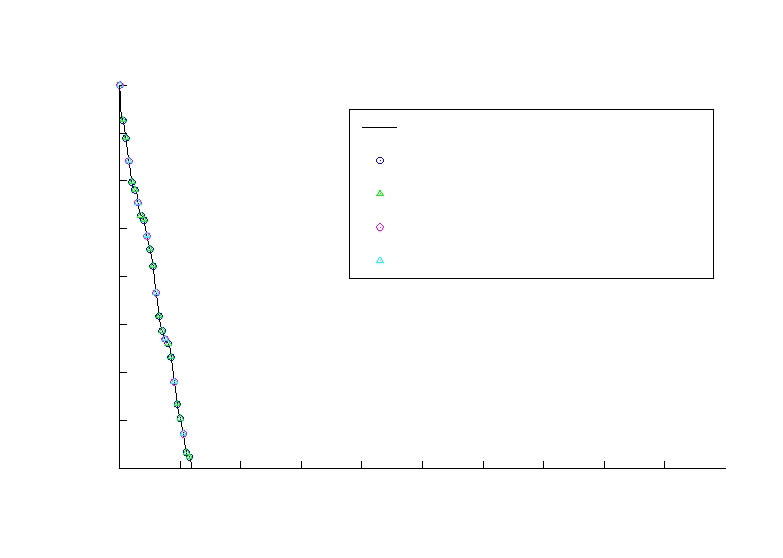
\includegraphics{watt1_ilu0}}%
    \gplfronttext
  \end{picture}%
\endgroup
}
	\caption{without basis vector scaling}
	\label{fig:watt1_ilu0}
\end{figure}
\begin{figure}
	\centering
	\resizebox{.9\textwidth}{!}{% GNUPLOT: LaTeX picture with Postscript
\begingroup
  \fontfamily{phv}%
  \selectfont
  \makeatletter
  \providecommand\color[2][]{%
    \GenericError{(gnuplot) \space\space\space\@spaces}{%
      Package color not loaded in conjunction with
      terminal option `colourtext'%
    }{See the gnuplot documentation for explanation.%
    }{Either use 'blacktext' in gnuplot or load the package
      color.sty in LaTeX.}%
    \renewcommand\color[2][]{}%
  }%
  \providecommand\includegraphics[2][]{%
    \GenericError{(gnuplot) \space\space\space\@spaces}{%
      Package graphicx or graphics not loaded%
    }{See the gnuplot documentation for explanation.%
    }{The gnuplot epslatex terminal needs graphicx.sty or graphics.sty.}%
    \renewcommand\includegraphics[2][]{}%
  }%
  \providecommand\rotatebox[2]{#2}%
  \@ifundefined{ifGPcolor}{%
    \newif\ifGPcolor
    \GPcolorfalse
  }{}%
  \@ifundefined{ifGPblacktext}{%
    \newif\ifGPblacktext
    \GPblacktexttrue
  }{}%
  % define a \g@addto@macro without @ in the name:
  \let\gplgaddtomacro\g@addto@macro
  % define empty templates for all commands taking text:
  \gdef\gplbacktext{}%
  \gdef\gplfronttext{}%
  \makeatother
  \ifGPblacktext
    % no textcolor at all
    \def\colorrgb#1{}%
    \def\colorgray#1{}%
  \else
    % gray or color?
    \ifGPcolor
      \def\colorrgb#1{\color[rgb]{#1}}%
      \def\colorgray#1{\color[gray]{#1}}%
      \expandafter\def\csname LTw\endcsname{\color{white}}%
      \expandafter\def\csname LTb\endcsname{\color{black}}%
      \expandafter\def\csname LTa\endcsname{\color{black}}%
      \expandafter\def\csname LT0\endcsname{\color[rgb]{1,0,0}}%
      \expandafter\def\csname LT1\endcsname{\color[rgb]{0,1,0}}%
      \expandafter\def\csname LT2\endcsname{\color[rgb]{0,0,1}}%
      \expandafter\def\csname LT3\endcsname{\color[rgb]{1,0,1}}%
      \expandafter\def\csname LT4\endcsname{\color[rgb]{0,1,1}}%
      \expandafter\def\csname LT5\endcsname{\color[rgb]{1,1,0}}%
      \expandafter\def\csname LT6\endcsname{\color[rgb]{0,0,0}}%
      \expandafter\def\csname LT7\endcsname{\color[rgb]{1,0.3,0}}%
      \expandafter\def\csname LT8\endcsname{\color[rgb]{0.5,0.5,0.5}}%
    \else
      % gray
      \def\colorrgb#1{\color{black}}%
      \def\colorgray#1{\color[gray]{#1}}%
      \expandafter\def\csname LTw\endcsname{\color{white}}%
      \expandafter\def\csname LTb\endcsname{\color{black}}%
      \expandafter\def\csname LTa\endcsname{\color{black}}%
      \expandafter\def\csname LT0\endcsname{\color{black}}%
      \expandafter\def\csname LT1\endcsname{\color{black}}%
      \expandafter\def\csname LT2\endcsname{\color{black}}%
      \expandafter\def\csname LT3\endcsname{\color{black}}%
      \expandafter\def\csname LT4\endcsname{\color{black}}%
      \expandafter\def\csname LT5\endcsname{\color{black}}%
      \expandafter\def\csname LT6\endcsname{\color{black}}%
      \expandafter\def\csname LT7\endcsname{\color{black}}%
      \expandafter\def\csname LT8\endcsname{\color{black}}%
    \fi
  \fi
    \setlength{\unitlength}{0.0500bp}%
    \ifx\gptboxheight\undefined%
      \newlength{\gptboxheight}%
      \newlength{\gptboxwidth}%
      \newsavebox{\gptboxtext}%
    \fi%
    \setlength{\fboxrule}{0.5pt}%
    \setlength{\fboxsep}{1pt}%
\begin{picture}(7200.00,5040.00)%
    \gplgaddtomacro\gplbacktext{%
      \csname LTb\endcsname%
      \put(726,704){\makebox(0,0)[r]{\strut{}\footnotesize -4}}%
      \put(726,1623){\makebox(0,0)[r]{\strut{}\footnotesize -3}}%
      \put(726,2542){\makebox(0,0)[r]{\strut{}\footnotesize -2}}%
      \put(726,3460){\makebox(0,0)[r]{\strut{}\footnotesize -1}}%
      \put(726,4379){\makebox(0,0)[r]{\strut{}\footnotesize 0}}%
      \put(1453,484){\makebox(0,0){\strut{}\footnotesize 100}}%
      \put(2047,484){\makebox(0,0){\strut{}\footnotesize 200}}%
      \put(2642,484){\makebox(0,0){\strut{}\footnotesize 300}}%
      \put(3236,484){\makebox(0,0){\strut{}\footnotesize 400}}%
      \put(3831,484){\makebox(0,0){\strut{}\footnotesize 500}}%
      \put(4425,484){\makebox(0,0){\strut{}\footnotesize 600}}%
      \put(5020,484){\makebox(0,0){\strut{}\footnotesize 700}}%
      \put(5614,484){\makebox(0,0){\strut{}\footnotesize 800}}%
      \put(6209,484){\makebox(0,0){\strut{}\footnotesize 900}}%
			\put(6803,484){\makebox(0,0){\strut{}\footnotesize 1000}}%
    }%
    \gplgaddtomacro\gplfronttext{%
      \csname LTb\endcsname%
      \put(352,2541){\rotatebox{-270}{\makebox(0,0){\strut{}\footnotesize Residual 2-norm, log scale}}}%
      \put(3830,154){\makebox(0,0){\strut{}\footnotesize Iteration count}}%
      \put(3830,4709){\makebox(0,0){\strut{}\shortstack{pwtk}}}%
      \csname LTb\endcsname%
      \put(2591,4161){\makebox(0,0)[l]{\strut{}\scriptsize GMRES(20)}}%
      \csname LTb\endcsname%
      \put(2591,3842){\makebox(0,0)[l]{\strut{}\begin{minipage}[l]{.95\textwidth} \scriptsize Monomial-GMRES(5,4) \newline \tiny min, max basis rcond \#: 3.47e-33, 2.51e-32\end{minipage}}}%
      \csname LTb\endcsname%
      \put(2591,3523){\makebox(0,0)[l]{\strut{}\begin{minipage}[l]{.95\textwidth} \scriptsize Newton-GMRES(5,4) \newline \tiny min, max basis rcond \#: 9.33e-32, 8.36e-30\end{minipage}}}%
      \csname LTb\endcsname%
      \put(2591,3204){\makebox(0,0)[l]{\strut{}\begin{minipage}[l]{.95\textwidth} \scriptsize Monomial-GMRES(10,2) \newline \tiny min, max basis rcond \#: 3.61e-72, 2.91e-71\end{minipage}}}%
      \csname LTb\endcsname%
      \put(2591,2885){\makebox(0,0)[l]{\strut{}\begin{minipage}[l]{.95\textwidth} \scriptsize Newton-GMRES(10,2) \newline \tiny min, max basis rcond \#: 5.92e-68, 5.99e-66\end{minipage}}}%
    }%
    \gplbacktext
    \put(0,0){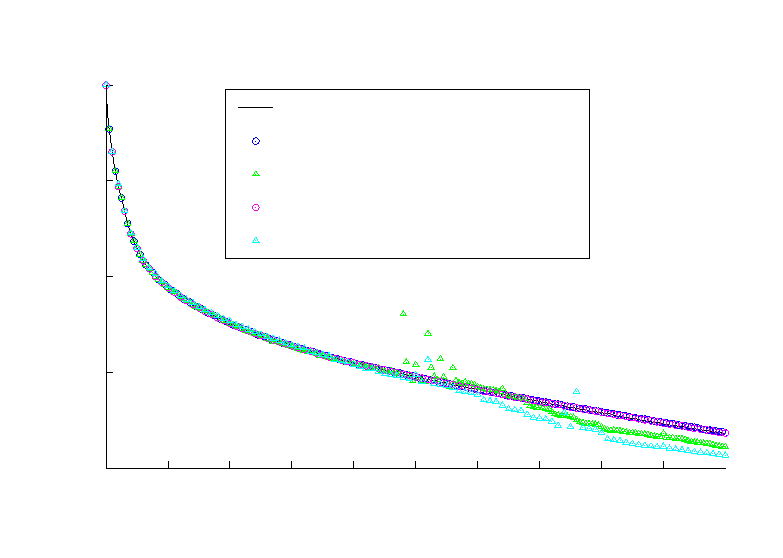
\includegraphics{pwtk_noscale}}%
    \gplfronttext
  \end{picture}%
\endgroup
}
	\caption{•••}
	\label{fig:pwtk_noscale}
\end{figure}
\begin{figure}
	\centering
	\resizebox{.9\textwidth}{!}{% GNUPLOT: LaTeX picture with Postscript
\begingroup
  \fontfamily{phv}%
  \selectfont
  \makeatletter
  \providecommand\color[2][]{%
    \GenericError{(gnuplot) \space\space\space\@spaces}{%
      Package color not loaded in conjunction with
      terminal option `colourtext'%
    }{See the gnuplot documentation for explanation.%
    }{Either use 'blacktext' in gnuplot or load the package
      color.sty in LaTeX.}%
    \renewcommand\color[2][]{}%
  }%
  \providecommand\includegraphics[2][]{%
    \GenericError{(gnuplot) \space\space\space\@spaces}{%
      Package graphicx or graphics not loaded%
    }{See the gnuplot documentation for explanation.%
    }{The gnuplot epslatex terminal needs graphicx.sty or graphics.sty.}%
    \renewcommand\includegraphics[2][]{}%
  }%
  \providecommand\rotatebox[2]{#2}%
  \@ifundefined{ifGPcolor}{%
    \newif\ifGPcolor
    \GPcolorfalse
  }{}%
  \@ifundefined{ifGPblacktext}{%
    \newif\ifGPblacktext
    \GPblacktexttrue
  }{}%
  % define a \g@addto@macro without @ in the name:
  \let\gplgaddtomacro\g@addto@macro
  % define empty templates for all commands taking text:
  \gdef\gplbacktext{}%
  \gdef\gplfronttext{}%
  \makeatother
  \ifGPblacktext
    % no textcolor at all
    \def\colorrgb#1{}%
    \def\colorgray#1{}%
  \else
    % gray or color?
    \ifGPcolor
      \def\colorrgb#1{\color[rgb]{#1}}%
      \def\colorgray#1{\color[gray]{#1}}%
      \expandafter\def\csname LTw\endcsname{\color{white}}%
      \expandafter\def\csname LTb\endcsname{\color{black}}%
      \expandafter\def\csname LTa\endcsname{\color{black}}%
      \expandafter\def\csname LT0\endcsname{\color[rgb]{1,0,0}}%
      \expandafter\def\csname LT1\endcsname{\color[rgb]{0,1,0}}%
      \expandafter\def\csname LT2\endcsname{\color[rgb]{0,0,1}}%
      \expandafter\def\csname LT3\endcsname{\color[rgb]{1,0,1}}%
      \expandafter\def\csname LT4\endcsname{\color[rgb]{0,1,1}}%
      \expandafter\def\csname LT5\endcsname{\color[rgb]{1,1,0}}%
      \expandafter\def\csname LT6\endcsname{\color[rgb]{0,0,0}}%
      \expandafter\def\csname LT7\endcsname{\color[rgb]{1,0.3,0}}%
      \expandafter\def\csname LT8\endcsname{\color[rgb]{0.5,0.5,0.5}}%
    \else
      % gray
      \def\colorrgb#1{\color{black}}%
      \def\colorgray#1{\color[gray]{#1}}%
      \expandafter\def\csname LTw\endcsname{\color{white}}%
      \expandafter\def\csname LTb\endcsname{\color{black}}%
      \expandafter\def\csname LTa\endcsname{\color{black}}%
      \expandafter\def\csname LT0\endcsname{\color{black}}%
      \expandafter\def\csname LT1\endcsname{\color{black}}%
      \expandafter\def\csname LT2\endcsname{\color{black}}%
      \expandafter\def\csname LT3\endcsname{\color{black}}%
      \expandafter\def\csname LT4\endcsname{\color{black}}%
      \expandafter\def\csname LT5\endcsname{\color{black}}%
      \expandafter\def\csname LT6\endcsname{\color{black}}%
      \expandafter\def\csname LT7\endcsname{\color{black}}%
      \expandafter\def\csname LT8\endcsname{\color{black}}%
    \fi
  \fi
    \setlength{\unitlength}{0.0500bp}%
    \ifx\gptboxheight\undefined%
      \newlength{\gptboxheight}%
      \newlength{\gptboxwidth}%
      \newsavebox{\gptboxtext}%
    \fi%
    \setlength{\fboxrule}{0.5pt}%
    \setlength{\fboxsep}{1pt}%
\begin{picture}(7200.00,5040.00)%
    \gplgaddtomacro\gplbacktext{%
      \csname LTb\endcsname%
      \put(726,704){\makebox(0,0)[r]{\strut{}\footnotesize -4}}%
      \put(726,1623){\makebox(0,0)[r]{\strut{}\footnotesize -3}}%
      \put(726,2542){\makebox(0,0)[r]{\strut{}\footnotesize -2}}%
      \put(726,3460){\makebox(0,0)[r]{\strut{}\footnotesize -1}}%
      \put(726,4379){\makebox(0,0)[r]{\strut{}\footnotesize 0}}%
      \put(1453,484){\makebox(0,0){\strut{}\footnotesize 100}}%
      \put(2047,484){\makebox(0,0){\strut{}\footnotesize 200}}%
      \put(2642,484){\makebox(0,0){\strut{}\footnotesize 300}}%
      \put(3236,484){\makebox(0,0){\strut{}\footnotesize 400}}%
      \put(3831,484){\makebox(0,0){\strut{}\footnotesize 500}}%
      \put(4425,484){\makebox(0,0){\strut{}\footnotesize 600}}%
      \put(5020,484){\makebox(0,0){\strut{}\footnotesize 700}}%
      \put(5614,484){\makebox(0,0){\strut{}\footnotesize 800}}%
      \put(6209,484){\makebox(0,0){\strut{}\footnotesize 900}}%
			\put(6803,484){\makebox(0,0){\strut{}\footnotesize 1000}}%
    }%
    \gplgaddtomacro\gplfronttext{%
      \csname LTb\endcsname%
      \put(352,2541){\rotatebox{-270}{\makebox(0,0){\strut{}\footnotesize Residual 2-norm, log scale}}}%
      \put(3830,154){\makebox(0,0){\strut{}\footnotesize Iteration count}}%
      \put(3830,4709){\makebox(0,0){\strut{}\shortstack{pwtk}}}%
      \csname LTb\endcsname%
      \put(2591,4161){\makebox(0,0)[l]{\strut{}\scriptsize GMRES(20)}}%
      \csname LTb\endcsname%
      \put(2591,3842){\makebox(0,0)[l]{\strut{}\begin{minipage}[l]{.95\textwidth} \scriptsize Monomial-GMRES(5,4) \newline \tiny min, max basis rcond \#: 3.08e-11, 3.13e-10\end{minipage}}}%
      \csname LTb\endcsname%
      \put(2591,3523){\makebox(0,0)[l]{\strut{}\begin{minipage}[l]{.95\textwidth} \scriptsize Newton-GMRES(5,4) \newline \tiny min, max basis rcond \#: 7.48e-16, 2.46e-08\end{minipage}}}%
      \csname LTb\endcsname%
      \put(2591,3204){\makebox(0,0)[l]{\strut{}\begin{minipage}[l]{.95\textwidth} \scriptsize Monomial-GMRES(10,2) \newline \tiny min, max basis rcond \#: 3.27e-14, 3.84e-13\end{minipage}}}%
      \csname LTb\endcsname%
      \put(2591,2885){\makebox(0,0)[l]{\strut{}\begin{minipage}[l]{.95\textwidth} \scriptsize Newton-GMRES(10,2) \newline \tiny min, max basis rcond \#: 1.38e-23, 6.42e-23\end{minipage}}}%
    }%
    \gplbacktext
    \put(0,0){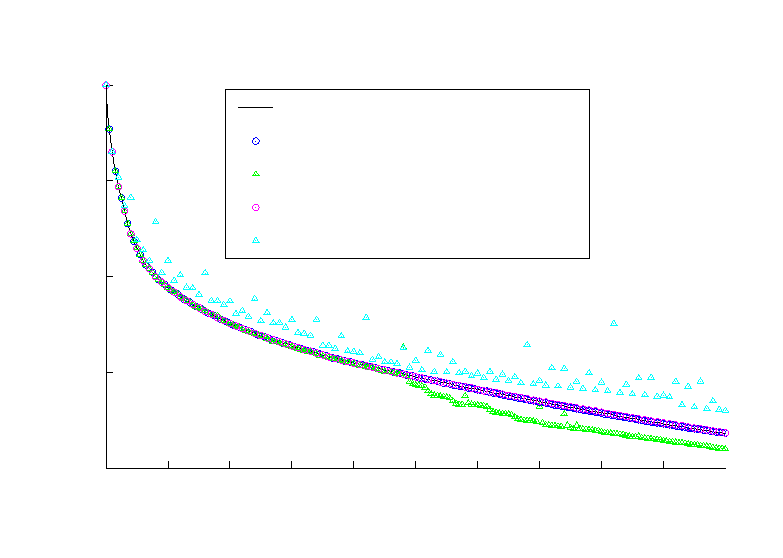
\includegraphics{pwtk_scale}}%
    \gplfronttext
  \end{picture}%
\endgroup
}
	\caption{•••}
	\label{fig:pwtk_scale}
\end{figure}
\begin{figure}
	\centering
	\resizebox{.9\textwidth}{!}{% GNUPLOT: LaTeX picture with Postscript
\begingroup
  \fontfamily{phv}%
  \selectfont
  \makeatletter
  \providecommand\color[2][]{%
    \GenericError{(gnuplot) \space\space\space\@spaces}{%
      Package color not loaded in conjunction with
      terminal option `colourtext'%
    }{See the gnuplot documentation for explanation.%
    }{Either use 'blacktext' in gnuplot or load the package
      color.sty in LaTeX.}%
    \renewcommand\color[2][]{}%
  }%
  \providecommand\includegraphics[2][]{%
    \GenericError{(gnuplot) \space\space\space\@spaces}{%
      Package graphicx or graphics not loaded%
    }{See the gnuplot documentation for explanation.%
    }{The gnuplot epslatex terminal needs graphicx.sty or graphics.sty.}%
    \renewcommand\includegraphics[2][]{}%
  }%
  \providecommand\rotatebox[2]{#2}%
  \@ifundefined{ifGPcolor}{%
    \newif\ifGPcolor
    \GPcolorfalse
  }{}%
  \@ifundefined{ifGPblacktext}{%
    \newif\ifGPblacktext
    \GPblacktexttrue
  }{}%
  % define a \g@addto@macro without @ in the name:
  \let\gplgaddtomacro\g@addto@macro
  % define empty templates for all commands taking text:
  \gdef\gplbacktext{}%
  \gdef\gplfronttext{}%
  \makeatother
  \ifGPblacktext
    % no textcolor at all
    \def\colorrgb#1{}%
    \def\colorgray#1{}%
  \else
    % gray or color?
    \ifGPcolor
      \def\colorrgb#1{\color[rgb]{#1}}%
      \def\colorgray#1{\color[gray]{#1}}%
      \expandafter\def\csname LTw\endcsname{\color{white}}%
      \expandafter\def\csname LTb\endcsname{\color{black}}%
      \expandafter\def\csname LTa\endcsname{\color{black}}%
      \expandafter\def\csname LT0\endcsname{\color[rgb]{1,0,0}}%
      \expandafter\def\csname LT1\endcsname{\color[rgb]{0,1,0}}%
      \expandafter\def\csname LT2\endcsname{\color[rgb]{0,0,1}}%
      \expandafter\def\csname LT3\endcsname{\color[rgb]{1,0,1}}%
      \expandafter\def\csname LT4\endcsname{\color[rgb]{0,1,1}}%
      \expandafter\def\csname LT5\endcsname{\color[rgb]{1,1,0}}%
      \expandafter\def\csname LT6\endcsname{\color[rgb]{0,0,0}}%
      \expandafter\def\csname LT7\endcsname{\color[rgb]{1,0.3,0}}%
      \expandafter\def\csname LT8\endcsname{\color[rgb]{0.5,0.5,0.5}}%
    \else
      % gray
      \def\colorrgb#1{\color{black}}%
      \def\colorgray#1{\color[gray]{#1}}%
      \expandafter\def\csname LTw\endcsname{\color{white}}%
      \expandafter\def\csname LTb\endcsname{\color{black}}%
      \expandafter\def\csname LTa\endcsname{\color{black}}%
      \expandafter\def\csname LT0\endcsname{\color{black}}%
      \expandafter\def\csname LT1\endcsname{\color{black}}%
      \expandafter\def\csname LT2\endcsname{\color{black}}%
      \expandafter\def\csname LT3\endcsname{\color{black}}%
      \expandafter\def\csname LT4\endcsname{\color{black}}%
      \expandafter\def\csname LT5\endcsname{\color{black}}%
      \expandafter\def\csname LT6\endcsname{\color{black}}%
      \expandafter\def\csname LT7\endcsname{\color{black}}%
      \expandafter\def\csname LT8\endcsname{\color{black}}%
    \fi
  \fi
    \setlength{\unitlength}{0.0500bp}%
    \ifx\gptboxheight\undefined%
      \newlength{\gptboxheight}%
      \newlength{\gptboxwidth}%
      \newsavebox{\gptboxtext}%
    \fi%
    \setlength{\fboxrule}{0.5pt}%
    \setlength{\fboxsep}{1pt}%
\begin{picture}(7200.00,5040.00)%
    \gplgaddtomacro\gplbacktext{%
      \csname LTb\endcsname%
      \put(858,4195){\makebox(0,0)[r]{\strut{}\footnotesize -16}}%
      \put(858,4207){\makebox(0,0)[r]{\strut{}\footnotesize -15}}%
      \put(858,4218){\makebox(0,0)[r]{\strut{}\footnotesize -14}}%
      \put(858,4230){\makebox(0,0)[r]{\strut{}\footnotesize -13}}%
      \put(858,4241){\makebox(0,0)[r]{\strut{}\footnotesize -12}}%
      \put(858,4253){\makebox(0,0)[r]{\strut{}\footnotesize -11}}%
      \put(858,4264){\makebox(0,0)[r]{\strut{}\footnotesize -10}}%
      \put(858,4276){\makebox(0,0)[r]{\strut{}\footnotesize -9}}%
      \put(858,4287){\makebox(0,0)[r]{\strut{}\footnotesize -8}}%
      \put(858,4299){\makebox(0,0)[r]{\strut{}\footnotesize -7}}%
      \put(858,4310){\makebox(0,0)[r]{\strut{}\footnotesize -6}}%
      \put(858,4322){\makebox(0,0)[r]{\strut{}\footnotesize -5}}%
      \put(858,4333){\makebox(0,0)[r]{\strut{}\footnotesize -4}}%
      \put(858,4345){\makebox(0,0)[r]{\strut{}\footnotesize -3}}%
      \put(858,4356){\makebox(0,0)[r]{\strut{}\footnotesize -2}}%
      \put(858,4368){\makebox(0,0)[r]{\strut{}\footnotesize -1}}%
      \put(858,4379){\makebox(0,0)[r]{\strut{}\footnotesize 0}}%
      \put(1898,484){\makebox(0,0){\strut{}\footnotesize 5}}%
      \put(2807,484){\makebox(0,0){\strut{}\footnotesize 10}}%
      \put(3715,484){\makebox(0,0){\strut{}\footnotesize 15}}%
      \put(4623,484){\makebox(0,0){\strut{}\footnotesize 20}}%
      \put(5531,484){\makebox(0,0){\strut{}\footnotesize 25}}%
      \put(6440,484){\makebox(0,0){\strut{}\footnotesize 30}}%
    }%
    \gplgaddtomacro\gplfronttext{%
      \csname LTb\endcsname%
      \put(352,2541){\rotatebox{-270}{\makebox(0,0){\strut{}\footnotesize Residual 2-norm, log scale}}}%
      \put(3896,154){\makebox(0,0){\strut{}\footnotesize Iteration count}}%
      \put(3896,4709){\makebox(0,0){\strut{}\shortstack{bmw}}}%
      \csname LTb\endcsname%
      \put(4295,2217){\makebox(0,0)[l]{\strut{}\scriptsize GMRES(20)}}%
      \csname LTb\endcsname%
      \put(4295,1898){\makebox(0,0)[l]{\strut{}\begin{minipage}[l]{.95\textwidth} \scriptsize Monomial-GMRES(5,4) \newline \tiny min, max basis rcond \#: 1.87e-01, 1.87e-01\end{minipage}}}%
      \csname LTb\endcsname%
      \put(4295,1579){\makebox(0,0)[l]{\strut{}\begin{minipage}[l]{.95\textwidth} \scriptsize Newton-GMRES(5,4) \newline \tiny min, max basis rcond \#: 1.25e-16, 1.25e-16\end{minipage}}}%
      \csname LTb\endcsname%
      \put(4295,1260){\makebox(0,0)[l]{\strut{}\begin{minipage}[l]{.95\textwidth} \scriptsize Monomial-GMRES(10,2) \newline \tiny min, max basis rcond \#: 1.40e-01, 1.40e-01\end{minipage}}}%
      \csname LTb\endcsname%
      \put(4295,941){\makebox(0,0)[l]{\strut{}\begin{minipage}[l]{.95\textwidth} \scriptsize Newton-GMRES(10,2) \newline \tiny min, max basis rcond \#: 1.69e-17, 1.69e-17\end{minipage}}}%
    }%
    \gplbacktext
    \put(0,0){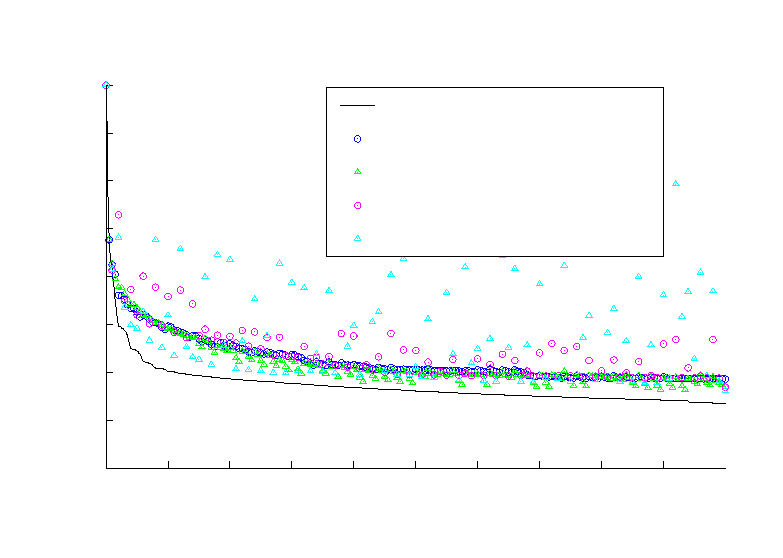
\includegraphics{bmw7st1}}%
    \gplfronttext
  \end{picture}%
\endgroup
}
	\caption{•••}
	\label{fig:bmw7st1}
\end{figure}
\begin{figure}
	\centering
	\resizebox{.9\textwidth}{!}{% GNUPLOT: LaTeX picture with Postscript
\begingroup
  \fontfamily{phv}%
  \selectfont
  \makeatletter
  \providecommand\color[2][]{%
    \GenericError{(gnuplot) \space\space\space\@spaces}{%
      Package color not loaded in conjunction with
      terminal option `colourtext'%
    }{See the gnuplot documentation for explanation.%
    }{Either use 'blacktext' in gnuplot or load the package
      color.sty in LaTeX.}%
    \renewcommand\color[2][]{}%
  }%
  \providecommand\includegraphics[2][]{%
    \GenericError{(gnuplot) \space\space\space\@spaces}{%
      Package graphicx or graphics not loaded%
    }{See the gnuplot documentation for explanation.%
    }{The gnuplot epslatex terminal needs graphicx.sty or graphics.sty.}%
    \renewcommand\includegraphics[2][]{}%
  }%
  \providecommand\rotatebox[2]{#2}%
  \@ifundefined{ifGPcolor}{%
    \newif\ifGPcolor
    \GPcolorfalse
  }{}%
  \@ifundefined{ifGPblacktext}{%
    \newif\ifGPblacktext
    \GPblacktexttrue
  }{}%
  % define a \g@addto@macro without @ in the name:
  \let\gplgaddtomacro\g@addto@macro
  % define empty templates for all commands taking text:
  \gdef\gplbacktext{}%
  \gdef\gplfronttext{}%
  \makeatother
  \ifGPblacktext
    % no textcolor at all
    \def\colorrgb#1{}%
    \def\colorgray#1{}%
  \else
    % gray or color?
    \ifGPcolor
      \def\colorrgb#1{\color[rgb]{#1}}%
      \def\colorgray#1{\color[gray]{#1}}%
      \expandafter\def\csname LTw\endcsname{\color{white}}%
      \expandafter\def\csname LTb\endcsname{\color{black}}%
      \expandafter\def\csname LTa\endcsname{\color{black}}%
      \expandafter\def\csname LT0\endcsname{\color[rgb]{1,0,0}}%
      \expandafter\def\csname LT1\endcsname{\color[rgb]{0,1,0}}%
      \expandafter\def\csname LT2\endcsname{\color[rgb]{0,0,1}}%
      \expandafter\def\csname LT3\endcsname{\color[rgb]{1,0,1}}%
      \expandafter\def\csname LT4\endcsname{\color[rgb]{0,1,1}}%
      \expandafter\def\csname LT5\endcsname{\color[rgb]{1,1,0}}%
      \expandafter\def\csname LT6\endcsname{\color[rgb]{0,0,0}}%
      \expandafter\def\csname LT7\endcsname{\color[rgb]{1,0.3,0}}%
      \expandafter\def\csname LT8\endcsname{\color[rgb]{0.5,0.5,0.5}}%
    \else
      % gray
      \def\colorrgb#1{\color{black}}%
      \def\colorgray#1{\color[gray]{#1}}%
      \expandafter\def\csname LTw\endcsname{\color{white}}%
      \expandafter\def\csname LTb\endcsname{\color{black}}%
      \expandafter\def\csname LTa\endcsname{\color{black}}%
      \expandafter\def\csname LT0\endcsname{\color{black}}%
      \expandafter\def\csname LT1\endcsname{\color{black}}%
      \expandafter\def\csname LT2\endcsname{\color{black}}%
      \expandafter\def\csname LT3\endcsname{\color{black}}%
      \expandafter\def\csname LT4\endcsname{\color{black}}%
      \expandafter\def\csname LT5\endcsname{\color{black}}%
      \expandafter\def\csname LT6\endcsname{\color{black}}%
      \expandafter\def\csname LT7\endcsname{\color{black}}%
      \expandafter\def\csname LT8\endcsname{\color{black}}%
    \fi
  \fi
    \setlength{\unitlength}{0.0500bp}%
    \ifx\gptboxheight\undefined%
      \newlength{\gptboxheight}%
      \newlength{\gptboxwidth}%
      \newsavebox{\gptboxtext}%
    \fi%
    \setlength{\fboxrule}{0.5pt}%
    \setlength{\fboxsep}{1pt}%
\begin{picture}(7200.00,5040.00)%
    \gplgaddtomacro\gplbacktext{%
      \csname LTb\endcsname%
      \put(726,704){\makebox(0,0)[r]{\strut{}\footnotesize -8}}%
      \put(726,1163){\makebox(0,0)[r]{\strut{}\footnotesize -7}}%
      \put(726,1623){\makebox(0,0)[r]{\strut{}\footnotesize -6}}%
      \put(726,2082){\makebox(0,0)[r]{\strut{}\footnotesize -5}}%
      \put(726,2542){\makebox(0,0)[r]{\strut{}\footnotesize -4}}%
      \put(726,3001){\makebox(0,0)[r]{\strut{}\footnotesize -3}}%
      \put(726,3460){\makebox(0,0)[r]{\strut{}\footnotesize -2}}%
      \put(726,3920){\makebox(0,0)[r]{\strut{}\footnotesize -1}}%
      \put(726,4379){\makebox(0,0)[r]{\strut{}\footnotesize 0}}%
      \put(1453,484){\makebox(0,0){\strut{}\footnotesize 100}}%
      \put(2047,484){\makebox(0,0){\strut{}\footnotesize 200}}%
      \put(2642,484){\makebox(0,0){\strut{}\footnotesize 300}}%
      \put(3236,484){\makebox(0,0){\strut{}\footnotesize 400}}%
      \put(3831,484){\makebox(0,0){\strut{}\footnotesize 500}}%
      \put(4425,484){\makebox(0,0){\strut{}\footnotesize 600}}%
      \put(5020,484){\makebox(0,0){\strut{}\footnotesize 700}}%
      \put(5614,484){\makebox(0,0){\strut{}\footnotesize 800}}%
      \put(6209,484){\makebox(0,0){\strut{}\footnotesize 900}}%
    }%
    \gplgaddtomacro\gplfronttext{%
      \csname LTb\endcsname%
      \put(352,2541){\rotatebox{-270}{\makebox(0,0){\strut{}\footnotesize Residual 2-norm, log scale}}}%
      \put(3830,154){\makebox(0,0){\strut{}\footnotesize Iteration count}}%
      \put(3830,4709){\makebox(0,0){\strut{}\shortstack{bmw}}}%
      \csname LTb\endcsname%
      \put(3833,4182){\makebox(0,0)[l]{\strut{}\scriptsize GMRES(20)}}%
      \csname LTb\endcsname%
      \put(3833,3863){\makebox(0,0)[l]{\strut{}\begin{minipage}[l]{.95\textwidth} \scriptsize Monomial-GMRES(5,4) \newline \tiny min, max basis rcond \#: 1.51e-12, 8.52e-06\end{minipage}}}%
      \csname LTb\endcsname%
      \put(3833,3544){\makebox(0,0)[l]{\strut{}\begin{minipage}[l]{.95\textwidth} \scriptsize Newton-GMRES(5,4) \newline \tiny min, max basis rcond \#: 1.11e-12, 8.18e-04\end{minipage}}}%
      \csname LTb\endcsname%
      \put(3833,3225){\makebox(0,0)[l]{\strut{}\begin{minipage}[l]{.95\textwidth} \scriptsize Monomial-GMRES(10,2) \newline \tiny min, max basis rcond \#: 2.02e-18, 4.03e-15\end{minipage}}}%
      \csname LTb\endcsname%
      \put(3833,2906){\makebox(0,0)[l]{\strut{}\begin{minipage}[l]{.95\textwidth} \scriptsize Newton-GMRES(10,2) \newline \tiny min, max basis rcond \#: 3.54e-17, 4.84e-15\end{minipage}}}%
    }%
    \gplbacktext
    \put(0,0){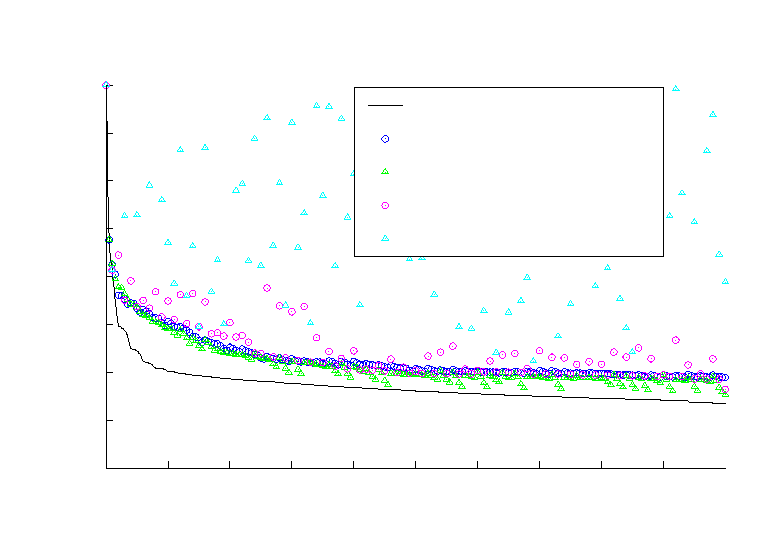
\includegraphics{bmw7st1_scale}}%
    \gplfronttext
  \end{picture}%
\endgroup
}
	\caption{•••}
	\label{fig:bmw7st1_scale}
\end{figure}
\begin{figure}
	\centering
	\resizebox{.9\textwidth}{!}{% GNUPLOT: LaTeX picture with Postscript
\begingroup
  \fontfamily{phv}%
  \selectfont
  \makeatletter
  \providecommand\color[2][]{%
    \GenericError{(gnuplot) \space\space\space\@spaces}{%
      Package color not loaded in conjunction with
      terminal option `colourtext'%
    }{See the gnuplot documentation for explanation.%
    }{Either use 'blacktext' in gnuplot or load the package
      color.sty in LaTeX.}%
    \renewcommand\color[2][]{}%
  }%
  \providecommand\includegraphics[2][]{%
    \GenericError{(gnuplot) \space\space\space\@spaces}{%
      Package graphicx or graphics not loaded%
    }{See the gnuplot documentation for explanation.%
    }{The gnuplot epslatex terminal needs graphicx.sty or graphics.sty.}%
    \renewcommand\includegraphics[2][]{}%
  }%
  \providecommand\rotatebox[2]{#2}%
  \@ifundefined{ifGPcolor}{%
    \newif\ifGPcolor
    \GPcolorfalse
  }{}%
  \@ifundefined{ifGPblacktext}{%
    \newif\ifGPblacktext
    \GPblacktexttrue
  }{}%
  % define a \g@addto@macro without @ in the name:
  \let\gplgaddtomacro\g@addto@macro
  % define empty templates for all commands taking text:
  \gdef\gplbacktext{}%
  \gdef\gplfronttext{}%
  \makeatother
  \ifGPblacktext
    % no textcolor at all
    \def\colorrgb#1{}%
    \def\colorgray#1{}%
  \else
    % gray or color?
    \ifGPcolor
      \def\colorrgb#1{\color[rgb]{#1}}%
      \def\colorgray#1{\color[gray]{#1}}%
      \expandafter\def\csname LTw\endcsname{\color{white}}%
      \expandafter\def\csname LTb\endcsname{\color{black}}%
      \expandafter\def\csname LTa\endcsname{\color{black}}%
      \expandafter\def\csname LT0\endcsname{\color[rgb]{1,0,0}}%
      \expandafter\def\csname LT1\endcsname{\color[rgb]{0,1,0}}%
      \expandafter\def\csname LT2\endcsname{\color[rgb]{0,0,1}}%
      \expandafter\def\csname LT3\endcsname{\color[rgb]{1,0,1}}%
      \expandafter\def\csname LT4\endcsname{\color[rgb]{0,1,1}}%
      \expandafter\def\csname LT5\endcsname{\color[rgb]{1,1,0}}%
      \expandafter\def\csname LT6\endcsname{\color[rgb]{0,0,0}}%
      \expandafter\def\csname LT7\endcsname{\color[rgb]{1,0.3,0}}%
      \expandafter\def\csname LT8\endcsname{\color[rgb]{0.5,0.5,0.5}}%
    \else
      % gray
      \def\colorrgb#1{\color{black}}%
      \def\colorgray#1{\color[gray]{#1}}%
      \expandafter\def\csname LTw\endcsname{\color{white}}%
      \expandafter\def\csname LTb\endcsname{\color{black}}%
      \expandafter\def\csname LTa\endcsname{\color{black}}%
      \expandafter\def\csname LT0\endcsname{\color{black}}%
      \expandafter\def\csname LT1\endcsname{\color{black}}%
      \expandafter\def\csname LT2\endcsname{\color{black}}%
      \expandafter\def\csname LT3\endcsname{\color{black}}%
      \expandafter\def\csname LT4\endcsname{\color{black}}%
      \expandafter\def\csname LT5\endcsname{\color{black}}%
      \expandafter\def\csname LT6\endcsname{\color{black}}%
      \expandafter\def\csname LT7\endcsname{\color{black}}%
      \expandafter\def\csname LT8\endcsname{\color{black}}%
    \fi
  \fi
    \setlength{\unitlength}{0.0500bp}%
    \ifx\gptboxheight\undefined%
      \newlength{\gptboxheight}%
      \newlength{\gptboxwidth}%
      \newsavebox{\gptboxtext}%
    \fi%
    \setlength{\fboxrule}{0.5pt}%
    \setlength{\fboxsep}{1pt}%
\begin{picture}(7200.00,5040.00)%
    \gplgaddtomacro\gplbacktext{%
      \csname LTb\endcsname%
      \put(726,704){\makebox(0,0)[r]{\strut{}\footnotesize -6}}%
      \put(726,1316){\makebox(0,0)[r]{\strut{}\footnotesize -5}}%
      \put(726,1929){\makebox(0,0)[r]{\strut{}\footnotesize -4}}%
      \put(726,2542){\makebox(0,0)[r]{\strut{}\footnotesize -3}}%
      \put(726,3154){\makebox(0,0)[r]{\strut{}\footnotesize -2}}%
      \put(726,3767){\makebox(0,0)[r]{\strut{}\footnotesize -1}}%
      \put(726,4379){\makebox(0,0)[r]{\strut{}\footnotesize 0}}%
      \put(1453,484){\makebox(0,0){\strut{}\footnotesize 100}}%
      \put(2047,484){\makebox(0,0){\strut{}\footnotesize 200}}%
      \put(2642,484){\makebox(0,0){\strut{}\footnotesize 300}}%
      \put(3236,484){\makebox(0,0){\strut{}\footnotesize 400}}%
      \put(3831,484){\makebox(0,0){\strut{}\footnotesize 500}}%
      \put(4425,484){\makebox(0,0){\strut{}\footnotesize 600}}%
      \put(5020,484){\makebox(0,0){\strut{}\footnotesize 700}}%
      \put(5614,484){\makebox(0,0){\strut{}\footnotesize 800}}%
      \put(6209,484){\makebox(0,0){\strut{}\footnotesize 900}}%
			\put(6803,484){\makebox(0,0){\strut{}\footnotesize 1000}}%
    }%
    \gplgaddtomacro\gplfronttext{%
      \csname LTb\endcsname%
      \put(352,2541){\rotatebox{-270}{\makebox(0,0){\strut{}\footnotesize Residual 2-norm, log scale}}}%
      \put(3830,154){\makebox(0,0){\strut{}\footnotesize Iteration count}}%
      \put(3830,4709){\makebox(0,0){\strut{}\shortstack{Xenon2}}}%
      \csname LTb\endcsname%
      \put(2380,3775){\makebox(0,0)[l]{\strut{}\scriptsize GMRES(20)}}%
      \csname LTb\endcsname%
      \put(2380,3456){\makebox(0,0)[l]{\strut{}\begin{minipage}[l]{.95\textwidth} \scriptsize Monomial-GMRES(5,4) \newline \tiny min, max basis rcond \#: 2.43e-117, 3.02e-117\end{minipage}}}%
      \csname LTb\endcsname%
      \put(2380,3137){\makebox(0,0)[l]{\strut{}\begin{minipage}[l]{.95\textwidth} \scriptsize Newton-GMRES(5,4) \newline \tiny min, max basis rcond \#: 5.37e-114, 1.59e-113\end{minipage}}}%
      \csname LTb\endcsname%
      \put(2380,2818){\makebox(0,0)[l]{\strut{}\begin{minipage}[l]{.95\textwidth} \scriptsize Monomial-GMRES(10,2) \newline \tiny min, max basis rcond \#: 1.17e-261, 1.40e-261\end{minipage}}}%
      \csname LTb\endcsname%
      \put(2380,2499){\makebox(0,0)[l]{\strut{}\begin{minipage}[l]{.95\textwidth} \scriptsize Newton-GMRES(10,2) \newline \tiny min, max basis rcond \#: 5.97e-255, 2.80e-254\end{minipage}}}%
    }%
    \gplbacktext
    \put(0,0){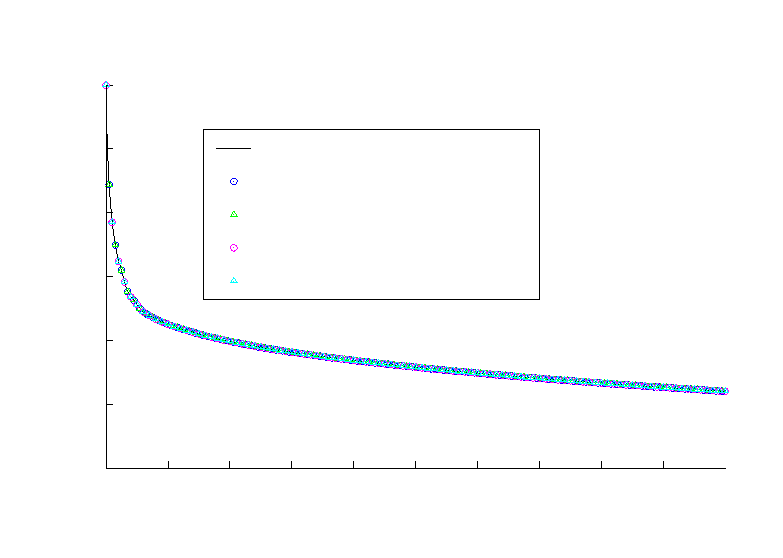
\includegraphics{xenon2}}%
    \gplfronttext
  \end{picture}%
\endgroup
}
	\caption{•••}
	\label{fig:xenon2}
\end{figure}
\begin{figure}
	\centering
	\resizebox{.9\textwidth}{!}{% GNUPLOT: LaTeX picture with Postscript
\begingroup
  \fontfamily{phv}%
  \selectfont
  \makeatletter
  \providecommand\color[2][]{%
    \GenericError{(gnuplot) \space\space\space\@spaces}{%
      Package color not loaded in conjunction with
      terminal option `colourtext'%
    }{See the gnuplot documentation for explanation.%
    }{Either use 'blacktext' in gnuplot or load the package
      color.sty in LaTeX.}%
    \renewcommand\color[2][]{}%
  }%
  \providecommand\includegraphics[2][]{%
    \GenericError{(gnuplot) \space\space\space\@spaces}{%
      Package graphicx or graphics not loaded%
    }{See the gnuplot documentation for explanation.%
    }{The gnuplot epslatex terminal needs graphicx.sty or graphics.sty.}%
    \renewcommand\includegraphics[2][]{}%
  }%
  \providecommand\rotatebox[2]{#2}%
  \@ifundefined{ifGPcolor}{%
    \newif\ifGPcolor
    \GPcolorfalse
  }{}%
  \@ifundefined{ifGPblacktext}{%
    \newif\ifGPblacktext
    \GPblacktexttrue
  }{}%
  % define a \g@addto@macro without @ in the name:
  \let\gplgaddtomacro\g@addto@macro
  % define empty templates for all commands taking text:
  \gdef\gplbacktext{}%
  \gdef\gplfronttext{}%
  \makeatother
  \ifGPblacktext
    % no textcolor at all
    \def\colorrgb#1{}%
    \def\colorgray#1{}%
  \else
    % gray or color?
    \ifGPcolor
      \def\colorrgb#1{\color[rgb]{#1}}%
      \def\colorgray#1{\color[gray]{#1}}%
      \expandafter\def\csname LTw\endcsname{\color{white}}%
      \expandafter\def\csname LTb\endcsname{\color{black}}%
      \expandafter\def\csname LTa\endcsname{\color{black}}%
      \expandafter\def\csname LT0\endcsname{\color[rgb]{1,0,0}}%
      \expandafter\def\csname LT1\endcsname{\color[rgb]{0,1,0}}%
      \expandafter\def\csname LT2\endcsname{\color[rgb]{0,0,1}}%
      \expandafter\def\csname LT3\endcsname{\color[rgb]{1,0,1}}%
      \expandafter\def\csname LT4\endcsname{\color[rgb]{0,1,1}}%
      \expandafter\def\csname LT5\endcsname{\color[rgb]{1,1,0}}%
      \expandafter\def\csname LT6\endcsname{\color[rgb]{0,0,0}}%
      \expandafter\def\csname LT7\endcsname{\color[rgb]{1,0.3,0}}%
      \expandafter\def\csname LT8\endcsname{\color[rgb]{0.5,0.5,0.5}}%
    \else
      % gray
      \def\colorrgb#1{\color{black}}%
      \def\colorgray#1{\color[gray]{#1}}%
      \expandafter\def\csname LTw\endcsname{\color{white}}%
      \expandafter\def\csname LTb\endcsname{\color{black}}%
      \expandafter\def\csname LTa\endcsname{\color{black}}%
      \expandafter\def\csname LT0\endcsname{\color{black}}%
      \expandafter\def\csname LT1\endcsname{\color{black}}%
      \expandafter\def\csname LT2\endcsname{\color{black}}%
      \expandafter\def\csname LT3\endcsname{\color{black}}%
      \expandafter\def\csname LT4\endcsname{\color{black}}%
      \expandafter\def\csname LT5\endcsname{\color{black}}%
      \expandafter\def\csname LT6\endcsname{\color{black}}%
      \expandafter\def\csname LT7\endcsname{\color{black}}%
      \expandafter\def\csname LT8\endcsname{\color{black}}%
    \fi
  \fi
    \setlength{\unitlength}{0.0500bp}%
    \ifx\gptboxheight\undefined%
      \newlength{\gptboxheight}%
      \newlength{\gptboxwidth}%
      \newsavebox{\gptboxtext}%
    \fi%
    \setlength{\fboxrule}{0.5pt}%
    \setlength{\fboxsep}{1pt}%
\begin{picture}(7200.00,5040.00)%
    \gplgaddtomacro\gplbacktext{%
      \csname LTb\endcsname%
      \put(726,704){\makebox(0,0)[r]{\strut{}\footnotesize -6}}%
      \put(726,1316){\makebox(0,0)[r]{\strut{}\footnotesize -5}}%
      \put(726,1929){\makebox(0,0)[r]{\strut{}\footnotesize -4}}%
      \put(726,2542){\makebox(0,0)[r]{\strut{}\footnotesize -3}}%
      \put(726,3154){\makebox(0,0)[r]{\strut{}\footnotesize -2}}%
      \put(726,3767){\makebox(0,0)[r]{\strut{}\footnotesize -1}}%
      \put(726,4379){\makebox(0,0)[r]{\strut{}\footnotesize 0}}%
      \put(1453,484){\makebox(0,0){\strut{}\footnotesize 100}}%
      \put(2047,484){\makebox(0,0){\strut{}\footnotesize 200}}%
      \put(2642,484){\makebox(0,0){\strut{}\footnotesize 300}}%
      \put(3236,484){\makebox(0,0){\strut{}\footnotesize 400}}%
      \put(3831,484){\makebox(0,0){\strut{}\footnotesize 500}}%
      \put(4425,484){\makebox(0,0){\strut{}\footnotesize 600}}%
      \put(5020,484){\makebox(0,0){\strut{}\footnotesize 700}}%
      \put(5614,484){\makebox(0,0){\strut{}\footnotesize 800}}%
      \put(6209,484){\makebox(0,0){\strut{}\footnotesize 900}}%
    }%
    \gplgaddtomacro\gplfronttext{%
      \csname LTb\endcsname%
      \put(352,2541){\rotatebox{-270}{\makebox(0,0){\strut{}\footnotesize Residual 2-norm, log scale}}}%
      \put(3830,154){\makebox(0,0){\strut{}\footnotesize Iteration count}}%
      \put(3830,4709){\makebox(0,0){\strut{}\shortstack{Xenon2}}}%
      \csname LTb\endcsname%
      \put(2644,3775){\makebox(0,0)[l]{\strut{}\scriptsize GMRES(20)}}%
      \csname LTb\endcsname%
      \put(2644,3456){\makebox(0,0)[l]{\strut{}\begin{minipage}[l]{.95\textwidth} \scriptsize Monomial-GMRES(5,4) \newline \tiny min, max basis rcond \#: 2.87e-04, 3.34e-04\end{minipage}}}%
      \csname LTb\endcsname%
      \put(2644,3137){\makebox(0,0)[l]{\strut{}\begin{minipage}[l]{.95\textwidth} \scriptsize Newton-GMRES(5,4) \newline \tiny min, max basis rcond \#: 4.82e-02, 2.04e-01\end{minipage}}}%
      \csname LTb\endcsname%
      \put(2644,2818){\makebox(0,0)[l]{\strut{}\begin{minipage}[l]{.95\textwidth} \scriptsize Monomial-GMRES(10,2) \newline \tiny min, max basis rcond \#: 3.32e-08, 3.58e-08\end{minipage}}}%
      \csname LTb\endcsname%
      \put(2644,2499){\makebox(0,0)[l]{\strut{}\begin{minipage}[l]{.95\textwidth} \scriptsize Newton-GMRES(10,2) \newline \tiny min, max basis rcond \#: 3.82e-02, 5.55e-02\end{minipage}}}%
    }%
    \gplbacktext
    \put(0,0){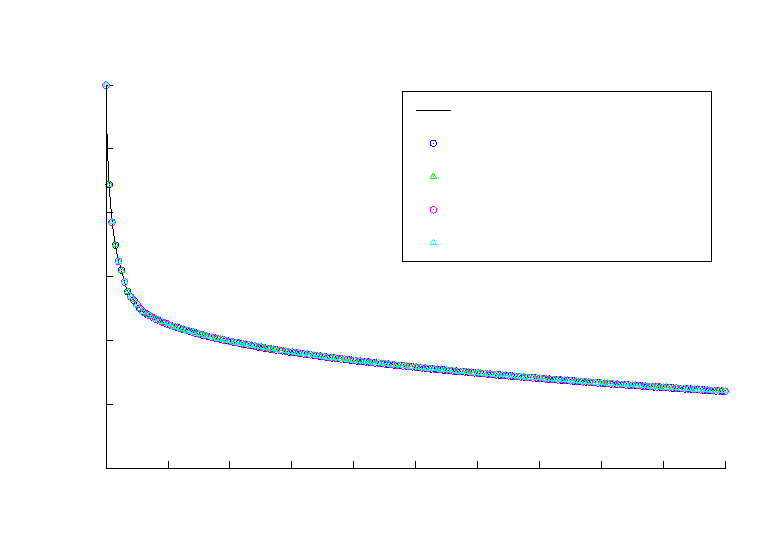
\includegraphics{xenon2_scale}}%
    \gplfronttext
  \end{picture}%
\endgroup
}
	\caption{•••}
	\label{fig:xenon2_scale}
\end{figure}
\begin{figure}
	\centering
	\resizebox{.9\textwidth}{!}{% GNUPLOT: LaTeX picture with Postscript
\begingroup
  \fontfamily{phv}%
  \selectfont
  \makeatletter
  \providecommand\color[2][]{%
    \GenericError{(gnuplot) \space\space\space\@spaces}{%
      Package color not loaded in conjunction with
      terminal option `colourtext'%
    }{See the gnuplot documentation for explanation.%
    }{Either use 'blacktext' in gnuplot or load the package
      color.sty in LaTeX.}%
    \renewcommand\color[2][]{}%
  }%
  \providecommand\includegraphics[2][]{%
    \GenericError{(gnuplot) \space\space\space\@spaces}{%
      Package graphicx or graphics not loaded%
    }{See the gnuplot documentation for explanation.%
    }{The gnuplot epslatex terminal needs graphicx.sty or graphics.sty.}%
    \renewcommand\includegraphics[2][]{}%
  }%
  \providecommand\rotatebox[2]{#2}%
  \@ifundefined{ifGPcolor}{%
    \newif\ifGPcolor
    \GPcolorfalse
  }{}%
  \@ifundefined{ifGPblacktext}{%
    \newif\ifGPblacktext
    \GPblacktexttrue
  }{}%
  % define a \g@addto@macro without @ in the name:
  \let\gplgaddtomacro\g@addto@macro
  % define empty templates for all commands taking text:
  \gdef\gplbacktext{}%
  \gdef\gplfronttext{}%
  \makeatother
  \ifGPblacktext
    % no textcolor at all
    \def\colorrgb#1{}%
    \def\colorgray#1{}%
  \else
    % gray or color?
    \ifGPcolor
      \def\colorrgb#1{\color[rgb]{#1}}%
      \def\colorgray#1{\color[gray]{#1}}%
      \expandafter\def\csname LTw\endcsname{\color{white}}%
      \expandafter\def\csname LTb\endcsname{\color{black}}%
      \expandafter\def\csname LTa\endcsname{\color{black}}%
      \expandafter\def\csname LT0\endcsname{\color[rgb]{1,0,0}}%
      \expandafter\def\csname LT1\endcsname{\color[rgb]{0,1,0}}%
      \expandafter\def\csname LT2\endcsname{\color[rgb]{0,0,1}}%
      \expandafter\def\csname LT3\endcsname{\color[rgb]{1,0,1}}%
      \expandafter\def\csname LT4\endcsname{\color[rgb]{0,1,1}}%
      \expandafter\def\csname LT5\endcsname{\color[rgb]{1,1,0}}%
      \expandafter\def\csname LT6\endcsname{\color[rgb]{0,0,0}}%
      \expandafter\def\csname LT7\endcsname{\color[rgb]{1,0.3,0}}%
      \expandafter\def\csname LT8\endcsname{\color[rgb]{0.5,0.5,0.5}}%
    \else
      % gray
      \def\colorrgb#1{\color{black}}%
      \def\colorgray#1{\color[gray]{#1}}%
      \expandafter\def\csname LTw\endcsname{\color{white}}%
      \expandafter\def\csname LTb\endcsname{\color{black}}%
      \expandafter\def\csname LTa\endcsname{\color{black}}%
      \expandafter\def\csname LT0\endcsname{\color{black}}%
      \expandafter\def\csname LT1\endcsname{\color{black}}%
      \expandafter\def\csname LT2\endcsname{\color{black}}%
      \expandafter\def\csname LT3\endcsname{\color{black}}%
      \expandafter\def\csname LT4\endcsname{\color{black}}%
      \expandafter\def\csname LT5\endcsname{\color{black}}%
      \expandafter\def\csname LT6\endcsname{\color{black}}%
      \expandafter\def\csname LT7\endcsname{\color{black}}%
      \expandafter\def\csname LT8\endcsname{\color{black}}%
    \fi
  \fi
    \setlength{\unitlength}{0.0500bp}%
    \ifx\gptboxheight\undefined%
      \newlength{\gptboxheight}%
      \newlength{\gptboxwidth}%
      \newsavebox{\gptboxtext}%
    \fi%
    \setlength{\fboxrule}{0.5pt}%
    \setlength{\fboxsep}{1pt}%
\begin{picture}(7200.00,5040.00)%
    \gplgaddtomacro\gplbacktext{%
      \csname LTb\endcsname%
      \put(726,704){\makebox(0,0)[r]{\strut{}\footnotesize -6}}%
      \put(726,1316){\makebox(0,0)[r]{\strut{}\footnotesize -5}}%
      \put(726,1929){\makebox(0,0)[r]{\strut{}\footnotesize -4}}%
      \put(726,2542){\makebox(0,0)[r]{\strut{}\footnotesize -3}}%
      \put(726,3154){\makebox(0,0)[r]{\strut{}\footnotesize -2}}%
      \put(726,3767){\makebox(0,0)[r]{\strut{}\footnotesize -1}}%
      \put(726,4379){\makebox(0,0)[r]{\strut{}\footnotesize 0}}%
      \put(1453,484){\makebox(0,0){\strut{}\footnotesize 100}}%
      \put(2047,484){\makebox(0,0){\strut{}\footnotesize 200}}%
      \put(2642,484){\makebox(0,0){\strut{}\footnotesize 300}}%
      \put(3236,484){\makebox(0,0){\strut{}\footnotesize 400}}%
      \put(3831,484){\makebox(0,0){\strut{}\footnotesize 500}}%
      \put(4425,484){\makebox(0,0){\strut{}\footnotesize 600}}%
      \put(5020,484){\makebox(0,0){\strut{}\footnotesize 700}}%
      \put(5614,484){\makebox(0,0){\strut{}\footnotesize 800}}%
      \put(6209,484){\makebox(0,0){\strut{}\footnotesize 900}}%
      \put(6803,484){\makebox(0,0){\strut{}\footnotesize 1000}}%
    }%
    \gplgaddtomacro\gplfronttext{%
      \csname LTb\endcsname%
      \put(352,2541){\rotatebox{-270}{\makebox(0,0){\strut{}\footnotesize Residual 2-norm, log scale}}}%
      \put(3830,154){\makebox(0,0){\strut{}\footnotesize Iteration count}}%
      \put(3830,4709){\makebox(0,0){\strut{}\shortstack{bcsstk18}}}%
      \csname LTb\endcsname%
      \put(4176,4175){\makebox(0,0)[l]{\strut{}\scriptsize GMRES(60)}}%
      \csname LTb\endcsname%
      \put(4176,3856){\makebox(0,0)[l]{\strut{}\begin{minipage}[l]{.95\textwidth} \scriptsize Monomial-GMRES(5,12) \newline \tiny min, max basis rcond \#: 2.02e-44, 2.90e-43\end{minipage}}}%
      \csname LTb\endcsname%
      \put(4176,3537){\makebox(0,0)[l]{\strut{}\begin{minipage}[l]{.95\textwidth} \scriptsize Newton-GMRES(5,12) \newline \tiny min, max basis rcond \#: 1.25e-42, 2.67e-40\end{minipage}}}%
      \csname LTb\endcsname%
      \put(4176,3218){\makebox(0,0)[l]{\strut{}\begin{minipage}[l]{.95\textwidth} \scriptsize Monomial-GMRES(10,6) \newline \tiny min, max basis rcond \#: 8.42e-98, 6.63e-96\end{minipage}}}%
      \csname LTb\endcsname%
      \put(4176,2899){\makebox(0,0)[l]{\strut{}\begin{minipage}[l]{.95\textwidth} \scriptsize Newton-GMRES(10,6) \newline \tiny min, max basis rcond \#: 4.06e-94, 8.41e-90\end{minipage}}}%
    }%
    \gplbacktext
    \put(0,0){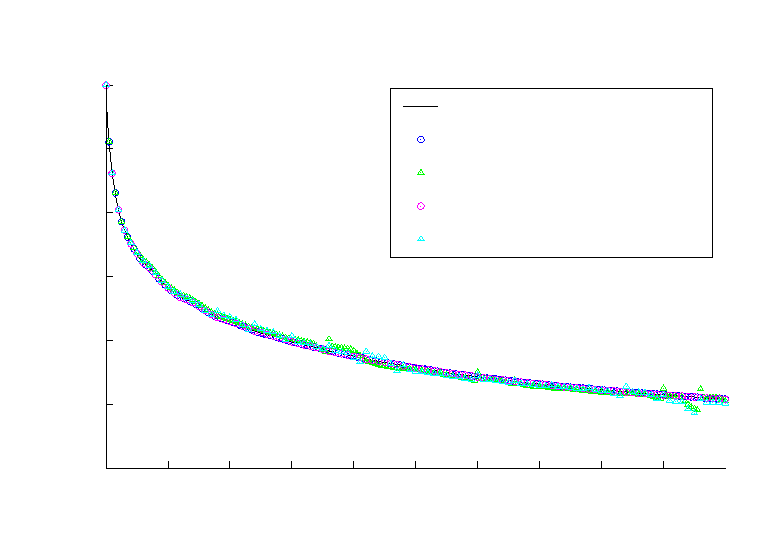
\includegraphics{bcsstk18_noscale}}%
    \gplfronttext
  \end{picture}%
\endgroup
}
	\caption{•••}
	\label{fig:bcsstk18_noscale}
\end{figure}
\begin{figure}
	\centering
	\resizebox{.9\textwidth}{!}{% GNUPLOT: LaTeX picture with Postscript
\begingroup
  \fontfamily{phv}%
  \selectfont
  \makeatletter
  \providecommand\color[2][]{%
    \GenericError{(gnuplot) \space\space\space\@spaces}{%
      Package color not loaded in conjunction with
      terminal option `colourtext'%
    }{See the gnuplot documentation for explanation.%
    }{Either use 'blacktext' in gnuplot or load the package
      color.sty in LaTeX.}%
    \renewcommand\color[2][]{}%
  }%
  \providecommand\includegraphics[2][]{%
    \GenericError{(gnuplot) \space\space\space\@spaces}{%
      Package graphicx or graphics not loaded%
    }{See the gnuplot documentation for explanation.%
    }{The gnuplot epslatex terminal needs graphicx.sty or graphics.sty.}%
    \renewcommand\includegraphics[2][]{}%
  }%
  \providecommand\rotatebox[2]{#2}%
  \@ifundefined{ifGPcolor}{%
    \newif\ifGPcolor
    \GPcolorfalse
  }{}%
  \@ifundefined{ifGPblacktext}{%
    \newif\ifGPblacktext
    \GPblacktexttrue
  }{}%
  % define a \g@addto@macro without @ in the name:
  \let\gplgaddtomacro\g@addto@macro
  % define empty templates for all commands taking text:
  \gdef\gplbacktext{}%
  \gdef\gplfronttext{}%
  \makeatother
  \ifGPblacktext
    % no textcolor at all
    \def\colorrgb#1{}%
    \def\colorgray#1{}%
  \else
    % gray or color?
    \ifGPcolor
      \def\colorrgb#1{\color[rgb]{#1}}%
      \def\colorgray#1{\color[gray]{#1}}%
      \expandafter\def\csname LTw\endcsname{\color{white}}%
      \expandafter\def\csname LTb\endcsname{\color{black}}%
      \expandafter\def\csname LTa\endcsname{\color{black}}%
      \expandafter\def\csname LT0\endcsname{\color[rgb]{1,0,0}}%
      \expandafter\def\csname LT1\endcsname{\color[rgb]{0,1,0}}%
      \expandafter\def\csname LT2\endcsname{\color[rgb]{0,0,1}}%
      \expandafter\def\csname LT3\endcsname{\color[rgb]{1,0,1}}%
      \expandafter\def\csname LT4\endcsname{\color[rgb]{0,1,1}}%
      \expandafter\def\csname LT5\endcsname{\color[rgb]{1,1,0}}%
      \expandafter\def\csname LT6\endcsname{\color[rgb]{0,0,0}}%
      \expandafter\def\csname LT7\endcsname{\color[rgb]{1,0.3,0}}%
      \expandafter\def\csname LT8\endcsname{\color[rgb]{0.5,0.5,0.5}}%
    \else
      % gray
      \def\colorrgb#1{\color{black}}%
      \def\colorgray#1{\color[gray]{#1}}%
      \expandafter\def\csname LTw\endcsname{\color{white}}%
      \expandafter\def\csname LTb\endcsname{\color{black}}%
      \expandafter\def\csname LTa\endcsname{\color{black}}%
      \expandafter\def\csname LT0\endcsname{\color{black}}%
      \expandafter\def\csname LT1\endcsname{\color{black}}%
      \expandafter\def\csname LT2\endcsname{\color{black}}%
      \expandafter\def\csname LT3\endcsname{\color{black}}%
      \expandafter\def\csname LT4\endcsname{\color{black}}%
      \expandafter\def\csname LT5\endcsname{\color{black}}%
      \expandafter\def\csname LT6\endcsname{\color{black}}%
      \expandafter\def\csname LT7\endcsname{\color{black}}%
      \expandafter\def\csname LT8\endcsname{\color{black}}%
    \fi
  \fi
    \setlength{\unitlength}{0.0500bp}%
    \ifx\gptboxheight\undefined%
      \newlength{\gptboxheight}%
      \newlength{\gptboxwidth}%
      \newsavebox{\gptboxtext}%
    \fi%
    \setlength{\fboxrule}{0.5pt}%
    \setlength{\fboxsep}{1pt}%
\begin{picture}(7200.00,5040.00)%
    \gplgaddtomacro\gplbacktext{%
      \csname LTb\endcsname%
      \put(726,704){\makebox(0,0)[r]{\strut{}\footnotesize -6}}%
      \put(726,1316){\makebox(0,0)[r]{\strut{}\footnotesize -5}}%
      \put(726,1929){\makebox(0,0)[r]{\strut{}\footnotesize -4}}%
      \put(726,2542){\makebox(0,0)[r]{\strut{}\footnotesize -3}}%
      \put(726,3154){\makebox(0,0)[r]{\strut{}\footnotesize -2}}%
      \put(726,3767){\makebox(0,0)[r]{\strut{}\footnotesize -1}}%
      \put(726,4379){\makebox(0,0)[r]{\strut{}\footnotesize 0}}%
      \put(1453,484){\makebox(0,0){\strut{}\footnotesize 100}}%
      \put(2047,484){\makebox(0,0){\strut{}\footnotesize 200}}%
      \put(2642,484){\makebox(0,0){\strut{}\footnotesize 300}}%
      \put(3236,484){\makebox(0,0){\strut{}\footnotesize 400}}%
      \put(3831,484){\makebox(0,0){\strut{}\footnotesize 500}}%
      \put(4425,484){\makebox(0,0){\strut{}\footnotesize 600}}%
      \put(5020,484){\makebox(0,0){\strut{}\footnotesize 700}}%
      \put(5614,484){\makebox(0,0){\strut{}\footnotesize 800}}%
      \put(6209,484){\makebox(0,0){\strut{}\footnotesize 900}}%
    }%
    \gplgaddtomacro\gplfronttext{%
      \csname LTb\endcsname%
      \put(352,2541){\rotatebox{-270}{\makebox(0,0){\strut{}\footnotesize Residual 2-norm, log scale}}}%
      \put(3830,154){\makebox(0,0){\strut{}\footnotesize Iteration count}}%
      \put(3830,4709){\makebox(0,0){\strut{}\shortstack{bcsstk18}}}%
      \csname LTb\endcsname%
      \put(4176,4175){\makebox(0,0)[l]{\strut{}\scriptsize GMRES(60)}}%
      \csname LTb\endcsname%
      \put(4176,3856){\makebox(0,0)[l]{\strut{}\begin{minipage}[l]{.95\textwidth} \scriptsize Monomial-GMRES(5,12) \newline \tiny min, max basis rcond \#: 1.67e-04, 1.09e-03\end{minipage}}}%
      \csname LTb\endcsname%
      \put(4176,3537){\makebox(0,0)[l]{\strut{}\begin{minipage}[l]{.95\textwidth} \scriptsize Newton-GMRES(5,12) \newline \tiny min, max basis rcond \#: 1.35e-03, 2.09e-01\end{minipage}}}%
      \csname LTb\endcsname%
      \put(4176,3218){\makebox(0,0)[l]{\strut{}\begin{minipage}[l]{.95\textwidth} \scriptsize Monomial-GMRES(10,6) \newline \tiny min, max basis rcond \#: 6.80e-09, 1.51e-07\end{minipage}}}%
      \csname LTb\endcsname%
      \put(4176,2899){\makebox(0,0)[l]{\strut{}\begin{minipage}[l]{.95\textwidth} \scriptsize Newton-GMRES(10,6) \newline \tiny min, max basis rcond \#: 3.06e-17, 9.12e-03\end{minipage}}}%
    }%
    \gplbacktext
    \put(0,0){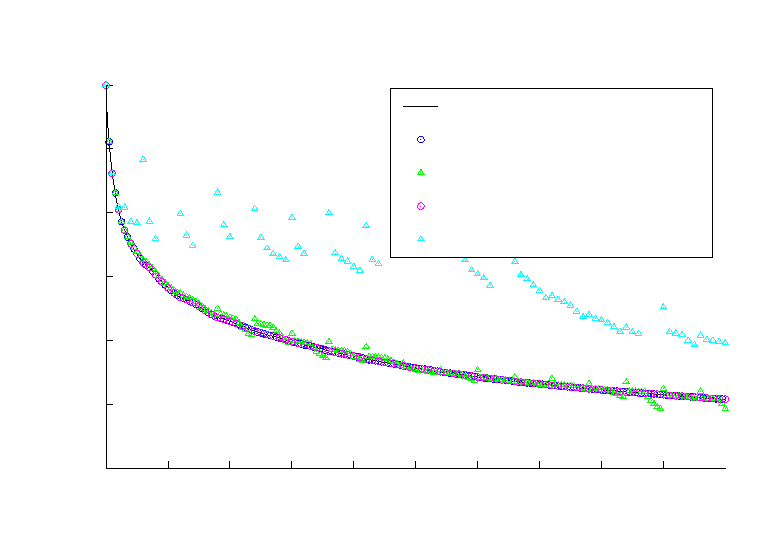
\includegraphics{bcsstk18_scale}}%
    \gplfronttext
  \end{picture}%
\endgroup
}
	\caption{•••}
	\label{fig:bcsstk18_scale}
\end{figure}

\section{Performance experiments}
\begin{figure}[H]
	\centering
	\resizebox{1.0\textwidth}{!}{% GNUPLOT: LaTeX picture with Postscript
\begingroup
  \fontfamily{phv}%
  \selectfont
  \makeatletter
  \providecommand\color[2][]{%
    \GenericError{(gnuplot) \space\space\space\@spaces}{%
      Package color not loaded in conjunction with
      terminal option `colourtext'%
    }{See the gnuplot documentation for explanation.%
    }{Either use 'blacktext' in gnuplot or load the package
      color.sty in LaTeX.}%
    \renewcommand\color[2][]{}%
  }%
  \providecommand\includegraphics[2][]{%
    \GenericError{(gnuplot) \space\space\space\@spaces}{%
      Package graphicx or graphics not loaded%
    }{See the gnuplot documentation for explanation.%
    }{The gnuplot epslatex terminal needs graphicx.sty or graphics.sty.}%
    \renewcommand\includegraphics[2][]{}%
  }%
  \providecommand\rotatebox[2]{#2}%
  \@ifundefined{ifGPcolor}{%
    \newif\ifGPcolor
    \GPcolorfalse
  }{}%
  \@ifundefined{ifGPblacktext}{%
    \newif\ifGPblacktext
    \GPblacktexttrue
  }{}%
  % define a \g@addto@macro without @ in the name:
  \let\gplgaddtomacro\g@addto@macro
  % define empty templates for all commands taking text:
  \gdef\gplbacktext{}%
  \gdef\gplfronttext{}%
  \makeatother
  \ifGPblacktext
    % no textcolor at all
    \def\colorrgb#1{}%
    \def\colorgray#1{}%
  \else
    % gray or color?
    \ifGPcolor
      \def\colorrgb#1{\color[rgb]{#1}}%
      \def\colorgray#1{\color[gray]{#1}}%
      \expandafter\def\csname LTw\endcsname{\color{white}}%
      \expandafter\def\csname LTb\endcsname{\color{black}}%
      \expandafter\def\csname LTa\endcsname{\color{black}}%
      \expandafter\def\csname LT0\endcsname{\color[rgb]{1,0,0}}%
      \expandafter\def\csname LT1\endcsname{\color[rgb]{0,1,0}}%
      \expandafter\def\csname LT2\endcsname{\color[rgb]{0,0,1}}%
      \expandafter\def\csname LT3\endcsname{\color[rgb]{1,0,1}}%
      \expandafter\def\csname LT4\endcsname{\color[rgb]{0,1,1}}%
      \expandafter\def\csname LT5\endcsname{\color[rgb]{1,1,0}}%
      \expandafter\def\csname LT6\endcsname{\color[rgb]{0,0,0}}%
      \expandafter\def\csname LT7\endcsname{\color[rgb]{1,0.3,0}}%
      \expandafter\def\csname LT8\endcsname{\color[rgb]{0.5,0.5,0.5}}%
    \else
      % gray
      \def\colorrgb#1{\color{black}}%
      \def\colorgray#1{\color[gray]{#1}}%
      \expandafter\def\csname LTw\endcsname{\color{white}}%
      \expandafter\def\csname LTb\endcsname{\color{black}}%
      \expandafter\def\csname LTa\endcsname{\color{black}}%
      \expandafter\def\csname LT0\endcsname{\color{black}}%
      \expandafter\def\csname LT1\endcsname{\color{black}}%
      \expandafter\def\csname LT2\endcsname{\color{black}}%
      \expandafter\def\csname LT3\endcsname{\color{black}}%
      \expandafter\def\csname LT4\endcsname{\color{black}}%
      \expandafter\def\csname LT5\endcsname{\color{black}}%
      \expandafter\def\csname LT6\endcsname{\color{black}}%
      \expandafter\def\csname LT7\endcsname{\color{black}}%
      \expandafter\def\csname LT8\endcsname{\color{black}}%
    \fi
  \fi
    \setlength{\unitlength}{0.0500bp}%
    \ifx\gptboxheight\undefined%
      \newlength{\gptboxheight}%
      \newlength{\gptboxwidth}%
      \newsavebox{\gptboxtext}%
    \fi%
    \setlength{\fboxrule}{0.5pt}%
    \setlength{\fboxsep}{1pt}%
\begin{picture}(7200.00,5040.00)%
    \gplgaddtomacro\gplbacktext{%
      \csname LTb\endcsname%
      \put(688,512){\makebox(0,0)[r]{\strut{}\footnotesize 0}}%
      \csname LTb\endcsname%
      \put(688,994){\makebox(0,0)[r]{\strut{}\footnotesize 0.5}}%
      \csname LTb\endcsname%
      \put(688,1476){\makebox(0,0)[r]{\strut{}\footnotesize 1}}%
      \csname LTb\endcsname%
      \put(688,1957){\makebox(0,0)[r]{\strut{}\footnotesize 1.5}}%
      \csname LTb\endcsname%
      \put(688,2439){\makebox(0,0)[r]{\strut{}\footnotesize 2}}%
      \csname LTb\endcsname%
      \put(688,2921){\makebox(0,0)[r]{\strut{}\footnotesize 2.5}}%
      \csname LTb\endcsname%
      \put(688,3403){\makebox(0,0)[r]{\strut{}\footnotesize 3}}%
      \csname LTb\endcsname%
      \put(688,3885){\makebox(0,0)[r]{\strut{}\footnotesize 3.5}}%
      \csname LTb\endcsname%
      \put(688,4366){\makebox(0,0)[r]{\strut{}\footnotesize 4}}%
      \csname LTb\endcsname%
      \put(1350,352){\makebox(0,0){\strut{}\footnotesize\,watt1}}%
      \csname LTb\endcsname%
      \put(2619,352){\makebox(0,0){\strut{}\footnotesize\,sherman3}}%
      \csname LTb\endcsname%
      \put(3889,352){\makebox(0,0){\strut{}\footnotesize\,bcsstk18}}%
      \csname LTb\endcsname%
      \put(5159,352){\makebox(0,0){\strut{}\footnotesize\,xenon2}}%
      \csname LTb\endcsname%
      \put(6429,352){\makebox(0,0){\strut{}\footnotesize\,pwtk}}%
    }%
    \gplgaddtomacro\gplfronttext{%
      \csname LTb\endcsname%
      \put(128,2535){\rotatebox{-270}{\makebox(0,0){\strut{}\footnotesize Runtime / runtime(CA-GMRES)}}}%
      \put(3895,112){\makebox(0,0){\strut{}\footnotesize Sparse matrix}}%
      \put(3895,4799){\makebox(0,0){\strut{}\shortstack{\footnotesize\,Runtime\,per\,kernel,\,relative\,to\,CA-GMRES\,with\,best\,s\,and\,restart\,length\\\footnotesize\,for\,all\,test\,matrices\,using\,8\,threads.}}}%
      \csname LTb\endcsname%
      \put(1129,1600){\makebox(0,0){\strut{}1.3x}}%
      \put(2399,1600){\makebox(0,0){\strut{}2.1x}}%
      \put(3669,1600){\makebox(0,0){\strut{}4.0x}}%
      \put(4938,1600){\makebox(0,0){\strut{}2.4x}}%
      \put(6208,1600){\makebox(0,0){\strut{}2.2x}}%
      \csname LTb\endcsname%
      \put(1519,3600){\makebox(0,0)[l]{\strut{}\scriptsize Small dense operations}}%
      \csname LTb\endcsname%
      \put(1519,3760){\makebox(0,0)[l]{\strut{}\scriptsize Block Gram-Schmidt}}%
      \csname LTb\endcsname%
      \put(1519,3920){\makebox(0,0)[l]{\strut{}\scriptsize TSQR}}%
      \csname LTb\endcsname%
      \put(1519,4080){\makebox(0,0)[l]{\strut{}\scriptsize SpMV}}%
      \csname LTb\endcsname%
      \put(1519,4240){\makebox(0,0)[l]{\strut{}\scriptsize INIT}}%
      \csname LTb\endcsname%
      \put(1519,4400){\makebox(0,0)[l]{\strut{}\scriptsize MGS}}%
    }%
    \gplbacktext
    \put(0,0){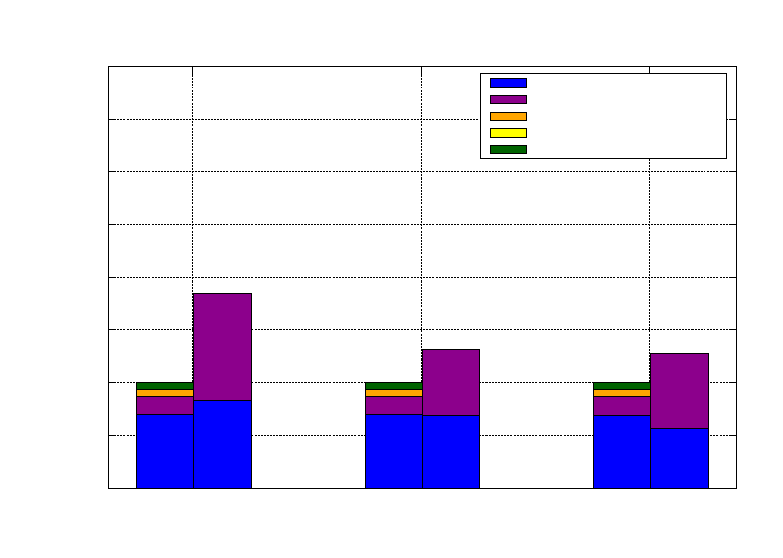
\includegraphics{runtimes_matrices}}%
    \gplfronttext
  \end{picture}%
\endgroup
}
	\caption{left CA-GMRES, right GMRES}
\end{figure}

\section{Conclusion}
Conclusion: the MPK is an important kernel and should have been implemented, also restarting with $s$ steps of std. GMRES is not optimal and leaves room for optimization.
\iffalse
compute Ritz values of real upper Hessenberg matrix with LAPACK "DHSEQR()"
\url{http://www.netlib.org/lapack/explore-html/da/dba/group__double_o_t_h_e_rcomputational_gacb35e85b362ce8ccf9d653cc3f8fb89c.html#gacb35e85b362ce8ccf9d653cc3f8fb89c}
\\

Modified Leja ordering \cite{Hoemmen:2010:CKS:1970638} p.291/292\\

Octave code:\\
\url{https://github.com/magnusgrandin/ca-lanczos/blob/master/modified_leja.m}
\fi

\iffalse
\section*{Krylov subspace methods (summarize this section briefly in introduction)}

\cite{Ascher:2011:FCN:2031413} p.191\\
\begin{itemize}
\item short description:\\
Krylov subspace definition: $\mathcal{K}_k(A, r_0) = span \left\{ r_0, Ar_0, A^2r_0,\ldots,A^{k-1}r_0 \right\}$\\

All iterative methods build and enhance a KSP with every iteration.
\begin{equation*}
\textbf{r}_k = \textbf{r}_0 + \sum_{j=1}^{k} c_jA^j\textbf{r}_0 \quad \to \quad \textbf{x}_k = \textbf{x}_0 + \sum_{j=0}^{k-1} c_{j+1}A^j\textbf{r}_0
\end{equation*}
what is good for the power method, is bad here, bc. vectors are in theory linearly independent but too close to parallel $\to$ in machine arithmetic they become linearly dependent. Need new basis \ldots 
\item Arnoldi \cite{Ascher:2011:FCN:2031413} p.192
\begin{equation*}
AQ_k = Q_{k+1}H_{k+1,k}
\end{equation*}
\item Summary: (\cite{Ascher:2011:FCN:2031413} p. 192)
	\begin{itemize}
	\item 1. construct an orthogonal basis for the Krylov subspace;
	\item 2. define an optimality property;
	\item 3. use an effective preconditioner.
	\end{itemize}
\end{itemize}

\cite{Ascher:2011:FCN:2031413} p.184\\
\begin{itemize}
\item short description: most stable and prominent iterative method, for sym pos def matrices only.
\item Algorithm description (just the basics)
	\begin{itemize}
	\item $\norm{x - x_k}_A = \text{argmin}_{y \in \mathcal{K}_k(A, r_0)}\norm{x - y}_A$\\
	 After $k$-steps, $x_k$ minimizes in the KSP the $A$-norm x - $y$ (only if A is SPD, or else it's not a norm)
	\item follows basic concept: $\textbf{x}_{new} = x_{old} + constant \cdot search direction$ (better version \textit{steepest descent})
	\item $\textbf{r}_k$ is multiple of $q_{k+1}$ ($q$ from Arnoldi; $q$ is not directly used in CG)\\
	$\to$ (1) orthogonal residuals $\textbf{r}_i^T\textbf{r}_k = 0, \quad i < k$\\
	$\to$ (2) $(x_i - x_{i-1})^T A (x_k - x_{k-1}) = 0 \quad \to \quad\Delta \textbf{x}_i^T A \Delta \textbf{x}_k = 0, \quad  i < k$\\
	in other words: the corrections in \textbf{x} are orthogonal in the $A$-inner product, hence the term 'conjugate' in CG. The term 'gradients' comes from minimizing the energy equation/quadratic form:
	\begin{equation*}
	E(x) = \frac{1}{2} \textbf{x}^TA\textbf{x} - b^T\textbf{x} \to min
	\end{equation*}	 
	Set the derivative (gradient) to zero, i.e. $E'(x) = 0$:
	\begin{equation*}
	A\textbf{x} - b = 0
	\end{equation*}
	and we're back to the original problem. So minimizing energies and solving the linear equation $A\textbf{x} = b$ are basically the same.
	\item $H$ is symmetric, and therefore tridiagonal. Arnoldi simplifies to Lanczos $\to$ short 'three-term' recurrences (only have to look at a few previous orthogonal vectors, not all of them).
	\end{itemize}
\item p.191 what about general matrices? Any nonsingular matrix $A$ can be transformed into SPD matrix via $A^TA$ $\to$ bad condition number $\kappa (A)$.\\

\{The condition number of the matrix $A^TA$ is the square of the condition number of $A$ [\ldots] A large condition number both increases the number of iterations required and limits the accuracy to which a solution can be obtained. \cite{press92a} p. 89 (2.7.40)\}
consider Krylov subspace methods that are directly based on general matrix $A$ $\to$ GMRES
\end{itemize}

\subsection*{GMRES (summarize this section briefly in introduction)}
\begin{itemize}
\item short description: general form of MINRES (=like CG it is only for symmetric matrices, but must not be PD) MINRES minimizes $\norm{\textbf{r}_k}_2$ and CG minimizes energy norm of the residual $\norm{\textbf{r}_k}_{A^{-1}}$ or the energy norm of the error $\norm{\textbf{x}^* - \textbf{x}_k}_A$ respectively. \cite{Ascher:2011:FCN:2031413} (p. 198)
\item algorithm description:
\item $\norm{b - A\textbf{x}_k}_2 = argmin_{y \in \mathcal{K}_k(A, r_0)}\norm{b - Ay}_2$\\
	 After $k$-steps, $\textbf{x}_k$ minimizes in the KSP the $\ell^2$-norm $b - Ay$
\item GMRES vs. CG:
\begin{itemize}
\item CG forces the residual $\textbf{r}_k$ to be orthogonal to the Krylov subspace $\mathcal{K}_k(A, r_0)$;
\item GMRES seeks the residual with minimum $\ell_2$-norm within the Krylov subspace.
\end{itemize}
\item Summary:\\
The main components of a single iteration of GMRES are
\begin{enumerate}
	\item perform a step of the Arnoldi process;
	\item update the QR factorization of the updated upper Hessenberg matrix;
	\item solve the resulting least squares problem.
	\end{enumerate}
\end{itemize}
\fi
\bibliographystyle{plain}
\bibliography{BSc_Ernstbrunner_01403753}
 \listofalgorithms
\begin{appendices}
\section{Test matrices}
discussion of test matrices \\

\begin{tabular}{l|r|r}
Name & Dim & nnz \\
\hline
bmw & 141K & 3.7M \\
bcsstk18 & 12K & 149K \\
pwtk & 218K & 3.7M \\
watt1 & 1856 & 11550 \\
xenon2 & 157K & 3.9M
\end{tabular}

\section{TODO}
\begin{itemize}
\item describe CA-GMRES
\item write implementation details
\item write numerical experiments
\item write performance experiments
\item write introduction
\item write abstract
\end{itemize}
\end{appendices}
\end{document}
% End of document.